\chapter{第三方工具}
\label{chap:Third-Party Tools}

為了支援 HIP/ROCm 開發,目前已有許多第三方工具。本章簡要介紹了其中一些工具,並提供了在何處可以找到更多資訊的指示。

\section{\term{PAPI}}
\subsection{Introduction}

高效能運算(High Performance Computing, HPC)應用程式的開發過程往往需要耗費大量時間且複雜。許多程式需要高效地利用底層的硬體和軟體堆疊。透過詳細的測量,使用廣泛的效能計數器來量化不同硬體資源的使用效率。過去二十多年來,HPC 社群一直依賴 PAPI 監控庫來追蹤低階硬體操作。除了追蹤傳統的 CPU 計數器(如執行的指令數量,以及浮點運算、已完成指令、快取訪問和失敗等事件),PAPI 的最新發展也支持對 GPU(如 AMD、Intel 和 NVIDIA)的計數器進行監控,包括通訊網路、輸入/輸出(I/O)系統、能源監控及功率限制元件。PAPI 能夠通過單一的圖形使用者介面(GUI)收集整個計算系統的效能計數器數據。

除了硬體層面的計數器,PAPI 還提供了來自軟體層的計數器(軟體定義事件,SDEs)。這些計數器允許程式開發者從其函式庫中匯出任意資訊。例如,一個任務排程執行時可能會利用 SDEs 匯出內部的效能相關資訊,如「不同比例時間點的可用任務數量」等數據項目。


\begin{figure}
    \centering
    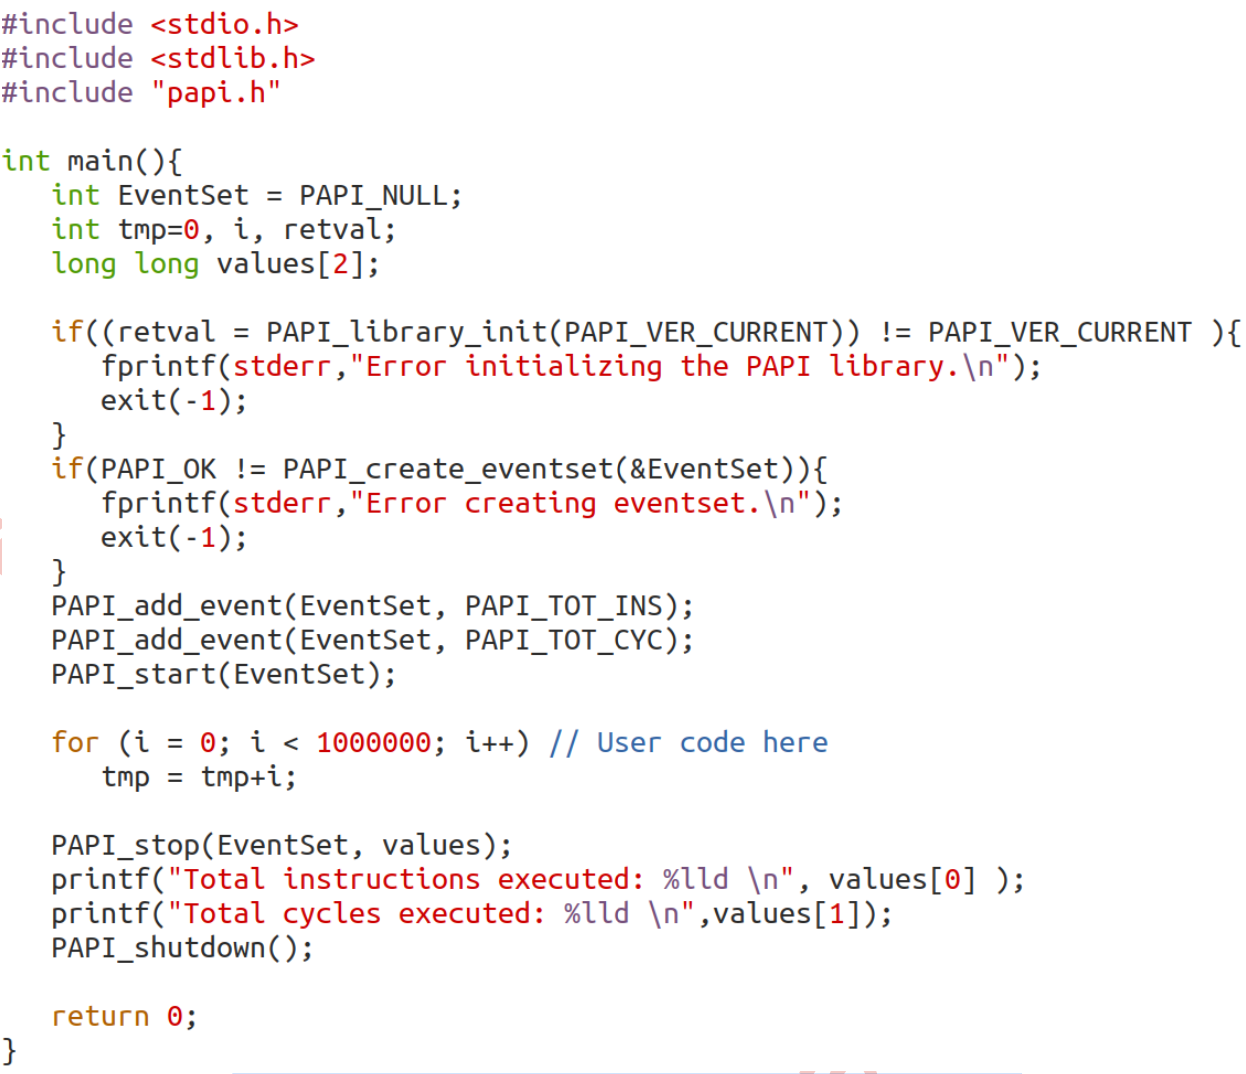
\includegraphics[width=0.9\linewidth]{FileAusiliari/Screenshots/Figure13-1.png}
    \caption{在程式中使用 PAPI 的範例。}
    \label{fig:PAPI}
\end{figure}

PAPI 透過相同的 PAPI\_start()、PAPI\_stop() 和 PAPI\_read() 的 GUI 指令,能夠監控硬體與軟體事件,從而更有效率地調整異質性硬體資源,並呈現應用程式完整的效能概況。除了直接使用 PAPI 之外,程式開發者也可以利用整合 PAPI 作為效能計數器監控後端的效能框架。這些工具採用硬體計數器抽樣、呼叫路徑追蹤及二進位分析的方式,生成圖形化的效能剖析,能將計數器值與應用程式中特定程式碼行所花費的時間聯繫起來。整合效能框架的例子包括 Arm MAP、HPCToolkit 和 TAU。


\subsection{PAPI 實用程式和測試}

除了用於監控事件的 API,PAPI 還提供了一些命令列工具,如下所示:
\begin{itemize}
    \item \texttt{papi\_component\_avail}. 提供已配置元件的相關資訊(見圖 13.2)。
    \item \texttt{papi\_avail}. 顯示預設事件及其在特定機器上的可用性資訊(見圖 13.3)。
    \item \texttt{papi\_native\_avail}. 提供原生事件的相關資訊(見圖 13.4)。
    \item \texttt{papi\_command\_line}. 允許使用者透過命令列介面測試事件(見圖 13.5)。
\end{itemize}

\begin{figure}
    \centering
    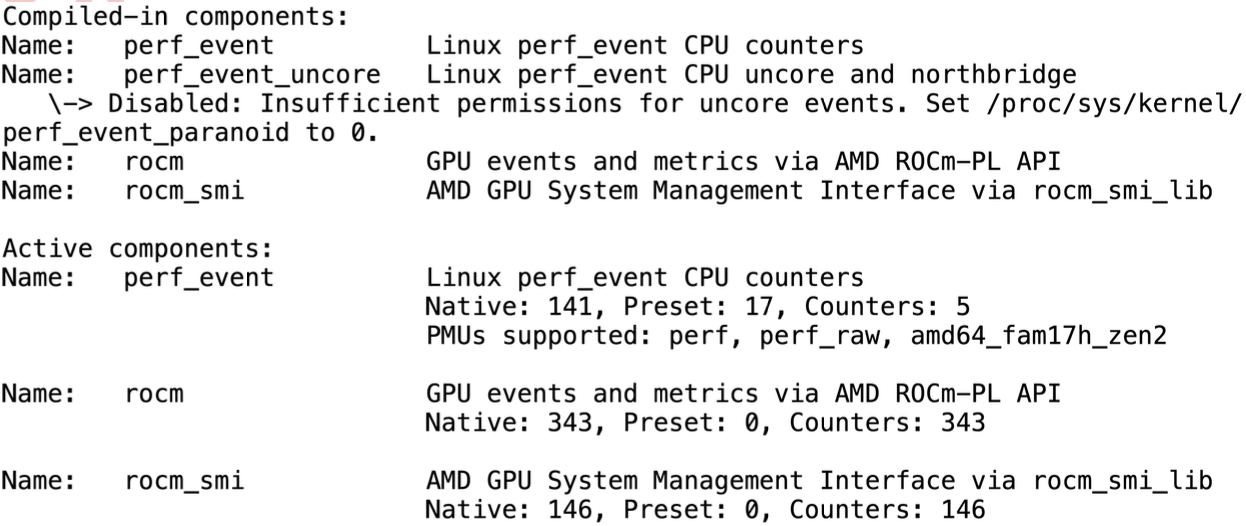
\includegraphics[width=0.9\linewidth]{FileAusiliari/Screenshots/Figure13-2.png}
    \caption{papi_component_avail.}
    \label{fig:PAPI2}
\end{figure}

\begin{figure}
    \centering
    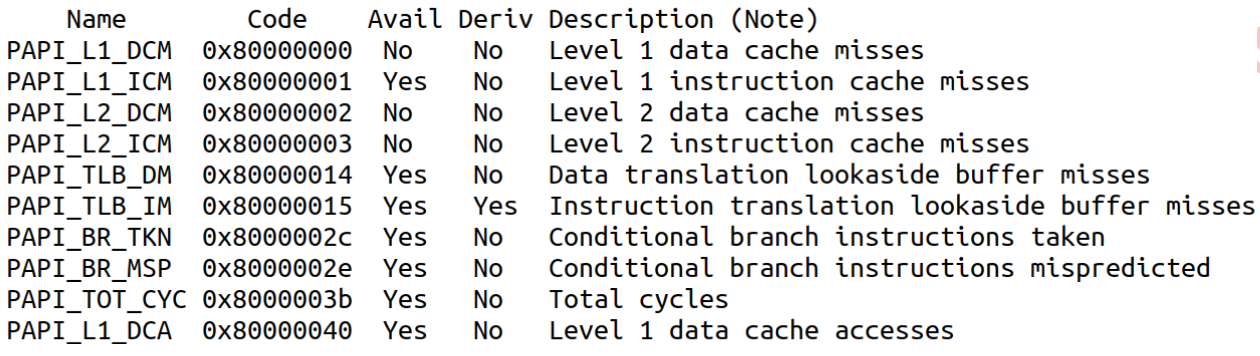
\includegraphics[width=0.9\linewidth]{FileAusiliari/Screenshots/Figure13-3.png}
    \caption{papi_avail.}
    \label{fig:PAPI3}
\end{figure}

\begin{figure}
    \centering
    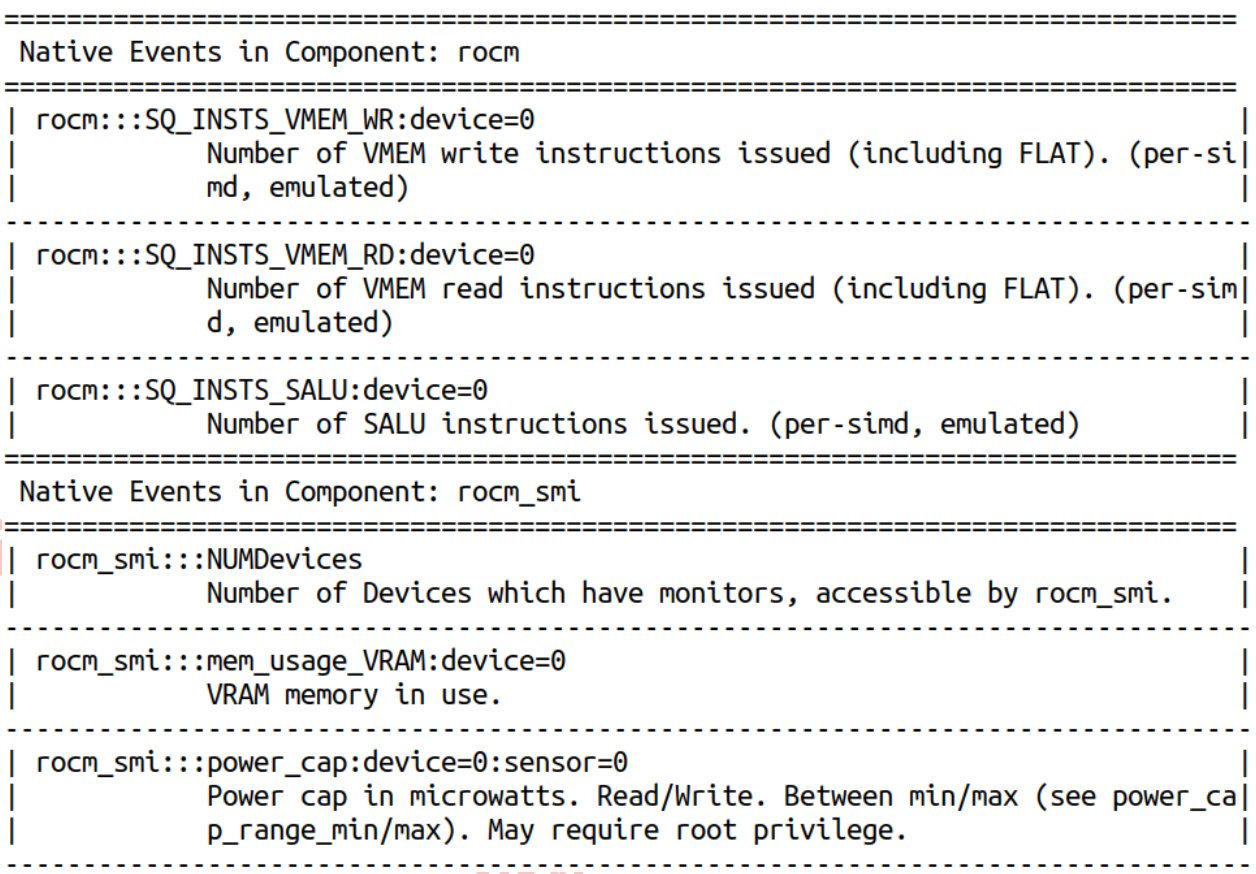
\includegraphics[width=0.9\linewidth]{FileAusiliari/Screenshots/Figure13-4.png}
    \caption{papi\_native\_avail.}
    \label{fig:PAPI4}
\end{figure}


\subsection{PAPI 對AMD GPU的支援}

PAPI 6.0.0 版本新增了對多個新元件的支援,包括 ROCm(支援 AMD GPU 上的效能計數器)和 rocm\_smi(監控功耗)。這些新增功能使程式開發者能夠更新電源設定並控制其效用。


\subsubsection{PAPI ROCm 元件}

PAPI ROCm 元件介接 AMD 的 ROCm 分析庫(即 rocProfiler),並支援監控 AMD GPU 上的硬體效能計數器。以下是部分監控功能的範例:

\begin{itemize}
    \item \texttt{LDS}:本地數據存儲(LDS)相關事件。
    \item \texttt{GDS}:全局數據存儲(GDS)相關事件。
    \item \texttt{TCP/TA}:L1 快取相關計數。
    \item \texttt{TCC}:L2 快取相關計數。
    \item \texttt{SQ}:指令調度器(Sequencer),包括指令的擷取、解碼與排程。
    \item \texttt{FLAT}:包括 Video、Sys、LDS 和 Scratch 的記憶體指令,使用flat address space,速度較慢。
    \item \texttt{VMEM}:向量記憶體儲存相關事件。
    \item \texttt{VMem}:影像記憶體相關事件。
    \item \texttt{SMEM}:純量記憶體儲存相關事件。
    \item \texttt{SFetch}:純量fetch事件。    
    \item \texttt{VFetch}:向量fetch事件(不包括 FLAT 指令)。
    \item \texttt{VALU}:向量運算單元(Vector ALU)相關事件。
    \item \texttt{SALU}:純量運算單元(Scalar ALU)相關事件(不包括浮點計數)。
\end{itemize}

\begin{figure}
    \centering
    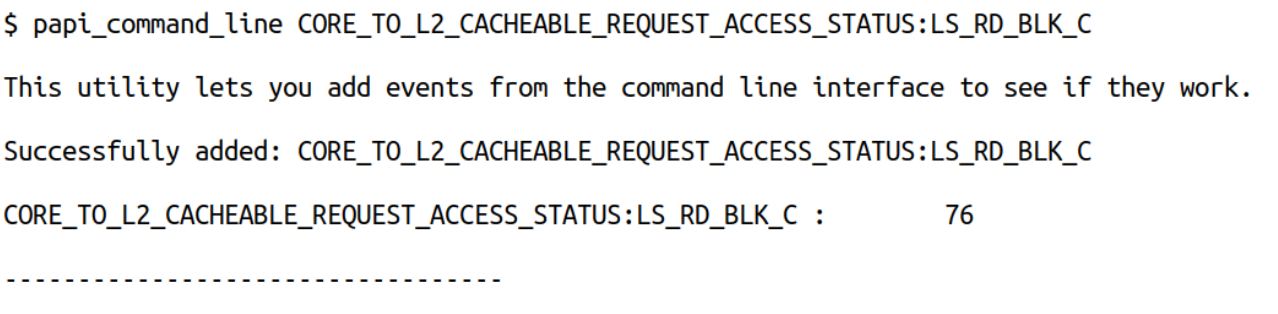
\includegraphics[width=0.9\linewidth]{FileAusiliari/Screenshots/Figure13-5.png}
    \caption{papi\_command\_line.}
    \label{fig:PAPI5}
\end{figure}

在圖 13.6 中,展示了在執行 rocBLAS GEMM kernel期間,使用 PAPI\_read() 每 5 毫秒收集的 AMD MI100 GPU L2 快取命中數據。

\subsubsection{PAPI rocm\_smi 元件}

PAPI rocm\_smi 元件與 AMD SMI 介接,新增了對電源管理的支援,使其能夠監控並限制 AMD GPU 的功率。這項新增功能讓科學應用程式開發者可以透過修改運行設定檔來降低能源成本。以下是該元件的監控功能範例:

\begin{itemize}
    \item \texttt{Power}:監控與限制功率。
    \item \texttt{Temperature}:包括目前溫度、最高臨界值以及臨時緊急溫度。
    \item \texttt{Fan}:以每分鐘轉速(RPM)顯示風扇速度、最大速度,以及讀寫速度。
    \item \texttt{Memory}:包括總 VRAM、可見 VRAM,以及圖形轉換表(GTT)VRAM。
    \item \texttt{PCI}:監控傳輸吞吐量、接收量以及最大封包大小。
    \item \texttt{Busy percent}:device忙於處理的時間百分比。
\end{itemize}

在圖 13.7 的例子中,展示了在運行 hipBLAS GEMM 核心期間,PAPI\_read() 收集的 AMD MI60 GPU 精細化功耗數據樣本。

\subsection{預設事件和計數器分析工具包 (CAT)}

\begin{figure}
    \centering
    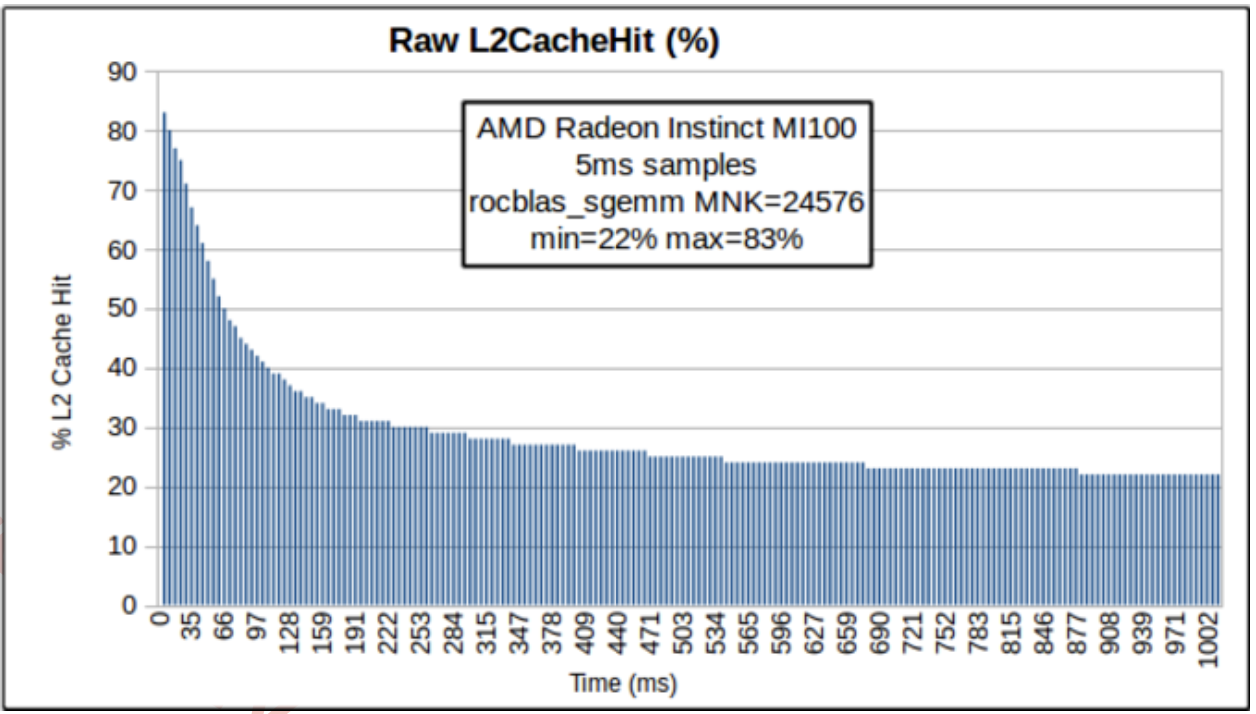
\includegraphics[width=0.9\linewidth]{FileAusiliari/Screenshots/Figure13-6.png}
    \caption{AMD MI100 GPU 上的 L2 快取 SGEMM 命中率。}
    \label{fig:PAPI6}
\end{figure}

PAPI 除了允許存取低階硬體計數器外,還提供了一組較高階的事件,這些事件在抽象微架構細節的同時,保持跨供應商與硬體世代一致的名稱。例如,PAPI\_L2\_DCR 就是一個預設事件。該事件計數器被配置為統計 L2 快取的讀取請求數。

預設事件的重要性有兩方面:
首先,使用可移植且直觀的事件名稱更為方便。
接著,它們設計為更容易映射到性能概念,便於理解和應用。
為了幫助程式設計師選擇原生事件或其組合來定義預設事件,PAPI 提供了一組範例供參考。此外,預設事件和計數器分析工具包(CAT) 也是 PAPI 的一部分,可用於輔助事件選擇與配置。



% \begin{verbatim}
% ./cat_collect -in event_list.txt -out OUT_DIR -dcr
% \end{verbatim}


\begin{lstlisting}
./cat_collect -in event_list.txt -out OUT_DIR -dcr
\end{lstlisting}

\section{Score-P 和 Vampir}

\subsection{概述}

\begin{figure}
    \centering
    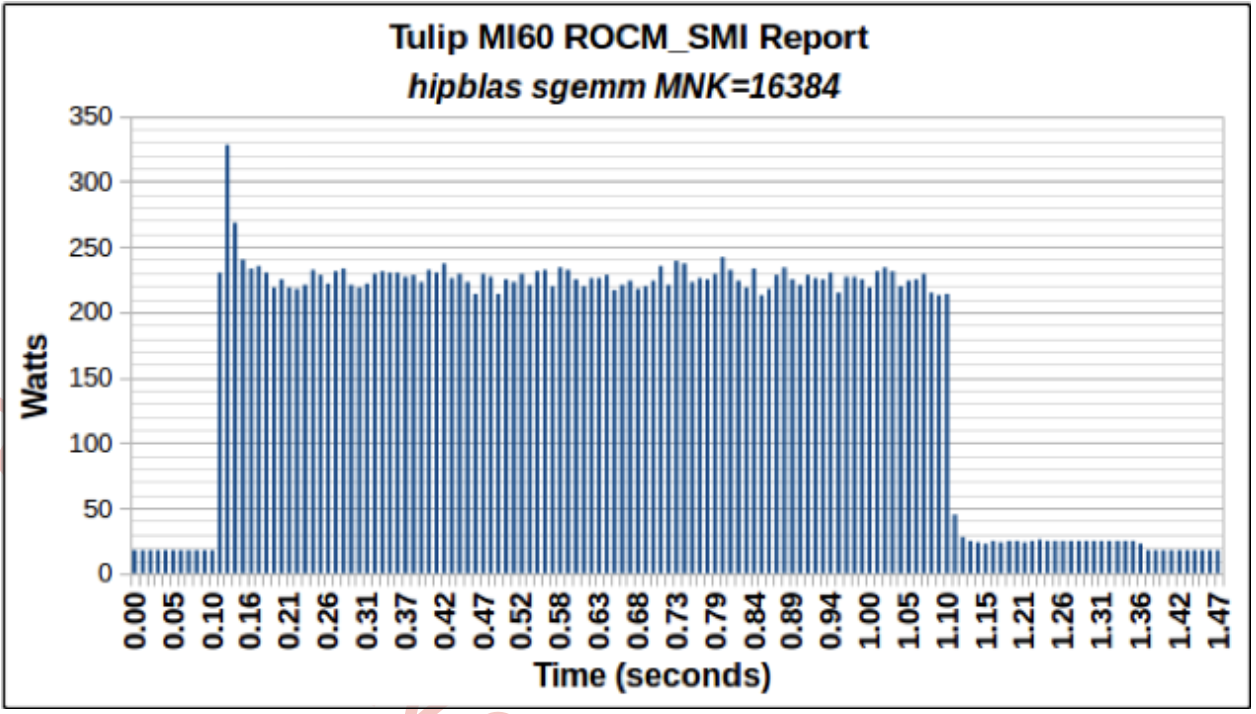
\includegraphics[width=0.9\linewidth]{FileAusiliari/Screenshots/Figure13-7.png}
    \caption{AMD MI60 GPU 上有 PAPI 的 SGEMM 的功耗。}
    \label{fig:PAPI7}
\end{figure}

Vampir 是一款商業工具,用於將事件日誌可視化為時間軸和統計圖表。事件日誌保留了每個事件的時間資訊,能夠幫助識別應用程式執行期間特性變化的性能問題。
Score-P 是一個高度可擴展且易於使用的工具套件,專為高效能計算(HPC)應用程式的性能分析與事件追蹤而設計。它是為 Vampir 生成事件日誌的首選方法。欲了解更多有關 Vampir 和 Score-P 的資訊,請參閱其用戶手冊,相關資料可在各自的官網上找到。
AMD ROCm 提供了完整的 AMD GPU 計算生態系統。除了完整的編譯與加速應用程式運行工具鏈外,ROCm 還提供了用於偵錯與性能分析的工具與 API。此外,ROCm 也提供 API 給外部工具,用於記錄應用程式的執行行為與性能指標。
Score-P 利用 AMD 的 rocProfiler 和 rocTracer 庫進行性能分析:
rocTracer 庫基於callback機制運行,工具會為特定事件註冊函式,這些事件會由 ROCm Runtime 觸發,包括 HIP API 函式的進入與退出、host與device間的數據傳輸、kernel啟動操作等。
rocProfiler 庫則用於定期採樣 GPU 的性能指標。
這些工具的結合能有效記錄應用程式運行時的行為與性能數據,便於進一步分析和優化。

\subsection{使用 Score-P 進行追蹤}

\begin{figure}
    \centering
    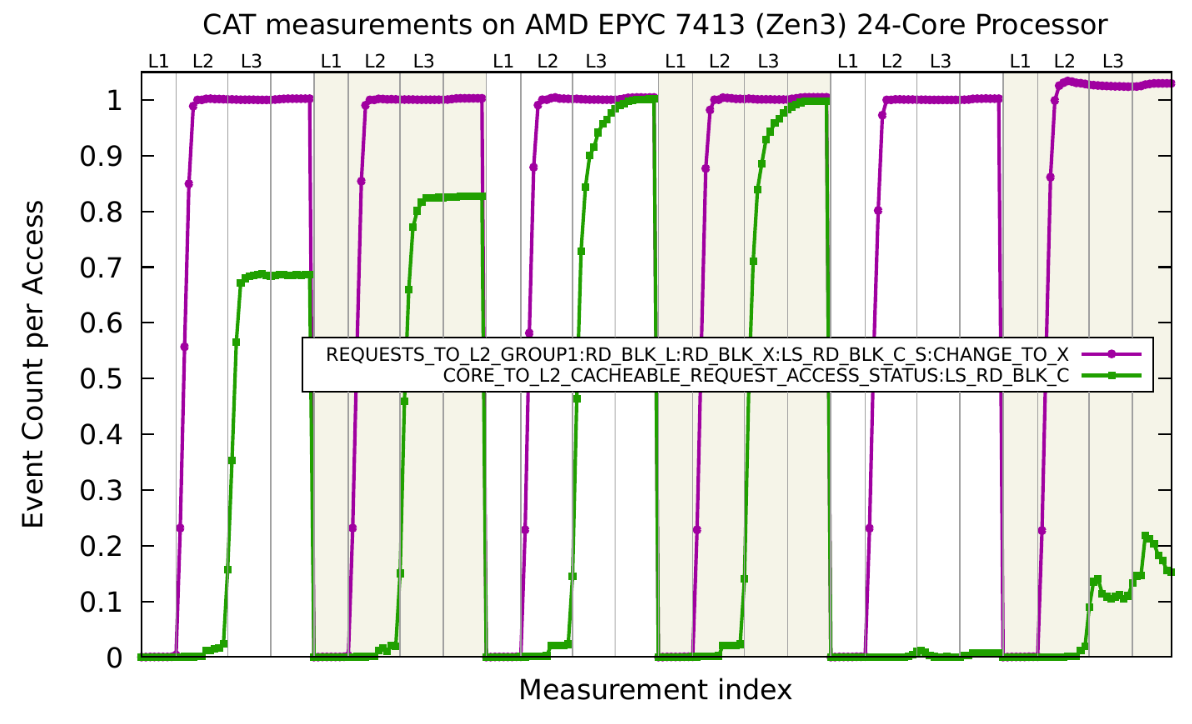
\includegraphics[width=0.9\linewidth]{FileAusiliari/Screenshots/Figure13-8.png}
    \caption{AMD MI60 GPU 上有 PAPI 的 SGEMM 的功耗。}
    \label{fig:PAPI8}
\end{figure}

在 Score-P 中,僅支援與高效能計算(HPC)相關的 ROCm tracer API 子集,並將這些的報告事件以 Open Trace Format (OTF) 版本 2(OTF2)形式呈現。生成的 OTF2 追蹤檔案可通過 Vampir 進行分析。

目前支援的事件涵蓋host與device之間的以下活動:

\begin{enumerate}
    \item Stream 管理:追蹤 GPU Stream 的創建、使用與銷毀。
    \item kernel啟動(Kernel launches):記錄 GPU kernel的啟動操作。
    \item host與device記憶體分配:監控記憶體分配和釋放的操作。
    \item host與device間的同步與非同步記憶體傳輸:包括數據在host與device之間的傳輸過程。
    \item device與 Stream 同步:記錄同步操作,確保host與device間的協調執行。
    \item host端的用戶自定義標記(Instrumentation):透過 rocTX 實現,用戶可以在host端自定義標記來追蹤應用程式執行中的關鍵事件。
\end{enumerate}


% 這些功能使得 Score-P 能夠詳細記錄 HPC 應用程式的運行行為,生成的 OTF2 文件為 Vampir 提供了深入分析應用性能和瓶頸的基礎。

大多數這些事件在 Score-P 中被映射為函式進入/退出事件,但某些事件包含額外資訊。Score-P 提供了正常的kernel名稱過濾功能,因此程式設計師可以提供過濾檔案以排除特定的kernel呼叫。記憶體分配則使用host與device的獨立分配指標進行追蹤,數據傳輸則是host與device之間的單向通信事件。

一組與 HIP 相關的 Score-P 環境變數允許程式設計師選擇記錄或忽略哪些類別的事件。預設情況下,所有事件都會被記錄。要採樣的指標列表也可以通過環境變數控制,並可使用由 rocProfiler 套件提供的 rocProf 工具進行查詢。

\begin{lstlisting}
$ rocprof --list-basic
$ rocprof --list-derived
\end{lstlisting}

\subsection{Score-P 用法}


Score-P 提供了一個命令,可在編譯/連結階段對應用程式進行Instrumentation。某些平行框架(例如 MPI 和 OpenMP)可以自動檢測,而某些則必須顯式啟用。要使用此功能,應用程式必須通過在所有編譯/連結命令前加上 Score-P 插桿器(scorep)來重新建構。
例如,原始命令為:
\begin{lstlisting}
$ gcc -c foo.o
\end{lstlisting}
需要改為:
\begin{lstlisting}
$ scorep gcc -c foo.o
\end{lstlisting}
同樣的操作適用於連結命令。

ROCm 基於 tracer 的插桿通過將 --hip 選項傳遞給 Score-P 插桿器(scorep)來啟用,其方式與啟用 CUDA 或其他加速器模式的Instrumentation相同。scorep-hipcc 編譯器封裝器會自動傳遞此標誌。更多有關使用 ROCm 插桿的詳細範例,請參閱 Score-P 文檔。

\subsection{分析 \Quicksilver 應用程式}
接下來,我們展示在執行 Quicksilver CORAL 基準應用程式時使用 Score-P 和 Vampir 的範例。Quicksilver 基準應用程式是一個 Monte Carlo Transport Code 的代理應用程式,屬於 Lawrence Livermore National Laboratory (LLNL) 的 Mercury 協同設計的一部分。我們的範例使用了支援 ROCm 的 Quicksilver 版本,該版本位於 GitHub 儲存庫的 AMD-HIP 分支中。

\subsubsection{流程}
首先,我們複製 Quicksilver 儲存庫並檢出 AMD-HIP 分支:
\begin{lstlisting}
$ git clone -b AMD-HIP \
      https:∕∕github.com∕LLNL∕Quicksilver.git
$ cd Quicksilver∕src
\end{lstlisting}

接下來,啟用 Score-P 插桿,建置該基準應用程式。為了讓 Score-P 插桿器(scorep-hipcc)正常運行,標準建置流程需要進行一些修改。以下是編譯與連結的步驟:

\begin{lstlisting}
$ sed -i -e 's,^CXX = $(HIP)∕bin∕,CXX = scorep-,' Makefile
$ make HIP=∕opt∕rocm
\end{lstlisting}



這個流程會生成名為 qs 的可執行檔,該檔案指定了一個適合此演示的輸入大小。應用程式以單個進程和一個 AMD GPU 運行,我們通過生成 OTF2 追蹤檔來收集性能數據:
\begin{lstlisting}
$ SCOREP_ENABLE_TRACING=true \
  SCOREP_TOTAL_MEMORY=4G \
  SCOREP_EXPERIMENT_DIRECTORY=Quicksilver-1x1-Instrumented \
  .∕qs
\end{lstlisting}

生成的追蹤檔位於 Quicksilver-1x1-Instrumented 中,現在可以通過 Vampir 開啟進行分析。圖 13.9 展示了host進程與加速器stream RocM[0:0] 的主時間軸。該格式與 CUDA 追蹤中使用的格式相同,包括加速器stream的命名,其中括號中的數字表示device和stream的 ID。此外,該圖在 "counter timelines" 的下方部分展示了host與device的記憶體分配指標。host初始化階段可以輕鬆識別,在此階段會分配host記憶體。同樣,也可以識別device初始化階段的記憶體分配過程。

\begin{figure}
    \centering
    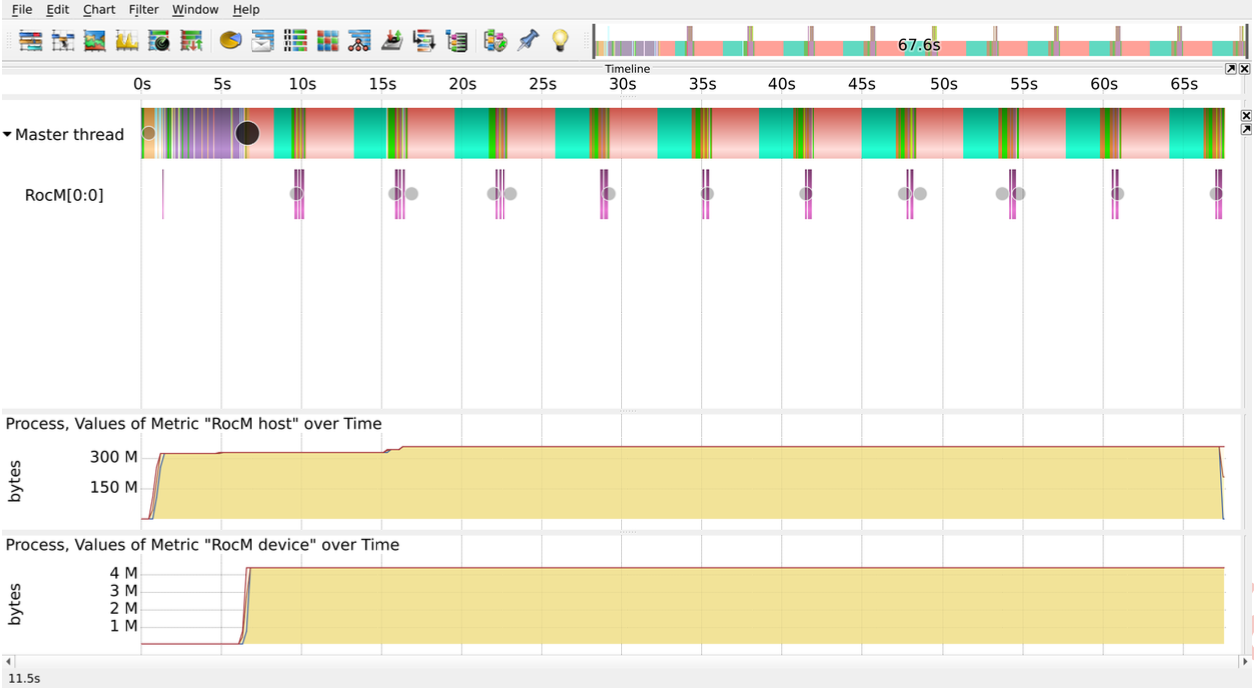
\includegraphics[width=0.9\linewidth]{FileAusiliari/Screenshots/Figure13-9.png}
    \caption{主時間軸顯示host和裝置記憶體使用率。}
    \label{fig:PAPI9}
\end{figure}


在 圖 13.10 中,我們展示了初始化階段的剖析結果,包括不同持續時間和大小的數據傳輸。所有 Quicksilver 的數據傳輸都是同步的,因此這些階段可以進行重疊處理以提高性能。
\begin{figure}
    \centering
    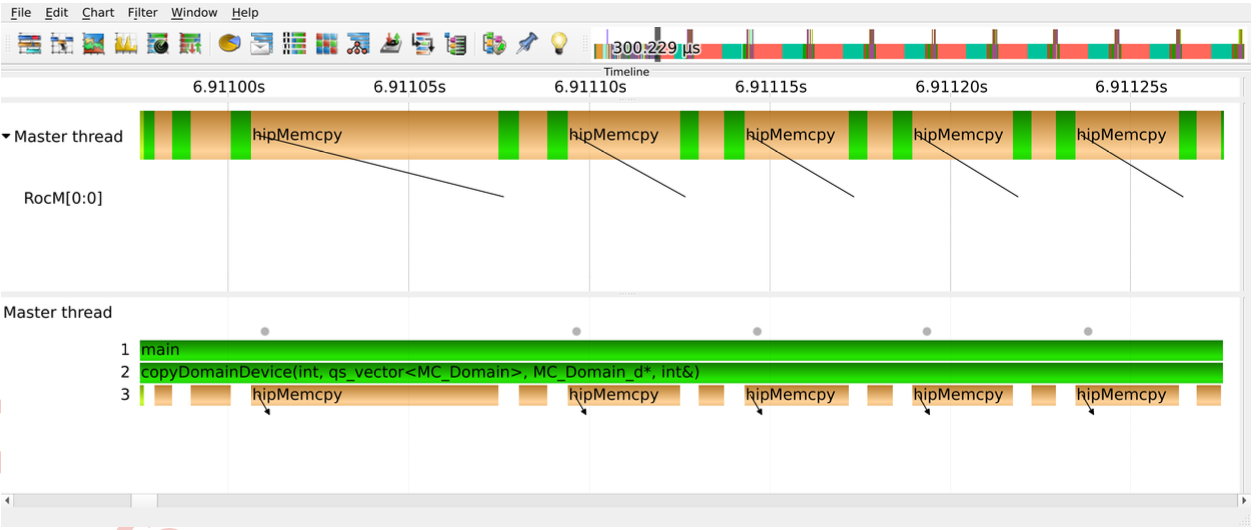
\includegraphics[width=0.9\linewidth]{FileAusiliari/Screenshots/Figure13-10.png}
    \caption{host/裝置傳輸的主控和進程時間軸。}
    \label{fig:PAPI10}
\end{figure}

圖 13.11 提供了device記憶體分配的快照,並包含主時間軸,顯示數據傳輸發生的時間(以黑色圓圈標示)。這清楚地展示了分配/填充週期的模式。

最後,圖 13.12 展示了主要計算階段,其中涉及單次kernel啟動的執行以及隨後的device同步以等待結果。追蹤顯示,對於 Quicksilver 而言,大部分kernel執行期間 CPU 處於空閒狀態,遵循 啟動–同步–複製結果 的模式。

\begin{figure}
    \centering
    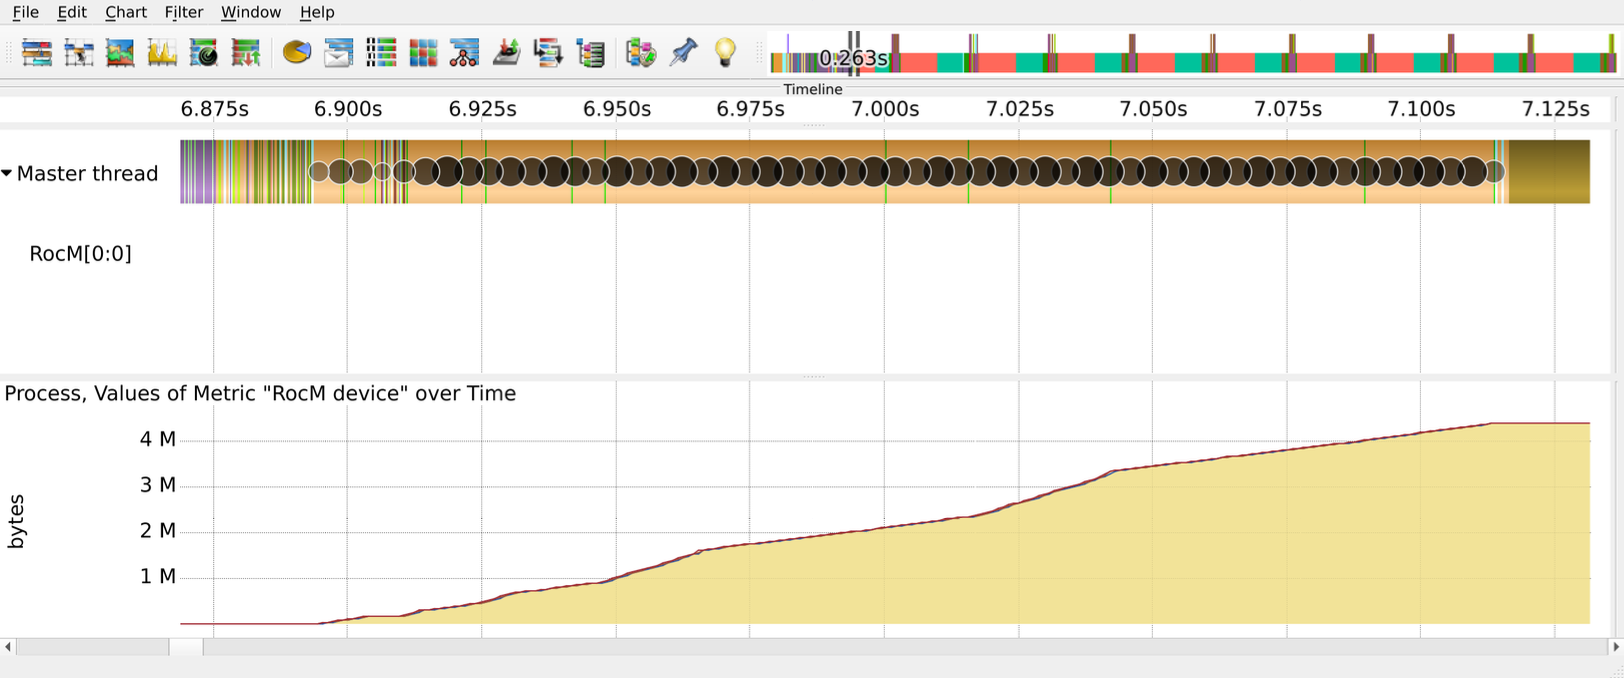
\includegraphics[width=0.9\linewidth]{FileAusiliari/Screenshots/Figure13-11.png}
    \caption{主時間軸顯示device記憶體利用率。}
    \label{fig:PAPI11}
\end{figure}

\begin{figure}
    \centering
    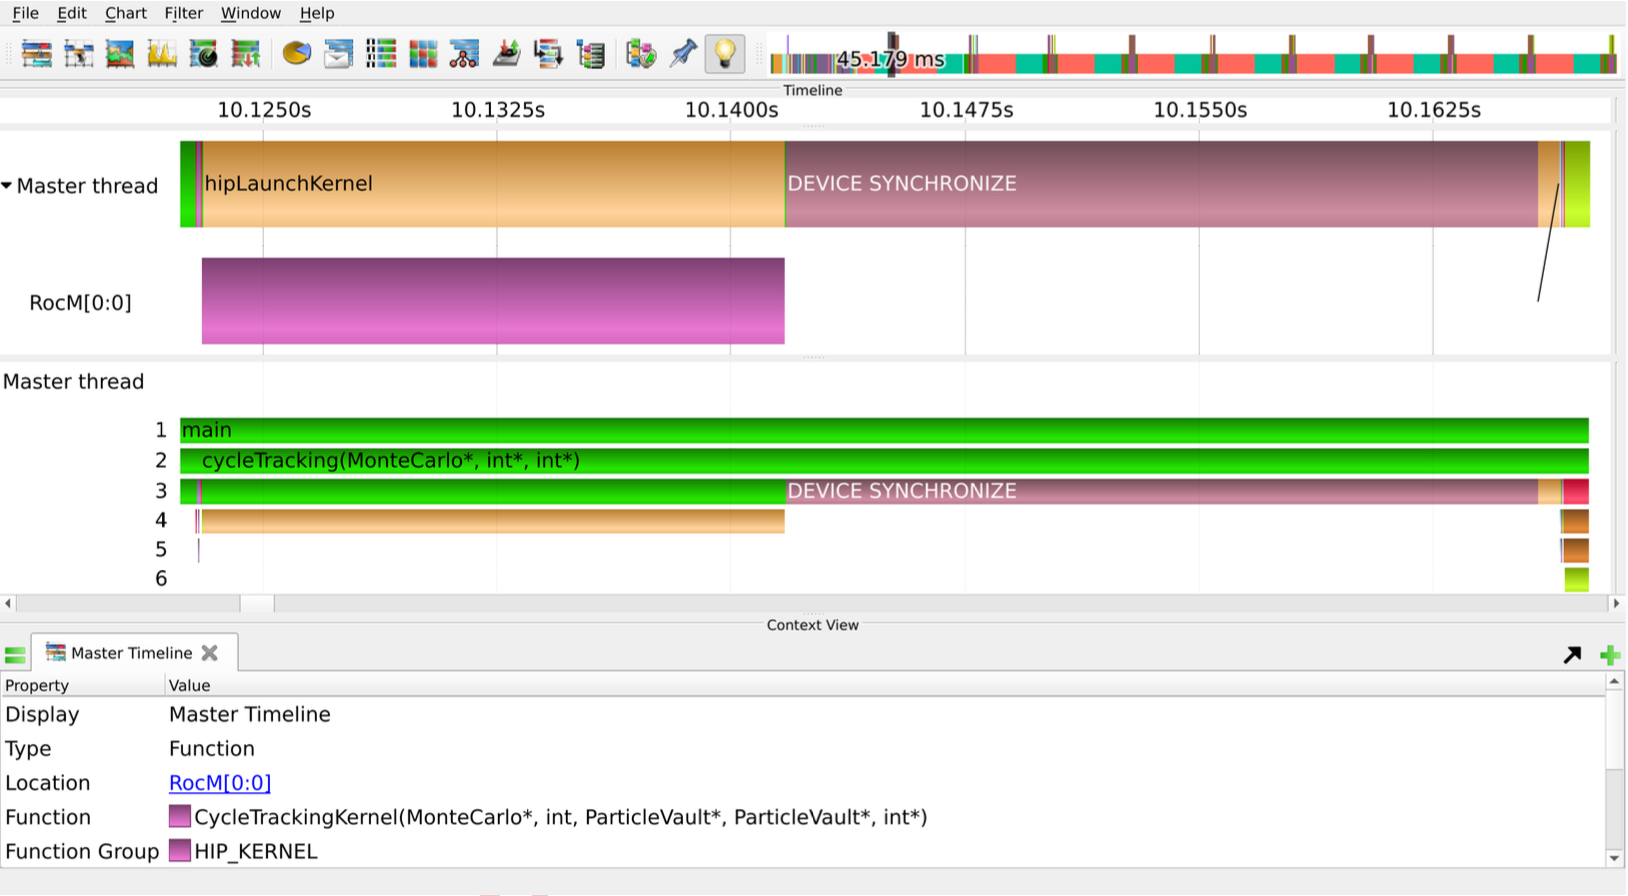
\includegraphics[width=0.9\linewidth]{FileAusiliari/Screenshots/Figure13-12.png}
    \caption{有kernel launch和裝置同步化的主要時間軸。}
    \label{fig:PAPI12}
\end{figure}

\subsubsection{總結}
Vampir/Score-P 生態系統全面支援 HIP/ROCm 的性能分析。我們提供了一個概述,並通過 Quicksilver 應用程式展示了它們的實用性。Vampir/Score-P 工具允許使用者對 ROCm 行為進行剖析,並支持利用平行框架(包括 MPI 和 OpenMP)的應用程式的性能分析。


\section{Trace Compass 與 Theia}
\subsubsection{Trace Compass}

Trace Compass 是一款用於多種追蹤格式的可視化和分析工具。追蹤分析需要經歷以下幾個步驟:

\begin{enumerate}
    \item 事件處理與狀態建模
每個事件會被傳遞到一個或多個分析模組,用於建模系統的狀態(例如,進程與執行緒表、每個執行緒的狀態以及 GPU 計算kernel)。例如,process\_create 事件會向進程表新增一個進程和執行緒,而排程事件會基於相關kernel更新當前與即將執行的執行緒狀態。整個追蹤期間所建模狀態的數據庫稱為「狀態歷史」。
    \item 跨節點追蹤同步
來自不同節點的追蹤(例如積極交換網路封包的節點)可以通過匹配不同節點的發送與接收事件來同步,並計算時鐘漂移與偏移量。
    \item 事件內容與高層次視圖
個別事件的內容可以顯示為詳細的事件列表,而更高層次的視圖與分析通常會查詢「狀態歷史」數據庫,以便快速導航追蹤資料。
    
\end{enumerate}

接下來的部分將介紹 Trace Compass 支援的兩種 HPC 追蹤格式及其相關案例研究。其他進階功能還包括:同步從不同節點收集的追蹤資料。計算分散式程式執行的關鍵路徑。提供所有視圖的時間同步,便於進一步分析分散式應用程式的性能問題。

\subsubsection{Theia}
Theia 是一個開放且可擴展的雲端和桌面整合開發環境(IDE)平台。它類似於 Visual Studio,並使用許多相同的基礎模組、協議和擴展 API。Theia 的圖形使用者介面(GUI)與 Visual Studio 類似,對多種程式語言的支援透過 語言伺服器協議(LSP) 委派給外部模組。因此,通過 LLVM 的 clangd 語言伺服器,Theia 編輯器不僅支援 C/C++,還支援多種相關語言,如 OpenCL。此外,Theia 透過 除錯器適配器協議(DAP) 與 GDB 通信,提供進階除錯功能。

Trace Compass 被重建為將其 GUI 前端與追蹤讀取和分析後端分離。後端伺服器現在可以透過 Eclipse 提供其經典的 GUI 前端,也可以介接 Theia。為了連接後端與 Theia,開發了 追蹤伺服器協議(TSP),其功能類似於 LSP 和 DAP。TSP 使得 theia-trace-extension 插件能與 Theia 整合,這樣用戶就可以直接在 Theia IDE 中分析這些追蹤資料。此整合使得 Theia 不僅能進行程式碼開發和除錯,還能直接執行追蹤資料的分析,提供了一個全面的 HPC 分析與開發平台。

\subsubsection{通用追蹤格式Common Trace Format (CTF)}
CTF (Common Trace Format) 是一種二進位追蹤格式,設計目的是將追蹤開銷降到最低。它具有通用性,允許程式設計師定義自己的事件類型,其有效負載格式則定義於一個元數據檔案中。該元數據檔案在解析時會將追蹤內容轉換為高階表示。

CTF 提供了一個插件,支援使用 ROCm 的 GPU 追蹤程式,並結合 rocProfiler 和 rocTracer。該插件使用優先隊列對 HIP 和 HSA 事件按發生順序進行排序,然後利用 barectf 將它們寫入 CTF stream中。生成的追蹤資料可以通過 Trace Compass 進行分析和可視化顯示。

\subsubsection{OTF2}
OTF2 [61, 28] 是一種常見的二進位追蹤格式,用於追蹤大規模平行計算系統。這類追蹤通常會生成大量的追蹤檔案,有時會達到數百 GB 或甚至 TB 的數據量。然而,OTF2 經過優化,可生成緊湊且高效的結果 [81]。

要生成 CTF 格式的 ROCm 追蹤:
從 GitHub 網站下載 rocProfiler 和 rocTracer 插件:
\begin{lstlisting}
https://github.com/dorsal-lab/rocprofiler\_ctf\_plugin
\end{lstlisting}

安裝後,按照以下步驟生成 CTF 格式的追蹤:
使用 CTF\_PLUGIN 環境變數匯出插件路徑:
\begin{lstlisting}
$ export CTF_PLUGIN=∕path∕to∕plugin.
\end{lstlisting}

使用 rocprof 命令,並帶上 --ctf-format 和 -d 選項指定追蹤目錄:
\begin{lstlisting}
rocprof --ctf-format --hip-trace -d /path/to/my/trace ./my_program
\end{lstlisting}

如果插件版本為 "rocm-4.2.x-interval"、"rocm-4.3.x" 或更高,運行以下命令進行後處理:
\begin{lstlisting}
python $CTF_PLUGIN/scripts/post_processing.py /path/to/my/trace
\end{lstlisting}

您的追蹤文件現在位於 CTF\_trace 目錄中,具體位置在 -d 選項所指定的子目錄內。


要生成 OTF2 格式的追蹤,請按照以下步驟操作:
安裝 Score-P 和 OTF2:
\begin{lstlisting}
https://www.vi-hps.org/projects/score-p/
\end{lstlisting}

安裝 OTF2-to-CTF 轉換器:
\begin{lstlisting}
https://github.com/dorsal-lab/OTF2-to-CTF-converter
\end{lstlisting}

以 OTF2 格式追蹤程式:
使用 Score-P 編譯程式。
啟用追蹤功能:
\begin{lstlisting}
$ export SCOREP_ENABLE_TRACING=1
\end{lstlisting}
執行已編譯的程式,生成包含 OTF2 追蹤的 scorep-<identifier> 目錄。

將 OTF2 追蹤轉換為 CTF:
將轉換器路徑匯出至 OTF2\_CONVERTER 環境變數:
\begin{lstlisting}
$ export OTF2_CONVERTER=/path/to/converter
\end{lstlisting}
使用以下命令進行轉換:
\begin{lstlisting}
$ OTF2_CONVERTER/otf2_converter ./path/scorep/trace/traces.otf2
\end{lstlisting}

現在,您應該可以在 converted\_otf2\_<identifier> 目錄中找到 CTF 追蹤。

範例追蹤與程式碼可在以下位置找到:
https://github.com/dorsal-lab/OTF2\_testcases


\subsubsection{Theia Trace Extension}
Theia Trace Extension 提供了開源版本,可直接構建或在 GitPod 上託管使用。儲存庫位置如下:
\begin{lstlisting}
https://github.com/theia-ide/theia-trace-extension
https://github.com/dorsal-lab/tracevizlab/tree/master/labs/304-rocm-traces
\end{lstlisting}

我們使用一個 ROCm 追蹤來展示此框架的功能。

\begin{figure}
    \centering
    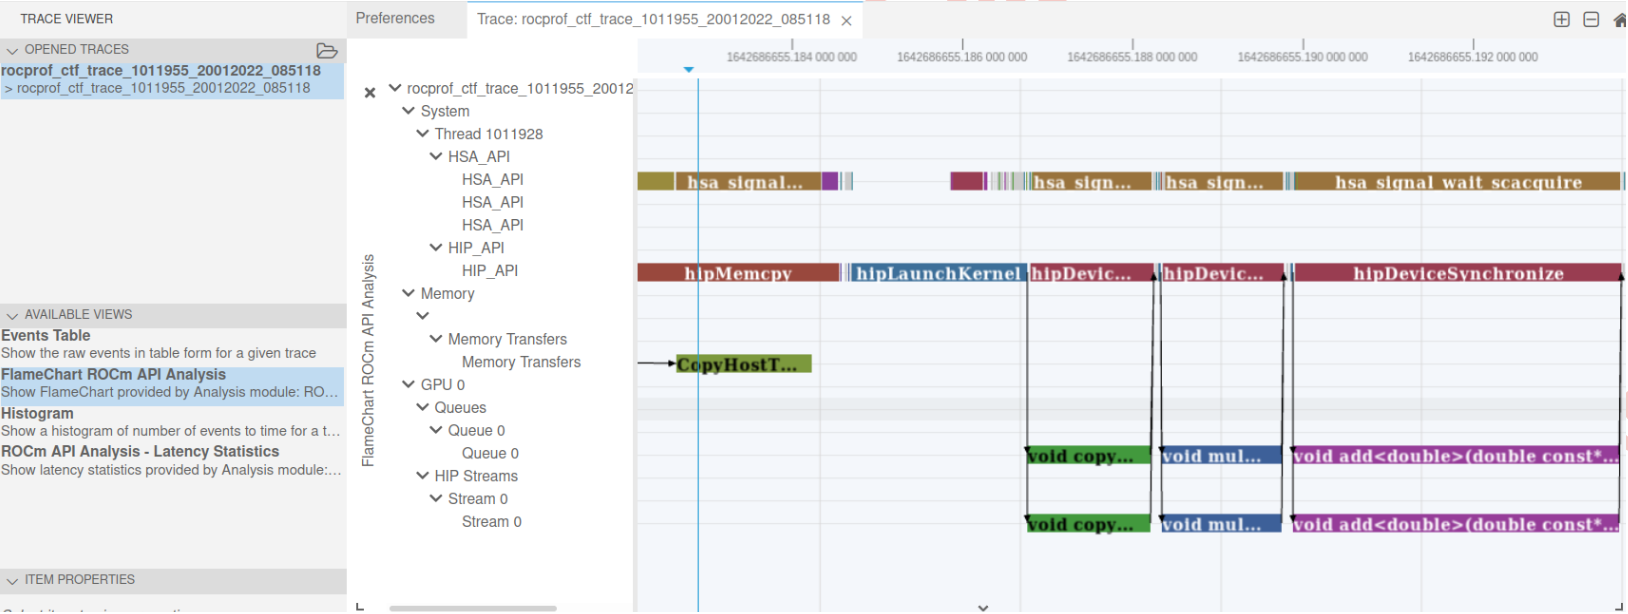
\includegraphics[width=0.9\linewidth]{FileAusiliari/Screenshots/Figure13-13.png}
    \caption{使用 Theia Trace Extension 進行視覺化。}
    \label{fig:PAPI13}
\end{figure}

圖 13.13 展示了一個 HIP 程式執行的詳細視圖。該程式的 add4 HIP kernel 來自 HIP-Examples [7] 儲存庫。此追蹤包含四個不同計算kernel連續執行的事件。在圖中:左上方的菜單顯示已打開的不同追蹤。中間左側顯示可用的分析。左下方顯示用戶選擇的詳細資訊。主視圖包含程式的火焰圖分析。

從上到下,我們可以看到系統執行緒按 API 類型(如 HIP 和 HSA)及記憶體傳輸進行分組。在底部,展示了 GPU kernel的執行情況。圖中的不同區域包括:每個隊列中的kernel執行。每個 HIP stream中的kernel執行。每個kernel被分配一種特定顏色,箭頭表示 HIP API 呼叫與實際 GPU kernel執行之間的依賴關係。需要注意的是,由於初始化過程發生在第一步,首次執行耗時較長。


\subsubsection{Theia.cpp debug extension}

\begin{figure}
    \centering
    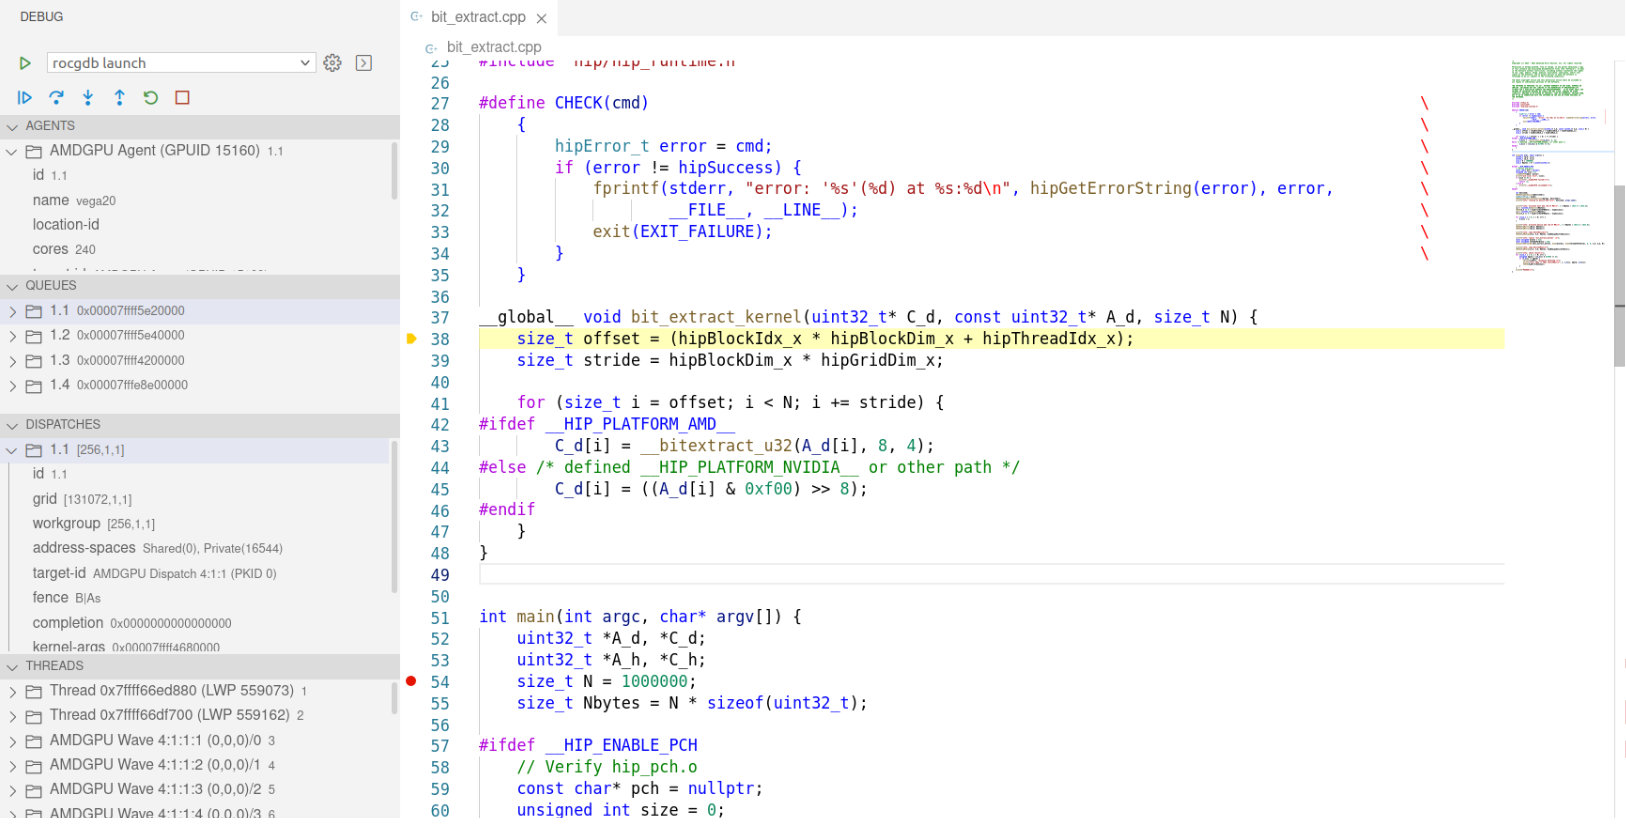
\includegraphics[width=0.9\linewidth]{FileAusiliari/Screenshots/Figure13-14.png}
    \caption{Theia 中的 rocgdb 偵錯視圖。}
    \label{fig:PAPI14}
\end{figure}

Theia.cpp Debug Extension 提供了一個用於 C/C++ 及相關程式語言的除錯視圖 [72]。它基於 DAP [55],並使用機器介面協議與 GDB 通信。由於 rocgdb 擴展了 GDB 的功能以支援 ROCm,該擴展處理了多個新指令,並顯示與 ROCm 相關的 GPU 資訊,例如隊列、代理、派遣和通道。

要使用 Theia.cpp Debug Extension,安裝後,在啟動程式時只需指定 GDB 參數。可以設置斷點來暫停程式執行,同時在 GPU 除錯視圖中存取 rocgdb 提供的資訊。


\subsubsection{Trace Compass}

\begin{figure}
    \centering
    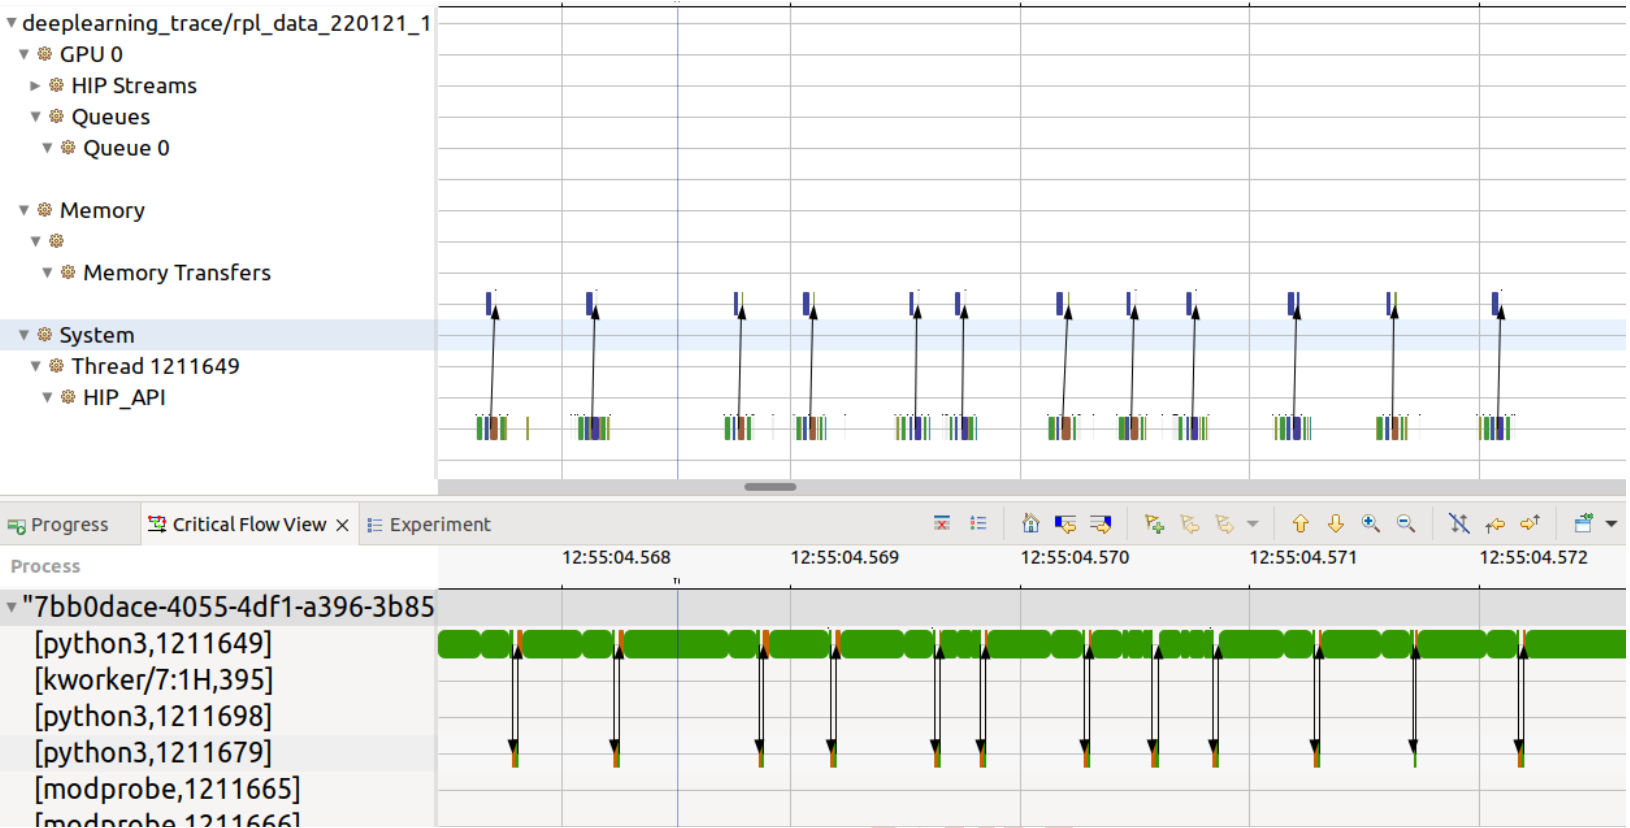
\includegraphics[width=0.9\linewidth]{FileAusiliari/Screenshots/Figure13-15.png}
    \caption{Trace Compass的多個同步追蹤。}
    \label{fig:PAPI15}
\end{figure}

在 圖 13.15 中,我們展示了一個深度學習程式的執行以及其 Linux kernel追蹤分析。為了生成 Linux kernel追蹤,我們使用了 Linux Trace Toolkit: Next Generation [50],並啟用了幾個追蹤點。追蹤器記錄了 Linux kernel事件,例如系統調用、記憶體分配和執行緒搶佔,這些對於偵錯多執行緒應用程式非常有用。僅依靠 GPU API 調用有時無法提供完整的資訊。在這種情況下,結合多種追蹤來源能讓程式設計師更緊密地追蹤程式行為。此處展示的分析與 Theia-trace-extension 部分相同,僅是使用了不同的前端來訪問相同的 Trace Compass 伺服器後端。

圖的底部顯示了“關鍵流程”視圖,展示了程式主執行緒的關鍵路徑。關鍵路徑分析從執行緒的末端開始,沿著依賴鏈向前回溯,根據資源爭用識別出最長路徑。因此,我們可以確定進程在何時必須等待信號量或 I/O 操作。在圖中,可以看到執行緒 1,211,649 和 1,211,698 之間的關係,其中前者必須等待後者完成一個操作。


\section{TAU}

TAU Performance System® [64] 是一套平行性能評估工具包,支援剖析和追蹤模式的測量。它可以應用於未修改的二進位檔,並識別應用程式執行時間的分佈以及其他系統資源的使用情況。TAU 是開源的,可在以下網址獲取:
http://tau.uoregon.edu

TAU 利用多種函式庫和技術的支援,例如:rocProfiler [73] 和 rocTracer [74] 用於 HIP/ROCm 測量。GNU binutils [31] 用於符號解析與解碼。PAPI [71] 用於硬體性能計數。OTF2 [27] 用於可擴展的分散式追蹤收集。
TAU 還利用平行程式設計模型的支援,整合函式庫和執行時環境的性能測量回調,支援的模型包括 MPI [30]、OpenMP [59]、OpenACC [58] 和 Kokkos [76]。當插桿或回調不可用時,TAU 會在 CPU 上進行定期採樣,通過中斷程式並捕獲計數器來生成統計剖析。收集樣本時,可選擇執行呼叫堆疊回溯以捕獲完整的樣本上下文。

對於缺乏傳統呼叫堆疊的程式設計模型(如 High Performance ParalleX [39]),或支援動態執行時適應的應用程式與函式庫,TAU 提供了一個替代方案,名為 Autonomous Performance Environment for eXascale (APEX) 測量函式庫 [36]。儘管 APEX 可用於剖析任何程式,其捕獲的性能數據是從任務依賴的角度呈現,而非呼叫堆疊。動態執行時適應由一個策略引擎提供,該引擎會定期或按需評估性能狀態,並應用策略規則調整控制參數。

\subsection{使用 TAU 分析 HIP program}

\begin{figure}
    \centering
    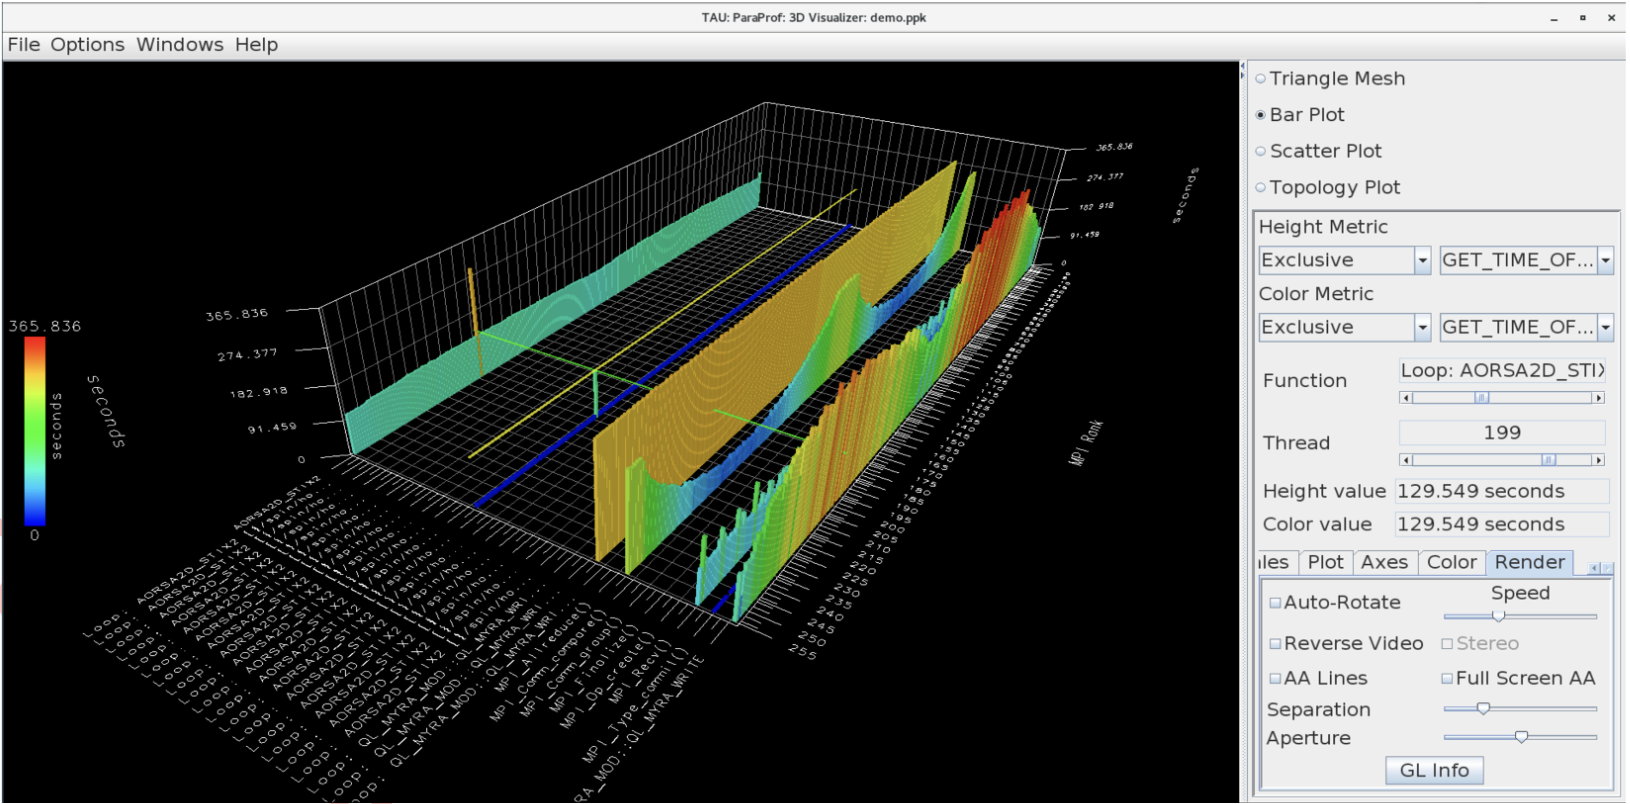
\includegraphics[width=0.9\linewidth]{FileAusiliari/Screenshots/Figure13-16.png}
    \caption{使用 TAU 的 ParaProf 工具進行 3D 視覺化,顯示輪廓形狀。}
    \label{fig:PAPI16}
\end{figure}

TAU 支援使用 rocProfiler 和 rocTracer APIs 對 HIP 程式進行剖析與追蹤。除了 rocProfiler 提供的事件外,rocTracer 還為 HIP 和 HSA 執行時系統事件提供了 TAU 插桿功能。為生成性能數據,用戶通常使用 tauexec 工具啟動應用程式。

TAU 通過第三方函式庫進行安裝,例如:binutils 和 libdwarf [20]:將程式計數器值轉換為原始碼位置信息(例如,檔名、函式名和行號)。libunwind:回溯系統呼叫堆疊。OTF2:生成 OTF 格式追蹤檔案。
TAU 提供自動下載選項,可根據需要使用正確的標誌(如 -fPIC)安裝這些函式庫以生成位置獨立的程式碼。

以下展示了一個典型的 TAU 安裝配置:
\begin{lstlisting}
.∕configure -rocm=<dir> -rocprofiler=<dir> \
-bfd=download -unwind=download -dwarf=download
-otf=download \
-iowrapper ...
make install
\end{lstlisting}

此配置生成了 tauexec 工具,使用帶有 -rocm 和 -rocprofiler 標籤的上述配置來啟動應用程式,具體使用如下:

\begin{lstlisting}
tau_exec -T rocm,serial,rocprofiler -ebs -rocm .∕a.out
\end{lstlisting}


\begin{figure}
    \centering
    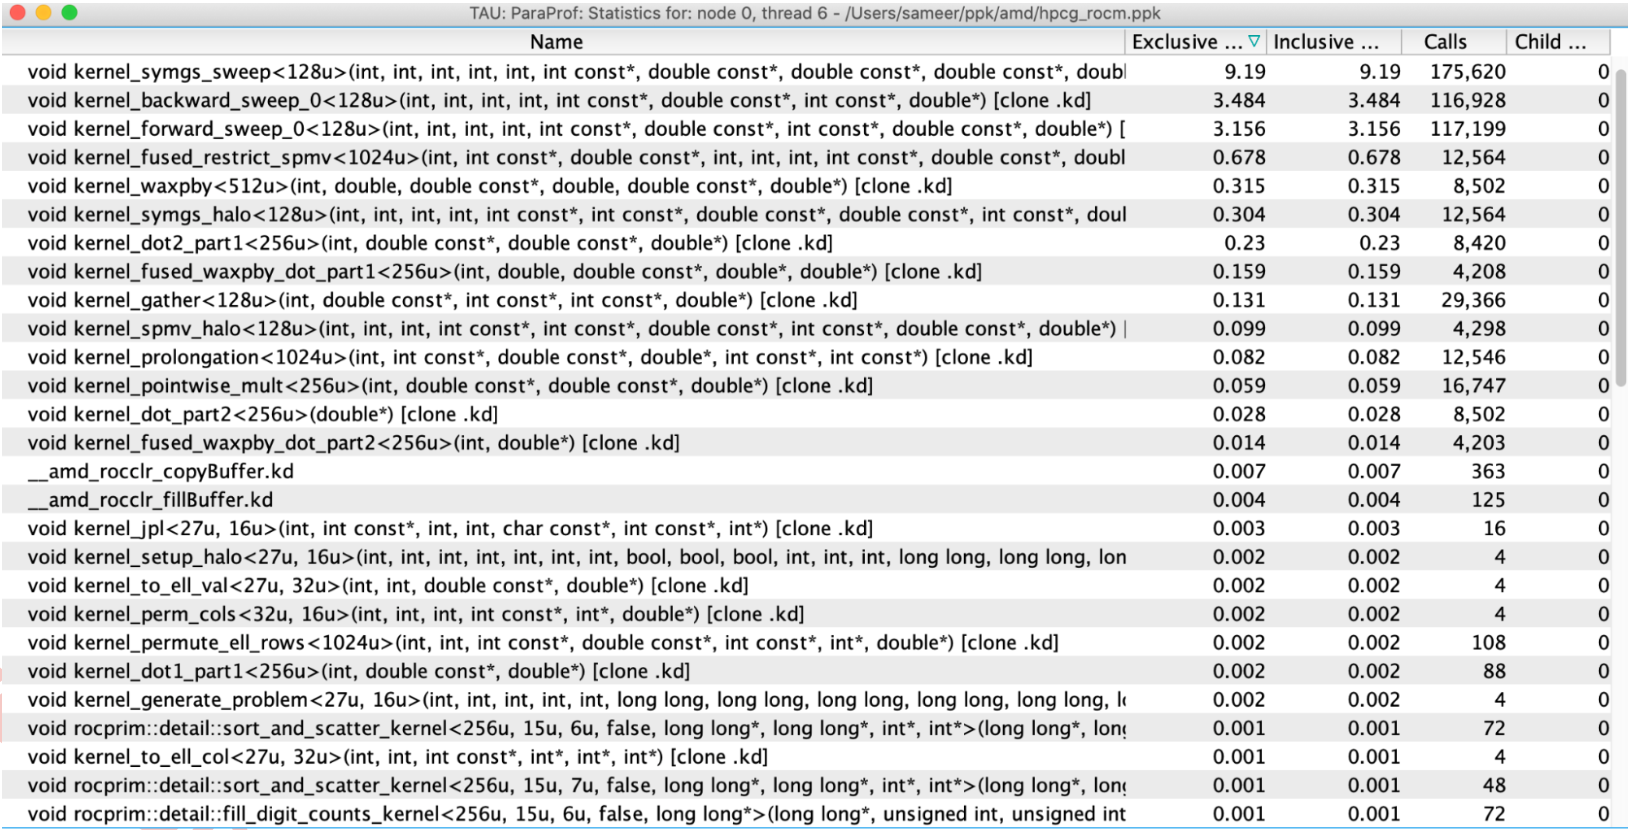
\includegraphics[width=0.9\linewidth]{FileAusiliari/Screenshots/Figure13-17.png}
    \caption{來自 rochpcg 應用程式的內核事件,如 TAU 的 ParaProf 設定檔瀏覽器中所示。}
    \label{fig:PAPI17}
\end{figure}

當 MPI 未為 TAU 配置時,執行時會選擇序列化的配置標籤。通過 tauexec 啟動時,TAU 會預加載 TAU 動態共享對象到正在執行的應用程式的位址空間,生成回調並攔截系統調用。可選地,當使用 -ebs 選項時,TAU 會使用事件驅動的採樣(EBS)定期中斷應用程式,並生成與原始碼位置對應的詳細剖析數據。通過 rocProfiler 和 rocTracer APIs 的回調,TAU 收集 GPU 上執行kernel的時間戳資訊以及數據傳輸資訊。

然而,時間戳對可能無序,這對於生成需要單調遞增系統時間戳的追蹤檔案構成挑戰。同時,GPU 時間戳還需要與 CPU 時間戳相關聯,以生成一致的全局性能數據視圖。TAU 使用一種新穎的滑動窗口演算法來緩衝kernel時間戳對,並在緩衝區滿時將它們寫入磁碟。通過延遲提交追蹤數據,系統可以處理無序的kernel時間戳。目前滑動窗口大小通過試錯選擇為 128K 對啟動/停止kernel執行事件。記錄在剖析檔案中的kernel事件會為每個隊列保存到單獨的執行執緒中。

圖 13.17 顯示了在 ParaProf 工具中 rochpcg 應用程式的某個隊列中每個kernel的耗時。TAU 支援通過 EBS 進行 CPU 和 GPU 的剖析。執行於 CPU 上的程式碼區域可以通過性能插桿進行高亮顯示,無需重新編譯程式碼。圖 13.18 顯示了在 Quantum Monte Carlo Package (QMCPack) 應用程式中,執行於多個執行緒上的 computeDistance 方法的耗時。在此,我們可以觀察應用程式區域在多執行緒的 CPU 端的表現。

需要注意的是,單個kernel的執行可能會在多個 GPU 上進行追蹤,如 圖 13.19 所示。儘管這些二維顯示資訊豐富,TAU 的 ParaProf 剖析瀏覽器還包含了一個 3D 可視化工具,展示了映射到執行緒(階層)和函式的代碼區域中專用耗時的互動式 3D 視圖,使用戶能夠查看剖析形態。圖 13.16 顯示了一個 3D 視窗,其中十字線表示函式,滑塊表示執行緒,用戶可以準確定位單個執行緒。


\subsection{使用 TAU 追蹤 HIP program}


\begin{figure}
    \centering
    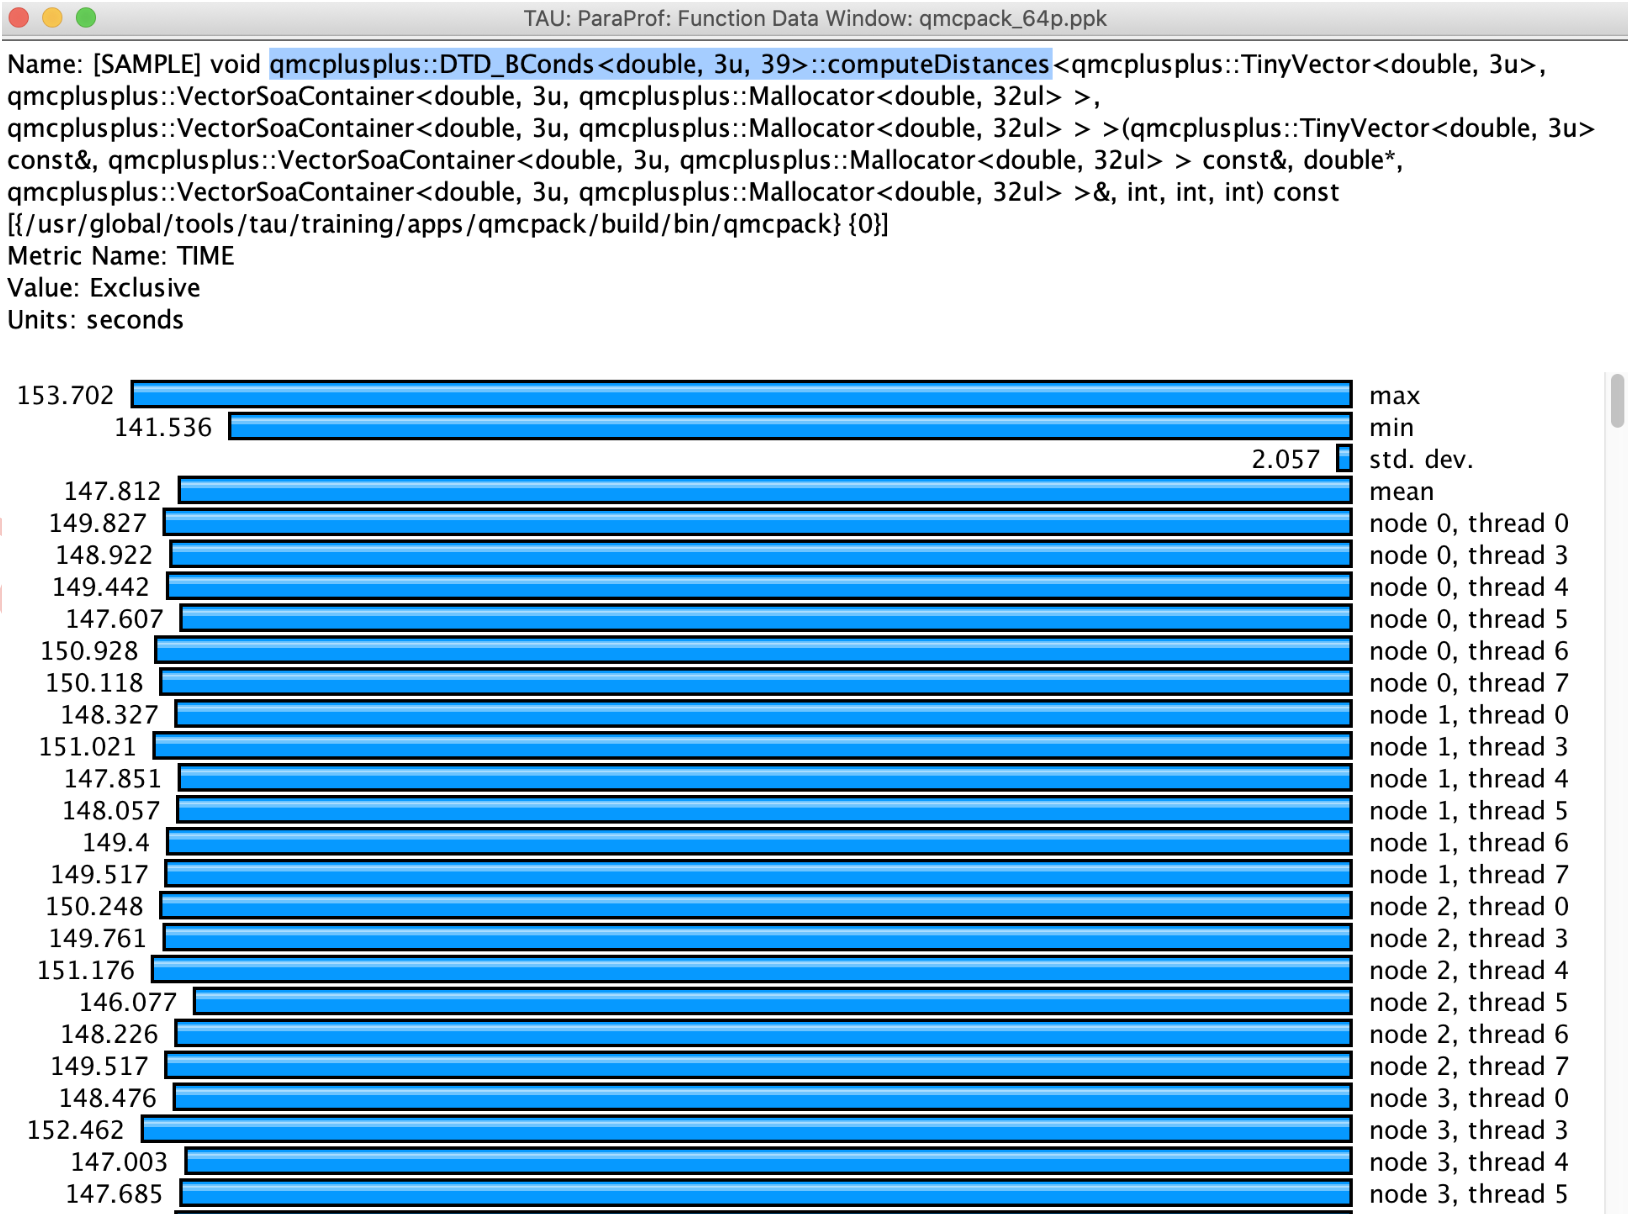
\includegraphics[width=0.9\linewidth]{FileAusiliari/Screenshots/Figure13-18.png}
    \caption{應用於 QMCPack 的 EBS 有助於精確定位計算成本高的程式碼區域。}
    \label{fig:PAPI18}
\end{figure}

\begin{figure}
    \centering
    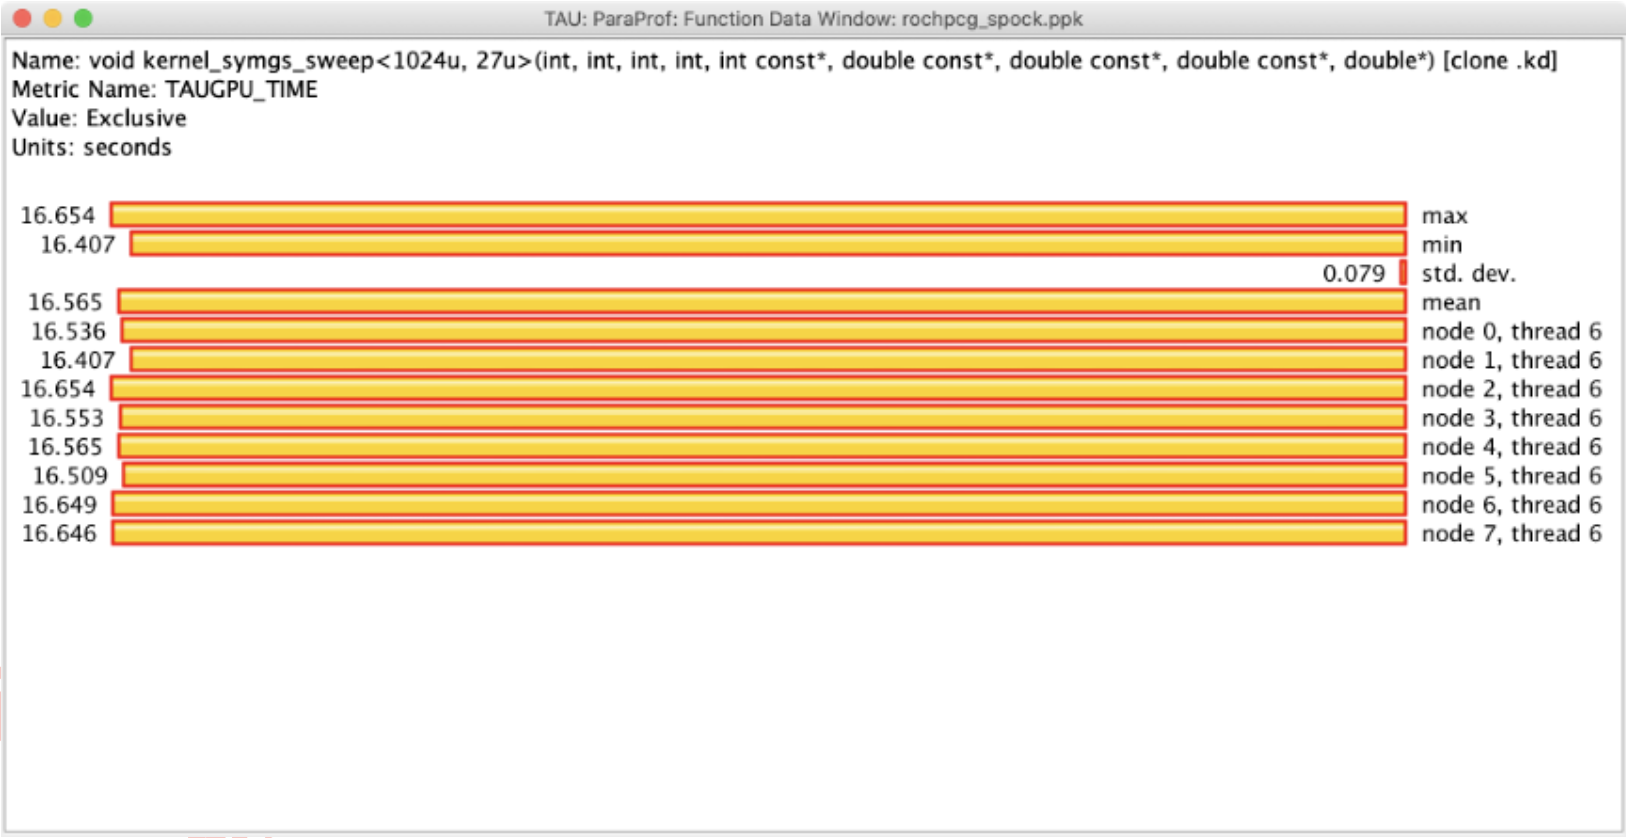
\includegraphics[width=0.9\linewidth]{FileAusiliari/Screenshots/Figure13-19.png}
    \caption{TAU 的 ParaProf 工具顯示單一kernel在多個 GPU 佇列中的執行情況。}
    \label{fig:PAPI19}
\end{figure}

雖然剖析提供了匯總統計資料(例如,多次調用kernel的總執行時間),但追蹤能夠突出時間上的變化。TAU 生成的追蹤檔案既可以是其原生的 TAU 格式,也可以是 OTF2 格式。以 TAU 格式生成的追蹤可以合併並轉換為 Jumpshot 的 SLOG2 格式以及 JSON 格式,以便通過 Google Chrome 的 chrome://tracing 或 Perfetto trace browser [32] 進行可視化。

TAU 還支援 Kokkos [76, 63] 的剖析介面,該介面提供了一種性能可移植的方法,使用 C++ Lambda 函式來表達應用程式中的平行操作,例如 for、scan 和 reduce 操作。這些 Lambda 函式內部會轉換為 GPU 後端(例如 HIP)。這些平行操作的第一個參數是一個可選的字元串,用於表示有意義的原始碼結構。TAU 與 Kokkos 介接,跟蹤這些高階抽象並將kernel執行映射到它們上。在缺乏用戶註解的情況下,使用模板實例化來進行跟蹤。

圖 13.22 展示了在 T.U. Dresden 的 Vampir 追蹤可視化工具中kernel執行的時間軸顯示。通過 TAU 的 OTF2 追蹤生成功能,在使用 tauexec 和相應的命令(如 export TAU\_TRACE=1 或 export TAU\_TRACE\_FORMAT=otf2)啟動未修改的程式碼後,追蹤檔案無需進行處理(例如合併或轉換)。


\subsection{使用 APEX 衡量 HIP program}

\begin{figure}
    \centering
    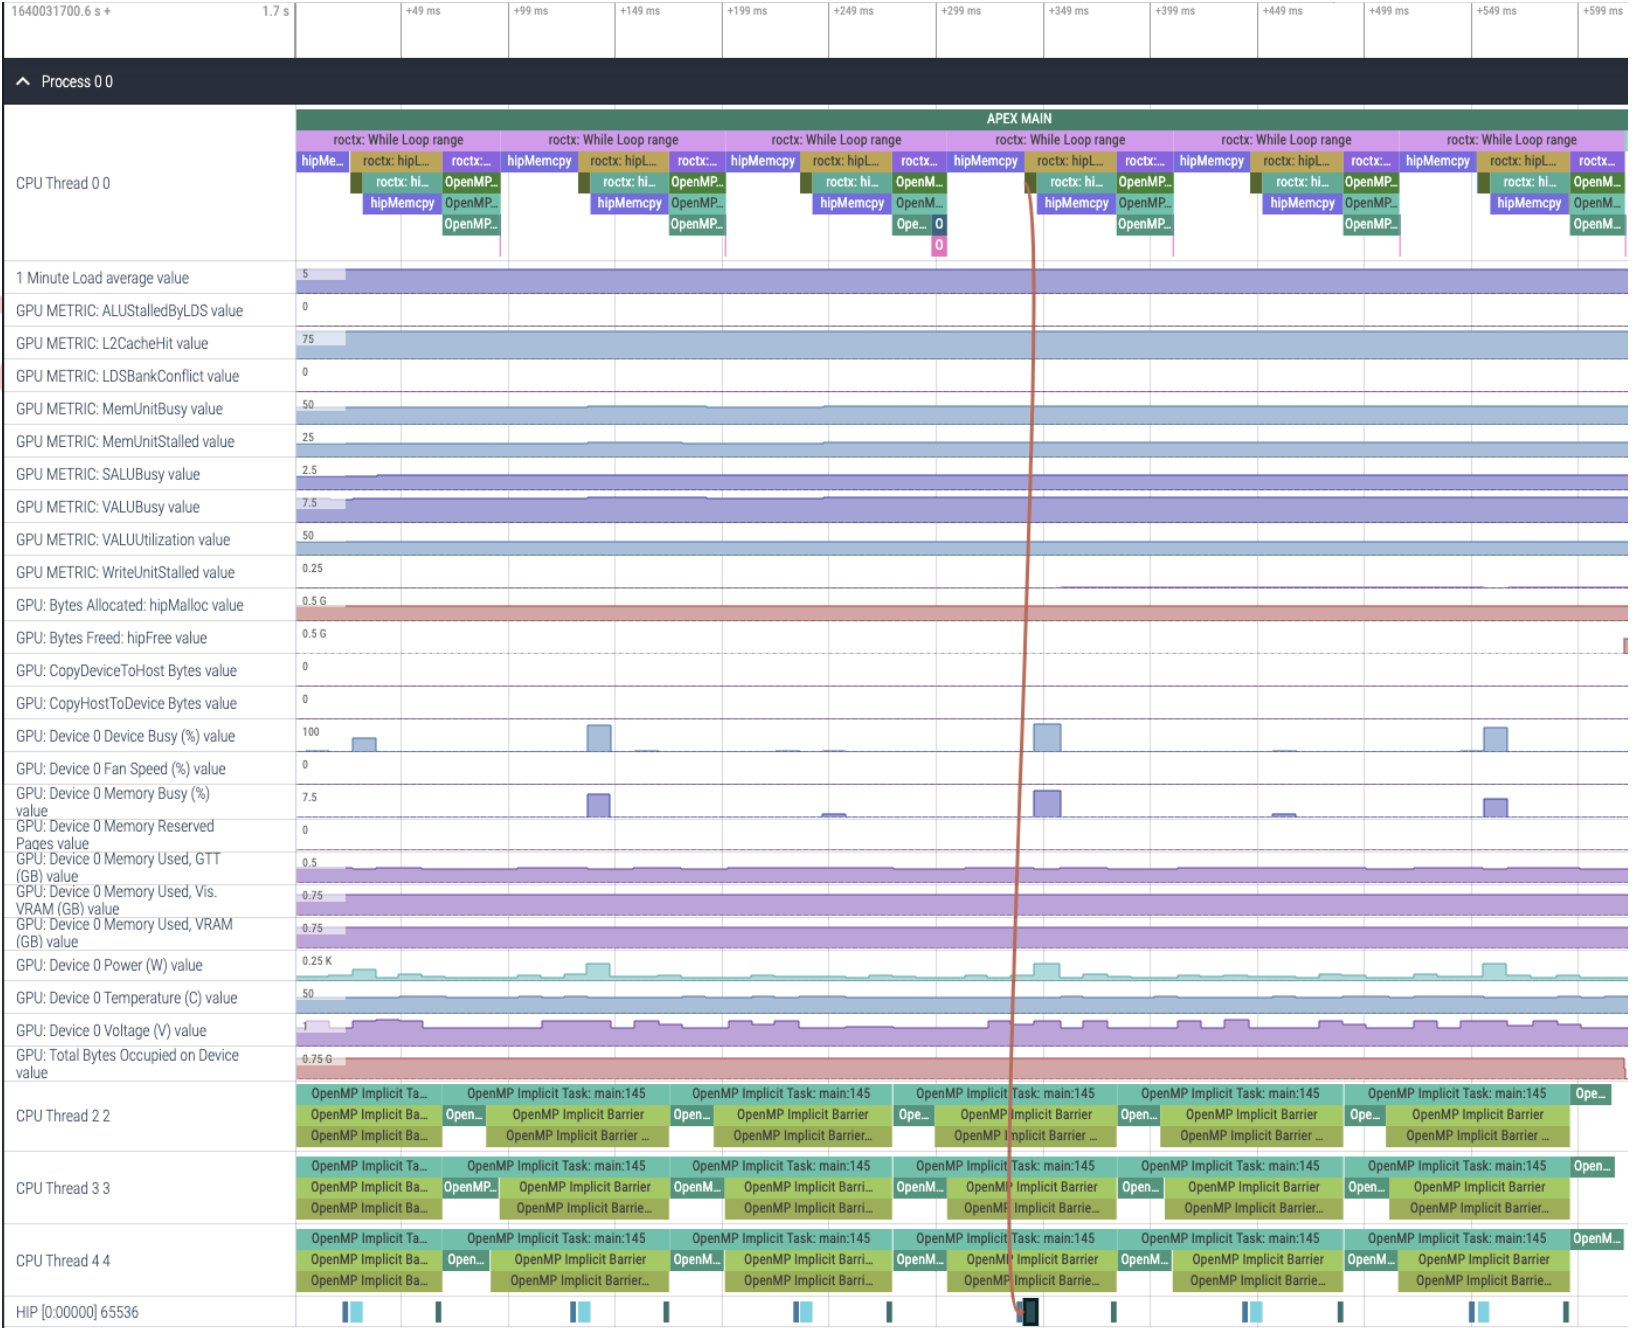
\includegraphics[width=0.9\linewidth]{FileAusiliari/Screenshots/Figure13-20.png}
    \caption{APEX 任務依賴樹由 Perfetto 渲染。在此範例中,第一個 CPU 執行緒位於追蹤的頂部,工作 CPU 執行緒位於底部,而 HIP GPU 活動則位於三個工作執行緒的下方。APEX 還捕捉了 ROCTX 插桿調用與標記。紅色箭頭突出顯示的stream事件表示從 HIP API 調用到 GPU device活動的控制stream。}
    \label{fig:PAPI20}
\end{figure}

\begin{figure}
    \centering
    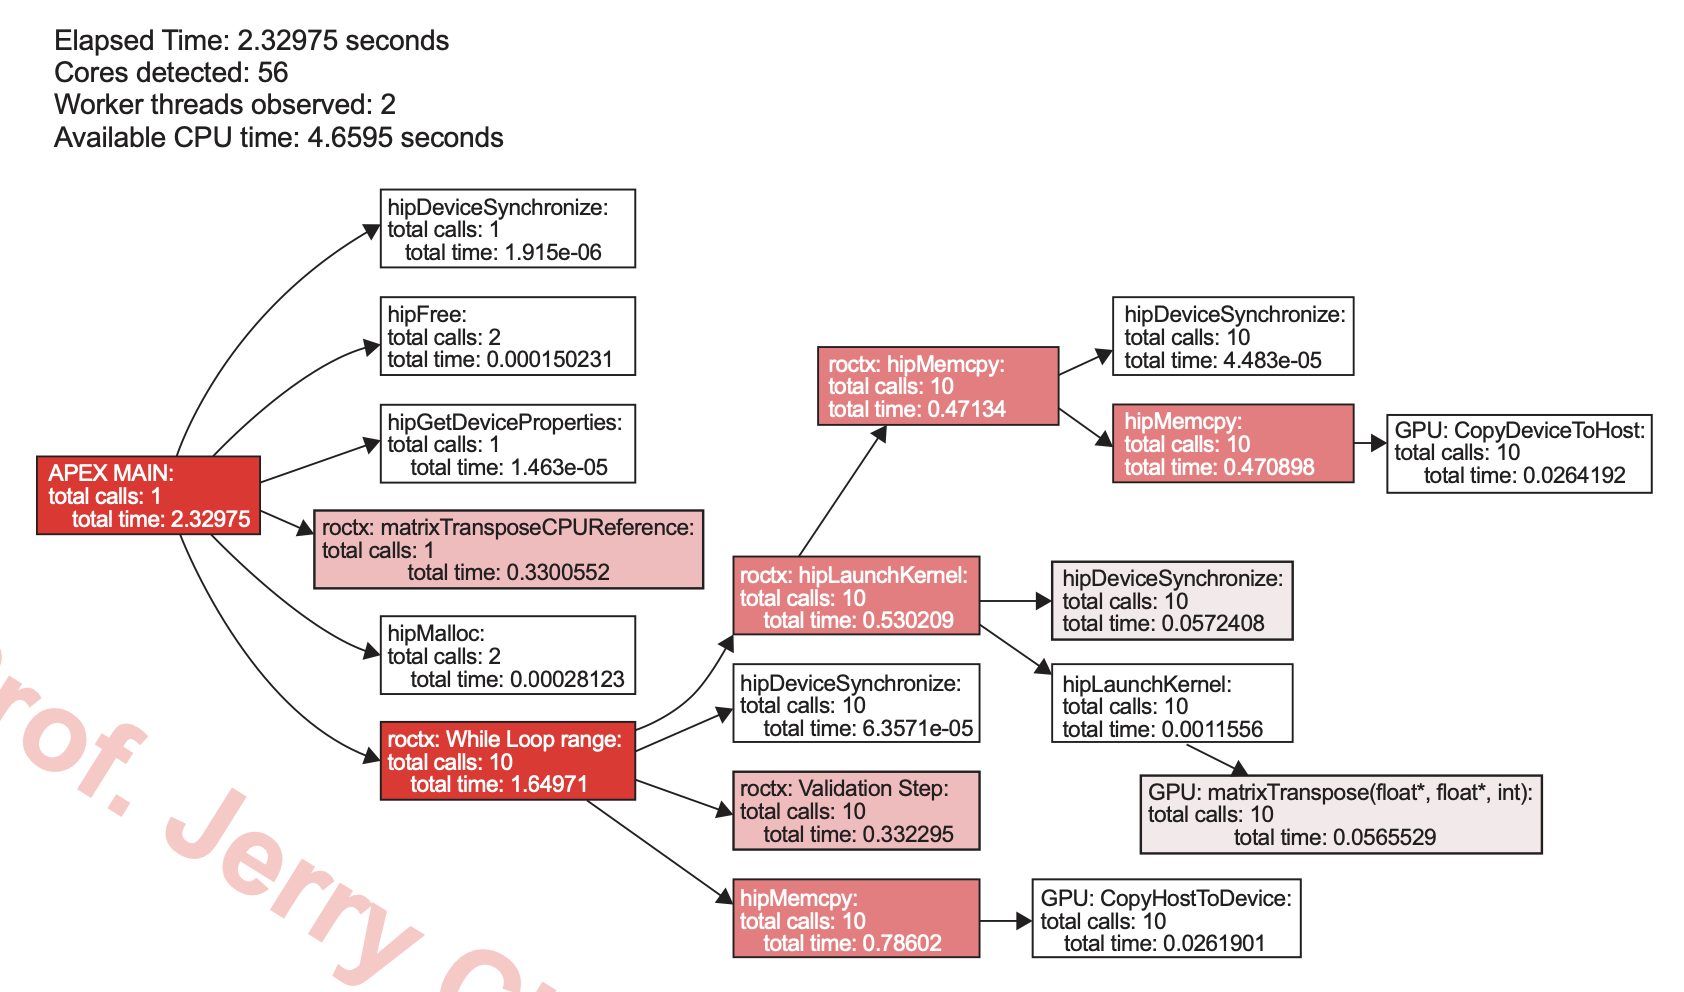
\includegraphics[width=0.9\linewidth]{FileAusiliari/Screenshots/Figure13-21.png}
    \caption{APEX 任務依賴樹由 Graphviz 渲染。紅色表示任務圖中每個節點的相對耗時。需要注意的是,由於某些樹節點在多個執行緒或device上同時執行,其累積時間可能超過總執行時間。HIP API 調用和device活動被捕捉到依賴樹中,且 APEX 還捕捉了 ROCTX 插桿調用與標記。}
    \label{fig:PAPI21}
\end{figure}

APEX 提供了一個類似 tauexec 的剖析工具,名為 apexexec,該工具會自動預載入 APEX 測量庫並設置適當的環境變數來剖析支援的執行時環境。例如,要執行一個 HIP 範例程式(如 Matrix-Transpose\_hip),用戶在程式前添加 apexexec,並將任何與 APEX 相關的參數添加為 --apex 前綴。

在此範例中,啟用了多個選項,使其更具趣味性:

該程式對一個 8,192 × 8,192 的矩陣進行 10 次轉置操作,每次結果都與參考的 CPU 執行進行比較。為了增加趣味性,CPU 執行和驗證使用了 OpenMP 並行處理。APEX 使用 rocTracer 庫測量 HIP CPU 和 GPU 活動,並定期使用 rocProfiler 和 ROCm SMI [22] 捕捉 GPU 狀態計數器,採樣週期設置為 10,000 μs(100 Hz)。數據被寫入 JSON 追蹤事件檔 [33],以供 Perfetto [32] 進行可視化,同時任務樹被寫入機器與人類可讀的文字檔。

hipcc 編譯器和執行時還支援 OpenMP 剖析介面(OMPT),因此啟用了與 OMPT 相關的選項。圖 13.21 顯示了使用 Graphviz [14] 的 dot 工具渲染的任務樹。為了使圖表更易讀,此次執行未啟用 OMPT 支援。

圖 13.20 中,追蹤檔通過 Perfetto 渲染,定期捕捉了多個host和device端的度量指標,包括功耗和溫度、記憶體使用率、GPU 和 GPU 記憶體利用率等。stream事件通過 CPU 執行緒 0 與 HIP 活動之間的紅色箭頭進行可視化,揭示了資源間的控制stream依賴關係。APEX 還捕捉了使用 ROCTX API 添加的 CPU 插桿範圍與標記,該 API 由 ROC-Tracer 庫提供。


\subsection{TAU 總結}

\begin{figure}
    \centering
    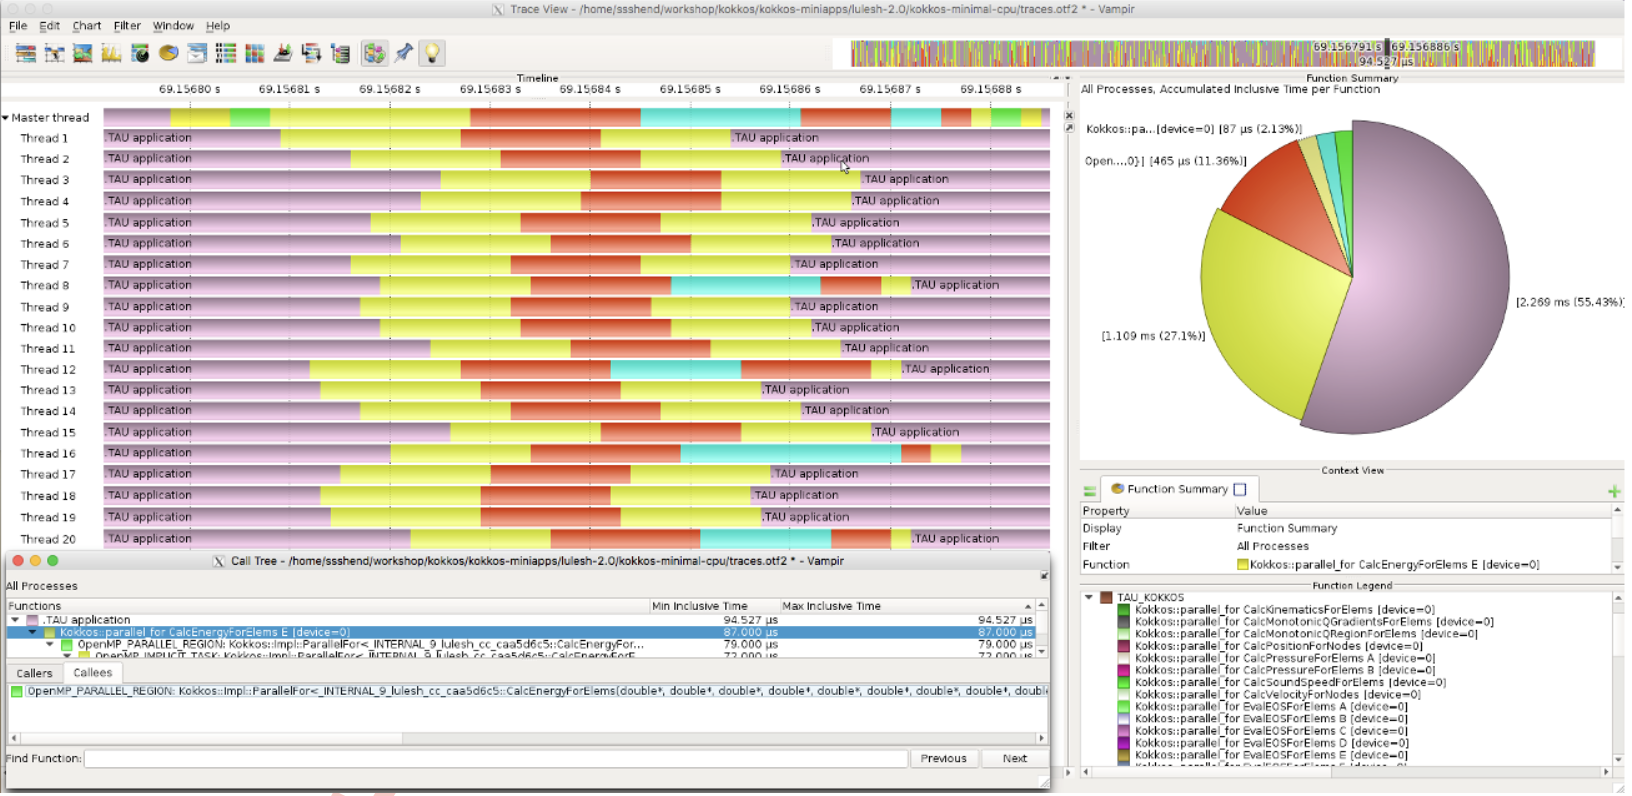
\includegraphics[width=0.9\linewidth]{FileAusiliari/Screenshots/Figure13-22.png}
    \caption{TAU 的 OTF2 追蹤資料使用 Vampir 商業追蹤視覺化工具進行視覺化。}
    \label{fig:PAPI22}
\end{figure}

TAU 擁有廣泛的功能,提供了對低階 CPU 和 GPU kernel事件性能的全貌,涵蓋host與device之間以及跨網路的數據傳輸,並支援 OpenMP、OpenACC、OpenCL、MPI 和 Kokkos。對於非同步執行的支援體現在 TAU 的 APEX 測量層中,而對剖析和追蹤的可視化、數據捕捉與存儲性能的支援則由其 TAUdb 資料庫系統提供。對於跨實驗分析與數據挖掘,TAU 的 perfexplorer [35] 支援擴展性能工程,提供了強大的分析工具。

\section{TotalView Debugger}


\begin{figure}
    \centering
    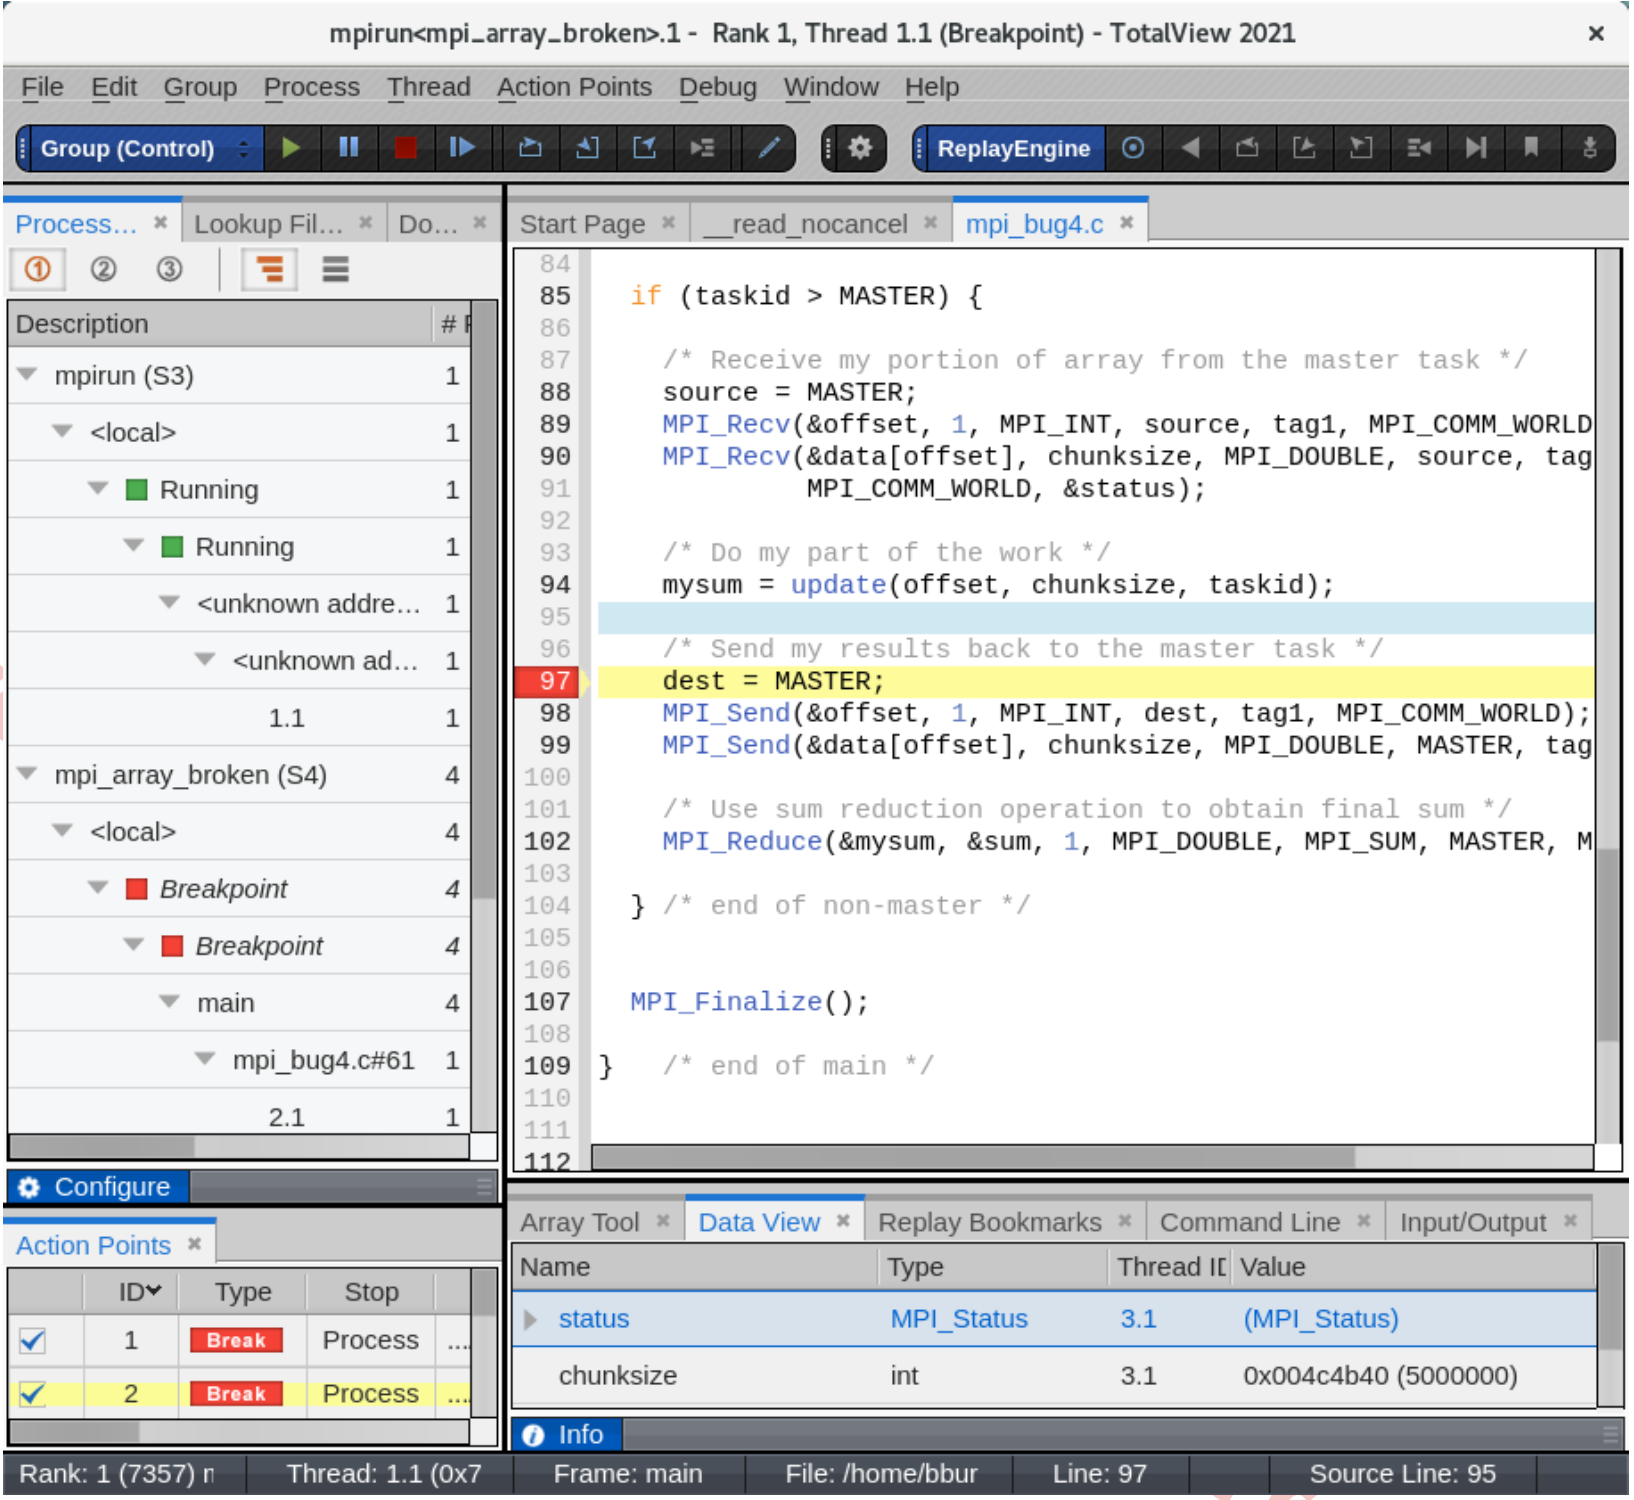
\includegraphics[width=0.9\linewidth]{FileAusiliari/Screenshots/Figure13-23.png}
    \caption{使用 TotalView 進行平行除錯}
    \label{fig:PAPI23}
\end{figure}

TotalView for the HPC Debugger 是由 Perforce Software 開發的除錯工具,擁有超過 30 年的發展歷史。在此期間,它通過為 AMD、Cray、HP、IBM、Intel、SGI、Sun 等硬體廠商提供除錯器,持續支持 HPC 社群。TotalView 可在 Unix、Linux、macOS 和自定義kernel上運行,並隨著 HPC 領域的持續變化,不斷適應新的架構、語言和技術。

如今,TotalView 是一個功能豐富的除錯器,支持 C、C++ 和 Fortran 程式語言,包含使用這些語言和 Python 建構的多語言應用程式。它還支援多種混合的平行程式設計範式,例如 MPI、OpenMP、pthreads、HIP、CUDA、Open Accelerators (OpenACC)、Unified Parallel C、Coarray Fortran、Global Arrays 和 Symmetric Hierarchical Memory。

TotalView 提供了一個易於使用的圖形使用者介面(GUI)(見 圖 13.23)和命令列介面(CLI)進行互動式除錯。程式設計師可以通過一個單一的控制中心,對多語言和平行程式設計範式組成的多進程和多執行緒進行除錯。標準的除錯功能包括啟動和停止執行緒、進程及群組。支持源碼級和指令級的單步執行與跳過執行,並提供斷點和條件斷點功能。可以顯示源碼、變數、陣列、記憶體塊和暫存器,並允許修改程式狀態。

CLI 是一個可程式化的工具命令語言解釋器,支持創建用戶自定義工具來擴展除錯器的功能,並提供了一種腳本語言,用於實現自動化操作。TotalView 可以通過其 TVScript 和 MemScript 框架以腳本模式運行,支持非互動式的批處理除錯。該框架基於事件-行為模型,允許程式設計師定義程式中可能發生的事件以及事件發生時需要執行的行為。數據會記錄到一組輸出檔案中,供批處理任務完成後進行審查。


TotalView 提供多種其他除錯功能,包括 C、C++ 和 Fortran 表達式求值器、數據監視點、C++ 標準模板庫元素可視化器(如 map、set、array、list、string 等)、進程與執行緒顯示聚合器、記憶體除錯器、kernel檔除錯器、非同步執行緒控制器、反向除錯器、異構除錯器,以及內建的幫助和文檔工具。

這些功能使程式設計師能夠理解其複雜應用程式的運行方式並識別潛在的邏輯錯誤。除了發現軟體缺陷,TotalView 還能幫助理解新程式碼,其動態分析功能讓程式設計師能夠以可視化數據的方式體驗程式的運行過程。

TotalView 的需求包括:
支援 X11 的 GUI 客戶端。
功能全面的進程與執行緒追蹤介面(如 ptrace 或 /proc 文件系統)。
生成準確除錯資訊的編譯器(如 可執行與可連結格式 (ELF)、DWARF 或 符號表字符串)。MPI-and-Rationals 介面。libpthread\_db 執行緒級追蹤介面。支援多節點除錯的 TCP/IP 套接字和遠程 Shell(如 SSH)。AMD GPU Debug API 和 NVIDIA CUDA Debug API。
TotalView 提供對 AMD 和 NVIDIA GPU 的先進除錯支援。程式設計師可以在同一會話中輕鬆除錯多個節點上的多個 GPU。利用 TotalView 的 GPU 功能,程式設計師可以輕鬆理解程式碼的運行方式,逐行檢查程式碼、檢視 GPU 特定數據,並對 CPU 和 GPU 程式碼進行除錯。TotalView 支援多種針對 GPU 的常見語言,包括 CUDA、HIP、OpenCL 和 OpenMP。

TotalView 支援異構應用程式的除錯,這些應用程式涉及多種處理器架構的組合(如 PowerPC、x86\_64 和各種 GPU)。TotalView 的位址空間模型支援包含多個異構位址空間的進程,其中不同的執行緒可以在其 GPU device上下文中運行,或者與其他執行緒共享進程位址空間(如 pthreads)。隨著程式設計語言擴展以支持加速device(如 OpenMP target 構造),位址空間模型允許 TotalView 更準確地重建進程作為 CPU 或 GPU 容器的概念模型。



TotalView 為執行於 AMD GPU 上的 HIP 應用程式提供了全面的除錯支援。對於 HIP 或任何 AMD GPU 應用程式的除錯方式與其他類型應用程式類似。大多數適用於 CPU 的指令和操作也適用於 GPU。程式設計師可以執行以下操作:

\begin{itemize}
    \item 啟動、附加到進程或從進程分離,包括 MPI 進程。
    \item 顯示 SGPR、VGPR、通用暫存器和特殊暫存器。
    \item 顯示反組譯的機器指令。
    \item 創建、刪除、啟用和停用斷點。
    \item 通過單步執行追蹤源碼和指令級代碼。
    \item 回溯堆疊。
    \item 顯示變數(受限於編譯器生成的除錯資訊)。
\end{itemize}

HIP 應用程式應使用 -ggdb 和 -O0 除錯選項進行編譯。通過與 -Wl,-R/opt/rocm/hip/ 選項連結,應用程式可以自動找到 HIP 共享庫。

\begin{lstlisting}[caption={Listing 13.1: Example compiling a \textit{HIP} program for \textit{TotalView}.}]
hipcc -O0 -ggdb -c bit_extract.cpp -o bit_extract.o
hipcc -Wl,-R/opt/rocm/hip/ bit_extract.o -o bit_extract
\end{lstlisting}

除錯會話可以通過在 TotalView 下運行目標應用程式或附加到已運行的程式來啟動。使用 TotalView -rocm 選項可確保啟用 AMD GPU 的除錯功能。

\begin{lstlisting}[caption={Listing 13.2: Example HIP debugger launch in TotalView.}]
totalview -rocm -args bit_extract
\end{lstlisting}

TotalView 提供了統一的視圖,展示所有影像檔案(如可執行檔、共享庫和 GPU ELF 映像)及所有源碼檔案中的源碼和行級斷點。因此,任何在運行時動態加載的程式碼(包括 AMD GPU ELF 映像)都會在源碼顯示中統一呈現。在源碼行上設置斷點後,無論該源碼的機器碼是否已加載,當執行到該行時,程式會在該行或附近停止。程式設計師可以在動態加載的程式碼(如共享庫和 GPU 映像檔案)中設置待處理的斷點。要設置待處理的斷點,只需在源碼顯示中選擇行號,TotalView 會安排程式盡可能靠近該源碼行停止。

預設情況下,HIP 運行時會推遲 GPU 程式碼的加載,直到首次啟動kernel。因此,在 HIP 源碼中添加的所有斷點必須事先設置為待處理斷點。然而,將 HIP\_ENABLE\_DEFERRED\_LOADING(HIP 的環境變數)設置為零,可以禁用推遲的 GPU 程式碼加載。這樣可以確保 GPU 程式碼在應用程式進入主函式前已加載。當禁用 GPU 程式碼的推遲加載後,在進入主函式時,GPU 源碼行資訊將變得可用,無需等待首次kernel啟動,從而更容易在 GPU 程式碼中設置源碼級斷點。

TotalView 為進程中的每個 GPU 代理(device)分配一個負的調試執行緒 ID(DTID)。例如,使用兩個 GPU device的進程將有兩個調試 GPU 代理執行緒(例如,-1 和 -2)。程式設計師可以通過選擇進程內的 GPU 代理執行緒來專注於特定device。

TotalView 為 Linux CPU 進程位址空間和每個 GPU 代理執行緒的位址空間分別維護獨立的位址空間。這些位址空間被放置在同一個 TotalView 共享組中,該共享組包含程式創建並共享的所有進程。

斷點在共享組中創建並進行評估,並應用於共享組中的所有影像檔案(例如,可執行檔案、共享庫和 GPU ELF 映像)。因此,斷點既可以應用於 CPU 程式碼,也可以應用於 GPU 程式碼。這允許在host程式碼中的源碼行上設置斷點,當 GPU 程式碼加載後,斷點會在 GPU 映像中的相同位置被設置。

\begin{figure}
    \centering
    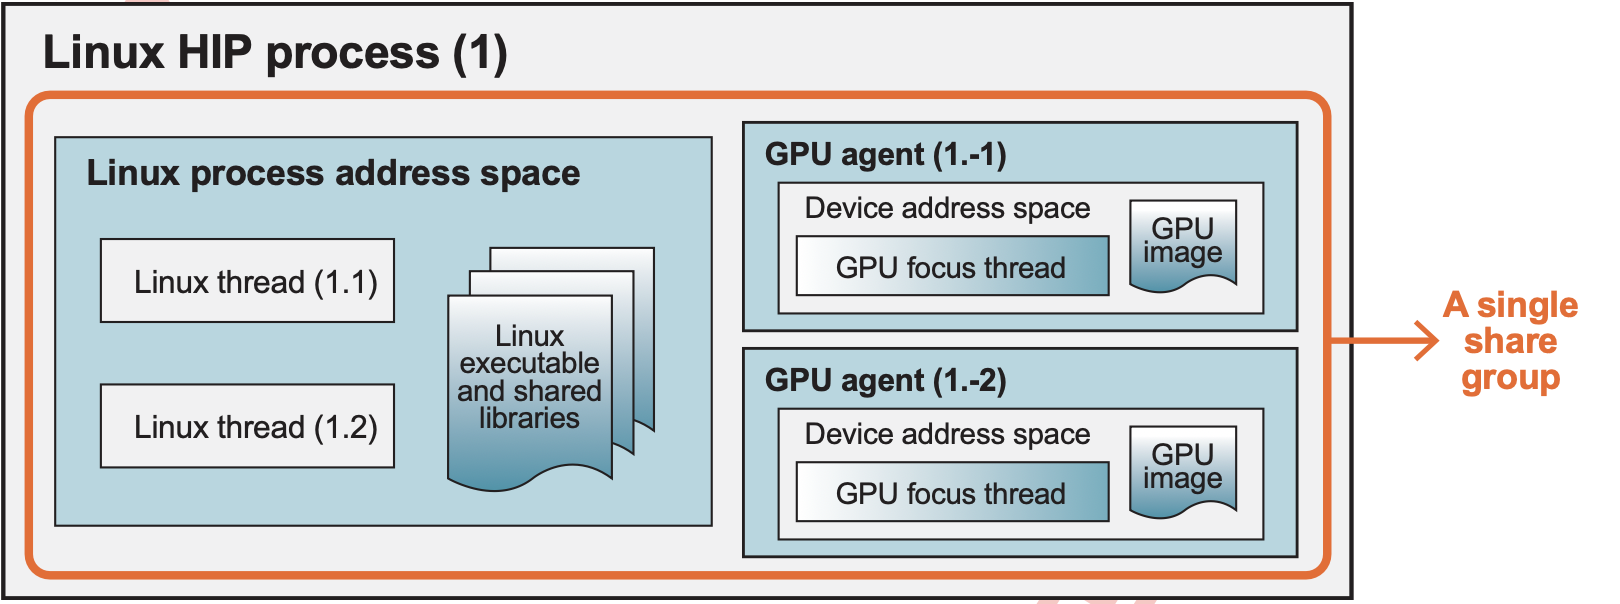
\includegraphics[width=0.9\linewidth]{FileAusiliari/Screenshots/Figure13-24.png}
    \caption{TotalView 的 HIP 除錯模型。}
    \label{fig:PAPI24}
\end{figure}


如果我們有一個包含兩個 pthread 和兩個 GPU 代理執行緒的 Linux 進程,則 GPU 除錯模型可總結如下:

Linux 進程位址空間,包含一個 Linux 可執行檔案和一個 Linux 共享庫列表。
一組 Linux 執行緒:
被分配一個正的 DTID。
與其他 Linux 執行緒共享 Linux 進程位址空間。
與一組 GPU 代理執行緒共享:
被分配一個負的 DTID。
擁有與 Linux 進程位址空間分離且與其他 GPU 代理執行緒分離的位址空間。
擁有一個 GPU 焦點執行緒,專注於 GPU 代理執行緒內的特定硬體通道。
上述 TotalView HIP 除錯模型在 TotalView GUI 和 CLI 中得以反映。此外,ROCm 特定 CLI 指令允許程式設計師檢視 GPU 代理執行緒,將焦點切換到特定通道,並顯示 GPU 代理、隊列、派遣、工作組、波前和工作項的狀態。


\section{HPCToolkit}

Rice University 的 HPCToolkit 性能工具支持通過記錄 CPU 和 GPU 活動的調用路徑剖析和追蹤來測量和分析 GPU 加速應用程式 [83]。為了幫助程式設計師理解應用程式如何使用 GPU 操作,HPCToolkit 提供了針對每個 GPU 操作的度量,並屬性化該操作在其調用上下文中的貢獻。為補充記錄的 GPU 操作的時間和語義資訊,HPCToolkit 還使用硬體性能計數器來測量 GPU 操作。

HPCToolkit 支援多種 CPU 架構(如 x86-64、Power 和 ARM)、不同供應商的 GPU(如 AMD、Intel 和 NVIDIA),以及各種將計算卸載到 GPU 的程式設計模型(如 CUDA [56]、HIP [4]、Raja Portability Suite [15]、Kokkos [26]、OpenMP [60] 和 Data Parallel C++ [37])。

接下來,我們將描述 HPCToolkit 的工作流程,並提供兩個範例,演示其如何分析由 AMD GPU 加速的應用程式的性能。


\subsection{HPCToolkit流程}

\begin{figure}
    \centering
    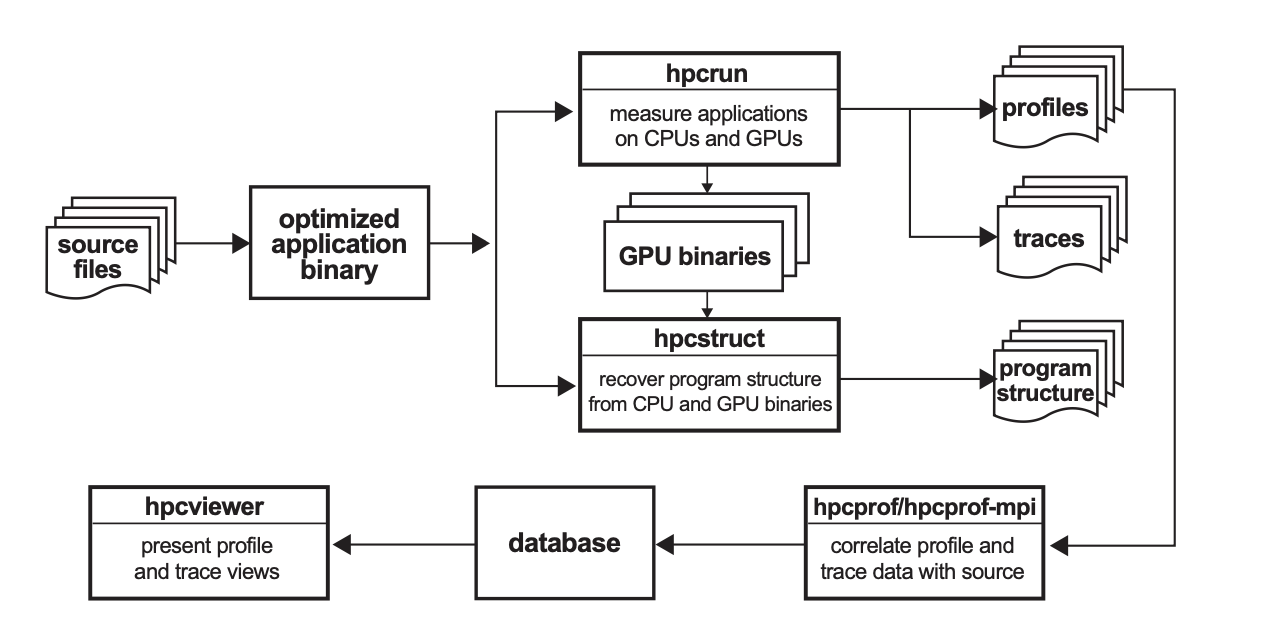
\includegraphics[width=0.9\linewidth]{FileAusiliari/Screenshots/Figure13-25.png}
    \caption{HPCToolkit 用於分析 GPU 加速應用程式的工作流程。}
    \label{fig:PAPI25}
\end{figure}

圖 13.25 展示了 HPCToolkit 用於分析 GPU 加速應用程式性能的工作流程。HPCToolkit 的 hpcrun 測量工具使用採樣技術測量 CPU 活動,並通過 GPU 廠商提供的剖析 API 收集 GPU 性能指標。hpcrun 可測量使用一種或多種 GPU 程式設計模型的程式。

在程式執行期間加載 GPU 二進位檔時,hpcrun 記錄它們以便後續分析。對於提供細粒度測量 API 的 GPU,hpcrun 使用硬體支援或二進位插桿收集 GPU kernel的指令級特徵。

hpcrun 的輸出包括 CPU 和 GPU 活動的剖析檔和可選的追蹤檔。每個剖析檔包含一個 調用上下文樹,其中每條調用路徑(由樹節點表示)與一組指標(如執行時間和執行的指令數)相關聯。每個追蹤檔則包含 CPU 執行緒或 GPU stream的調用路徑和時間戳對的序列。


hpcstruct 分析 CPU 和 GPU 二進位檔以恢復有關程序、內聯函式、迴圈嵌套和源碼行的靜態資訊。此過程有兩個重要方面:從二進位檔中恢復行映射和內聯編譯器記錄的資訊,以及分析機器碼以恢復迴圈相關資訊。

hpcprof 和 hpcprof-mpi 使用 hpcstruct 生成的資訊,將 GPU 加速程式執行期間收集的性能指標與源碼上下文相關聯。hpcprof 使用單個節點聚合剖析和追蹤,將與機器指令相關的測量結果映射回 CPU 和 GPU 源碼。hpcprof-mpi 則利用分散式記憶體並行技術,加速對極大規模執行的性能分析。

最後,hpcviewer 解釋並可視化由 hpcprof 和 hpcprof-mpi 生成的資料庫。在剖析視圖中,hpcviewer 展示跨越 CPU 和 GPU 上下文的異構調用上下文樹,並附有測量或推導的指標,以幫助使用者評估程式碼性能並識別瓶頸。在追蹤視圖中,hpcviewer 以時間軸的形式展示 CPU 和 GPU 活動,幫助程式設計師理解應用程式執行過程中的時間變化行為。

\subsection{用HPCToolkit分析PIConGPU}
PIConGPU [16] 是一個完全相對論性、多核、3D3V 的粒子模擬(Particle-in-Cell, PIC)程式碼。在下一節中,我們將展示如何使用 HPCToolkit 測量 PIConGPU 在 16 個 MPI ranks 和 16 個 MI100 GPUs 上運行的性能。


\subsection{收集並分析profiles和traces}
第一步,使用 hpcrun 測量 PIConGPU 的性能,如 Listing 13.3 所示。
\begin{lstlisting}[caption={Listing 13.3: Example of the hpcrun command.}]
hpcrun -t -e REALTIME -e gpu=amd -o picgongpu.m picongpu
\end{lstlisting}

在上述命令中:

-t 指示 hpcrun 收集追蹤數據。
-e REALTIME 表示 hpcrun 應以相等的實時間隔對每個 CPU 執行緒進行採樣,即使執行緒處於空閒狀態也會記錄樣本。
-e gpu=amd 指定使用 AMD ROCm 支援收集 GPU 剖析數據。
-o picongpu.m 指示 hpcrun 將測量數據存儲在 picongpu.m 目錄中。
第二步,使用 hpcstruct 恢復程式結構,如 Listing 13.4 所示。

\begin{lstlisting}[caption={Listing 13.4: Example of the hpcstruct command.}]
hpcstruct picgongpu.m
\end{lstlisting}

預設情況下,hpcstruct 使用當前節點上一半的硬體執行緒來對應用程式的可執行檔、共享庫和 GPU 二進位檔進行並行分析,以恢復其程式結構。通過檢查由 hpcrun 記錄的 picongpu.m 測量目錄的內容,hpcstruct 確定應分析的 GPU 和 GPU 二進位檔,並將結果添加到測量目錄中。

第三步,使用 hpcprof,結合 hpcstruct 恢復的程式結構資訊解釋性能測量數據,如 Listing 13.5 所示。

\begin{lstlisting}[caption={Listing 13.5: Example of the hpcprof command.}]
hpcprof -o picgongpu.d picgongpu.m
\end{lstlisting}

-o 選項指定了 hpcprof 將其分析結果寫入的輸出目錄名稱。
最後一步,使用 hpcviewer 檢視由 HPCToolkit 收集的剖析和追蹤數據,如 Listing 13.6 所示。

\begin{lstlisting}[caption={Listing 13.6: Example of the hpcviewer command.}]
hpcprof -o picgongpu.d picgongpu.m
\end{lstlisting}

\begin{figure}
    \centering
    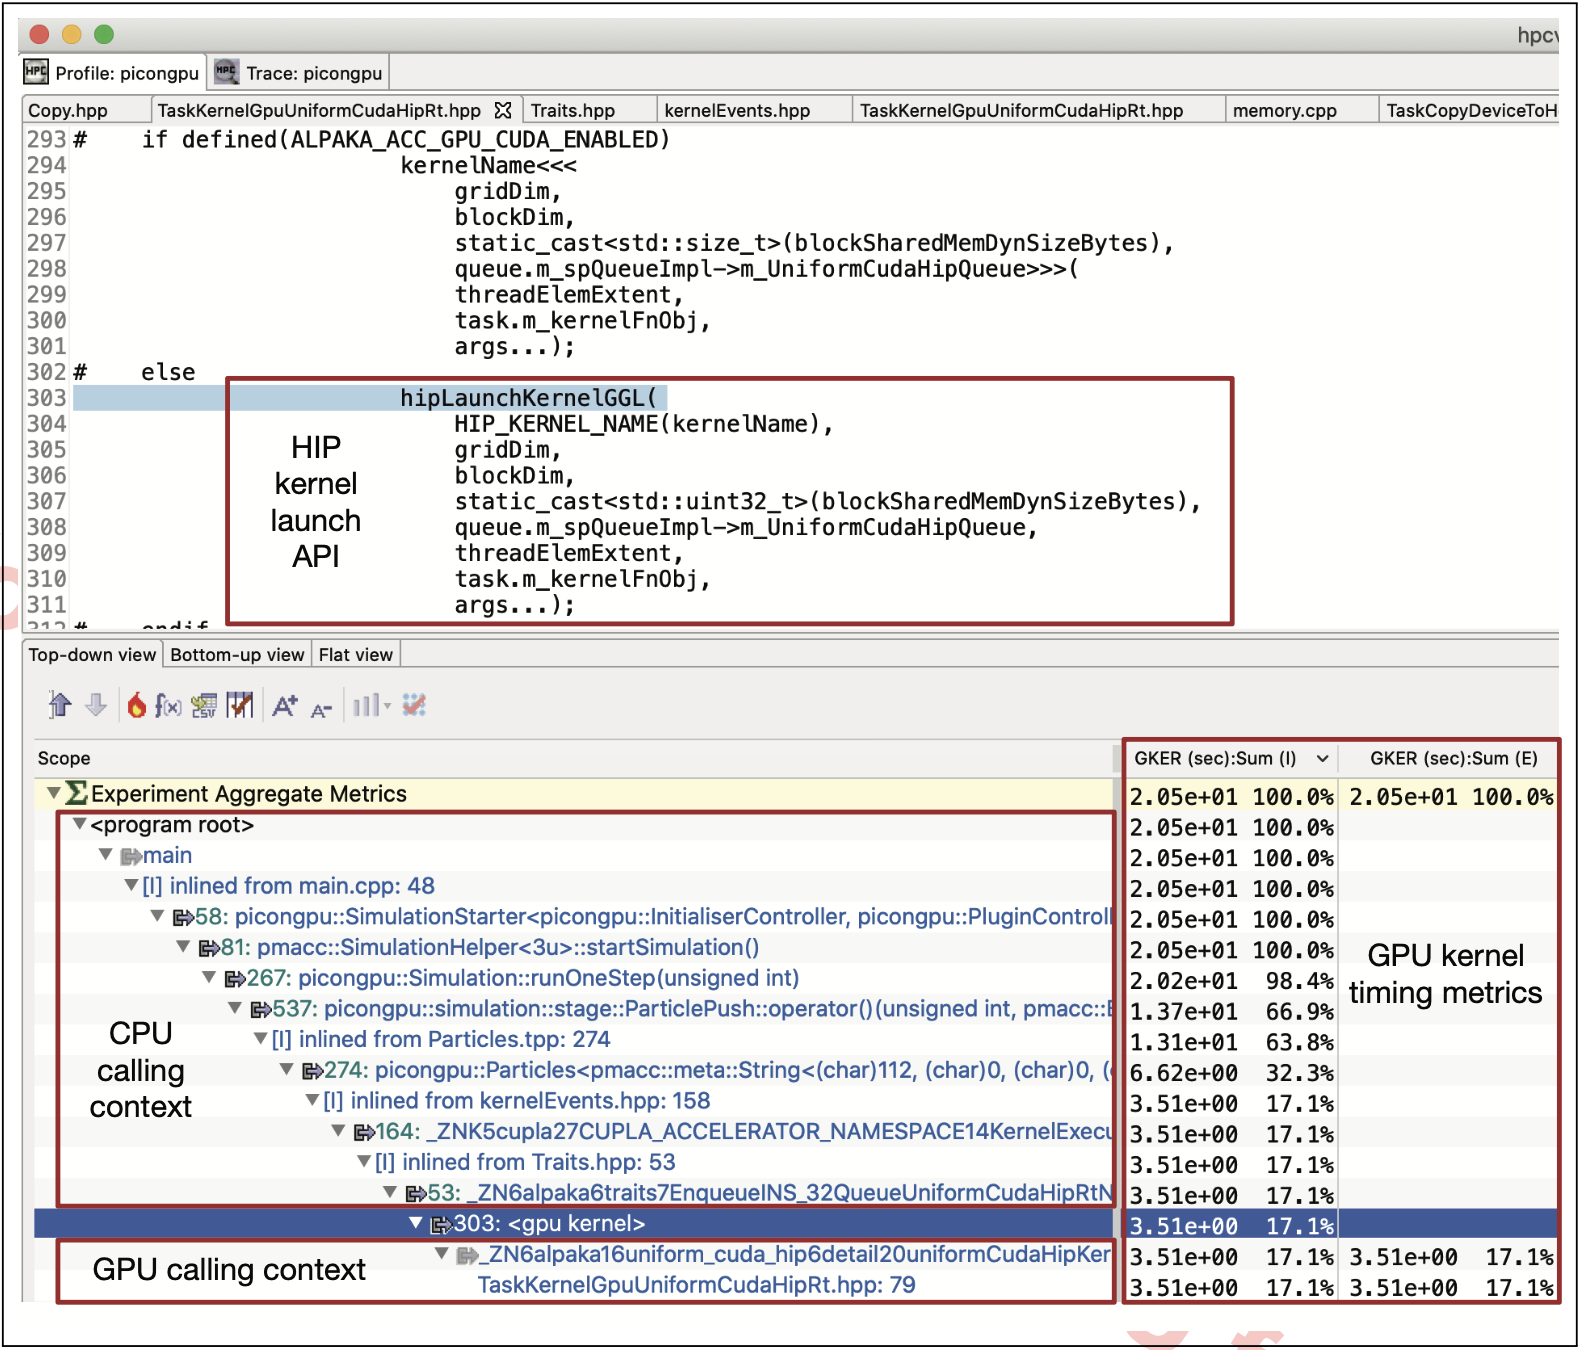
\includegraphics[width=0.9\linewidth]{FileAusiliari/Screenshots/Figure13-26.png}
    \caption{PIConGPU 的由上而下的剖面圖。}
    \label{fig:PAPI26}
\end{figure}

圖 13.26 展示了 PIConGPU 中一個熱點kernel的自上而下剖析視圖。左下方的 scope pane 顯示了其統一的 CPU–GPU 調用上下文,包含三個部分:啟動kernel的 HIP API 的 CPU 調用上下文、表示從host到device過渡的佔位框架(即 <gpu kernel>),以及 GPU 調用上下文。目前,在 AMD GPU 上的 GPU 調用上下文僅包含 GPU kernel,因為目前不支援kernel內的細粒度測量。

圖 13.26 展示了 GPU kernel執行時間,右下方的面板顯示了一系列性能指標的列。HPCToolkit 還可以顯示進出 GPU 記憶體的拷貝操作的指標。頂部的 source pane 顯示了 HIP API(如 hipLaunchKernelGGL)的源碼行。用戶只需點擊調用上下文中的函數,即可導航到該函數的源碼位置。


\begin{figure}
    \centering
    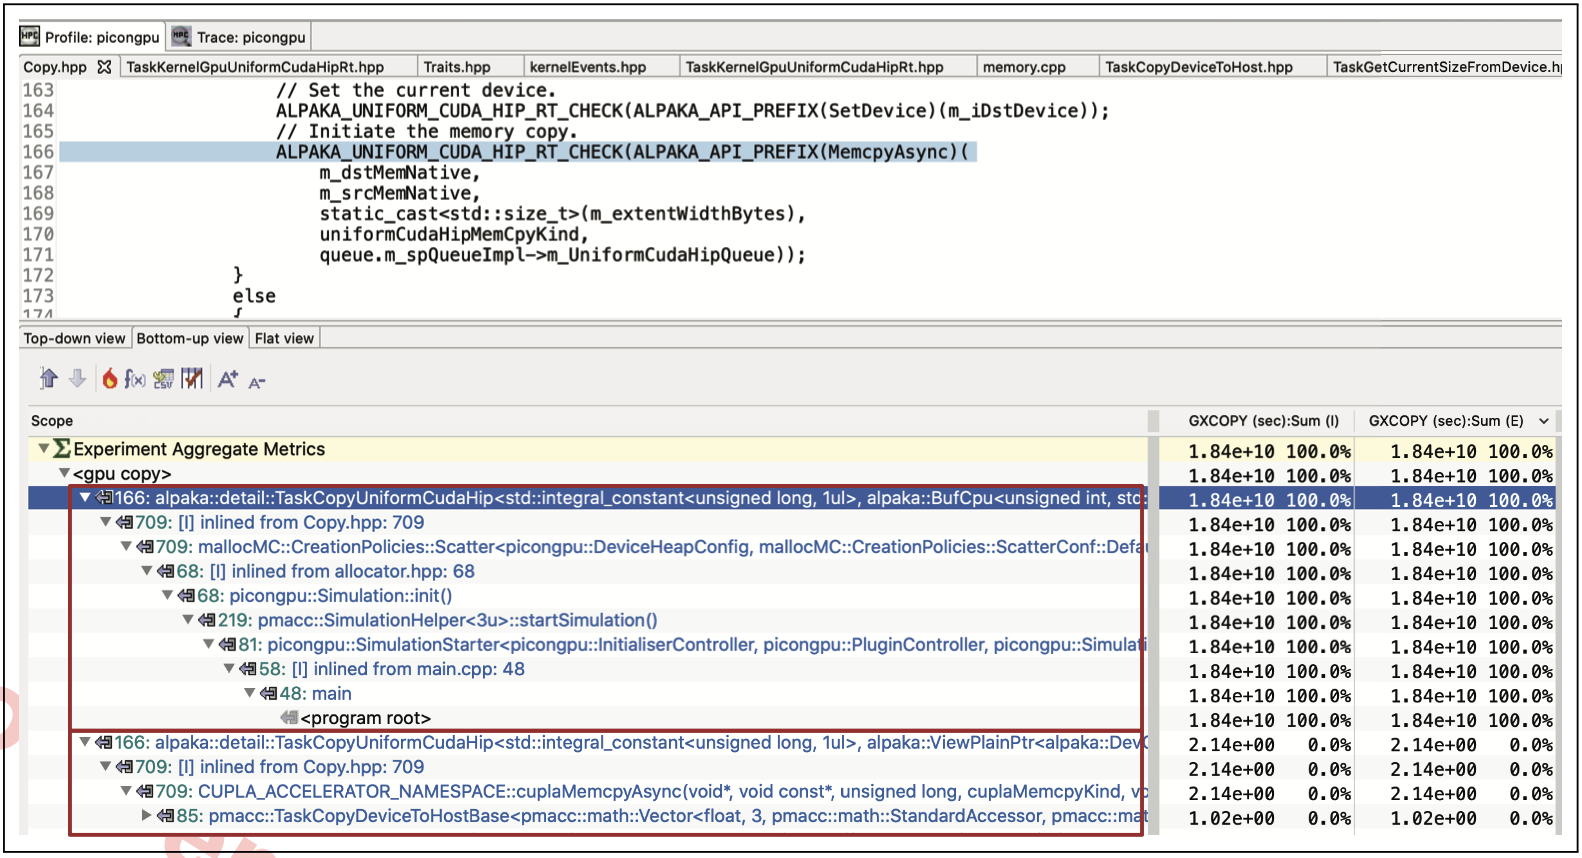
\includegraphics[width=0.9\linewidth]{FileAusiliari/Screenshots/Figure13-27.png}
    \caption{PIConGPU 的由下而上的剖面圖。}
    \label{fig:PAPI27}
\end{figure}
圖 13.27 展示了 GPU 記憶體拷貝操作的自下而上剖析視圖。scope pane 中函數的自下而上調用上下文顯示了該函數被調用的一個或多個上下文。

在圖中,由佔位框架 <gpu copy> 表示的 GPU 記憶體拷貝操作在兩個不同的調用上下文中被調用,這兩個上下文分別對應於不同模板的實例化。在這個例子中,頂部上下文幾乎負責了所有的 GPU 拷貝成本。

在這種情況下,我們只需要檢查頂部調用路徑即可了解大部分 GPU 拷貝操作的成本來源。通常,一個操作的成本會根據多個調用上下文更均勻地分佈。自下而上的視圖通過將操作的所有調用上下文分組,使得理解這一點變得更加簡單。

\begin{figure}
    \centering
    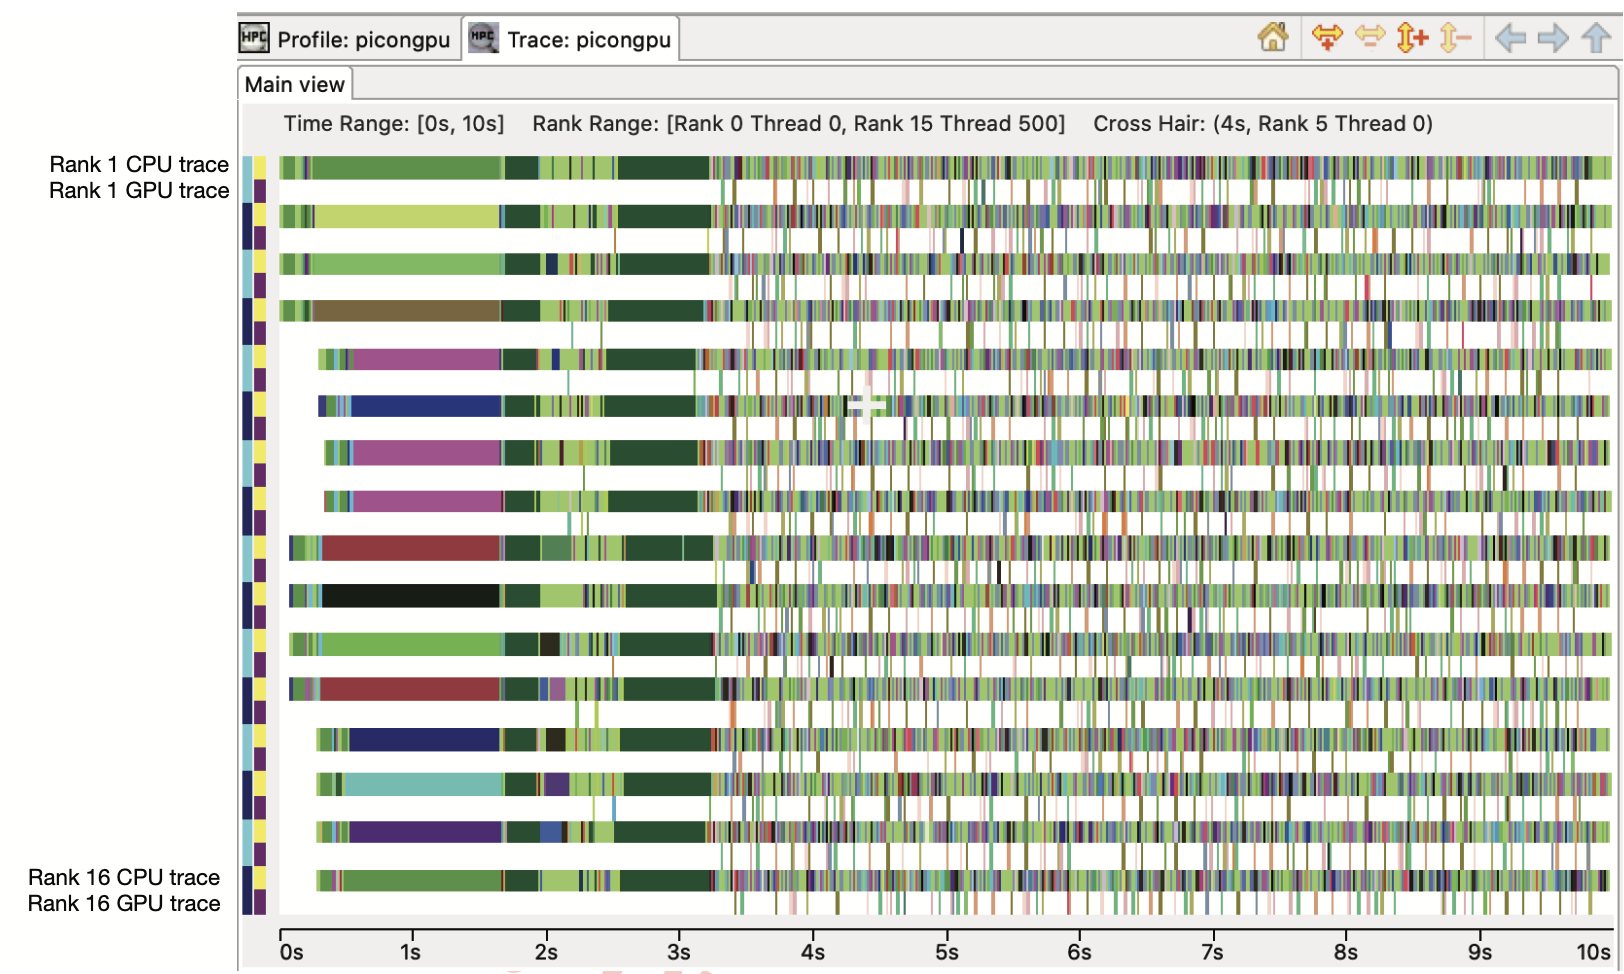
\includegraphics[width=0.9\linewidth]{FileAusiliari/Screenshots/Figure13-28.png}
    \caption{Trace view.}
    \label{fig:PAPI28}
\end{figure}

圖 13.28 展示了一個統一的 CPU–GPU 追蹤視圖。追蹤線從上到下分別表示 MPI ranks 1–16 的 CPU 執行緒和 GPU stream。每個 MPI rank 的執行也使用了一個 MPI 輔助執行緒,我們通過 hpcviewer 的 Filter 選單在追蹤視圖中隱藏了這些執行緒,因為它們在執行期間始終處於空閒狀態。

從追蹤視圖中可以看到,在執行的前三分之一期間,GPU 追蹤線為白色,表示 GPU 處於空閒狀態。這段時間代表應用程式的初始化階段。在剩餘的執行期間,每條 GPU 追蹤線上出現了零散的操作,表明 GPU 並未被完全利用。因此,程式設計師應仔細檢查 CPU 執行緒,以了解在 GPU 處於空閒狀態時它們正在執行的操作。



\subsection{使用硬體計數器進行測量}

HPCToolkit 使用田納西大學的 PAPI [71] 工具包(如本章前面所述)通過硬體計數器測量 GPU 活動。目前,工具將硬體計數器測量與單個 GPU kernel相關聯的唯一方法是使用現有供應商的 API 將kernel進行序列化,並在每次執行前後讀取計數器數據。然而,序列化kernel會減慢執行速度,並可能改變程式的行為。

我們使用 FloydWarshall,一個 HIP 範例程式 [7],來展示 HPCToolkit 利用 GPU 硬體計數器測量應用程式性能特徵的能力。以下命令指示 HPCToolkit 使用 PAPI 測量 AMD GPU TCC(共享 L2 快取) 的命中和未命中情況。該命令如 Listing 13.7 所示。

\begin{lstlisting}[caption={Listing 13.7: Command for collecting the TCC miss counter for the FloydWarshall application using HPCToolkit.}]
hpcrun -e gpu=amd -e rocm:::TCC_HIT_sum:device=0  -e rocm:::TCC_MISS_sum:
    device=0 .∕FloydWarshall -q -i 100
\end{lstlisting}

如前所述,我們使用 hpcstruct 和 hpcprof 分析生成的測量資料庫。

圖 13.29 展示了與 GPU 調用上下文相關聯的硬體計數器指標的資料庫。利用 hpcviewer 的指標過濾功能,我們隱藏了帶有獨占命中和未命中指標的列,並計算 TCC 未命中率為 100 × misses/(hits + misses)。

圖 13.29 顯示,對於 FloydWarshallPass kernel,TCC 未命中率僅為 6.87\%,但對於 Line 356 的一對 hipHostMalloc 操作,未命中率達到了 100\%。這些資訊對於識別 GPU 程式碼上下文中記憶體層次結構利用率較差的部分非常有用。

\begin{figure}
    \centering
    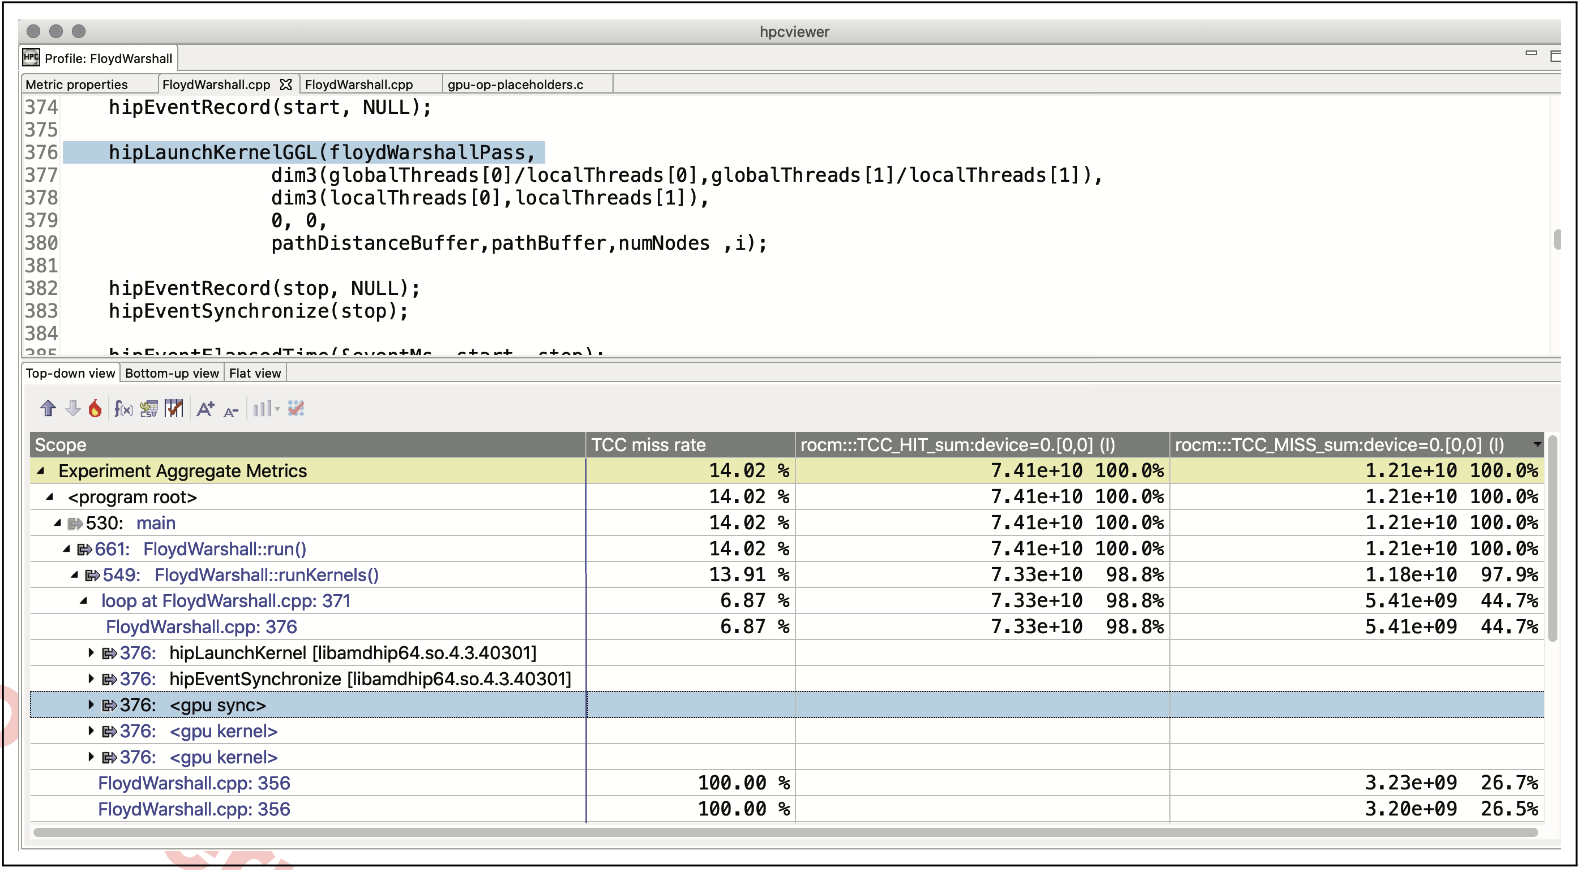
\includegraphics[width=0.9\linewidth]{FileAusiliari/Screenshots/Figure13-29.png}
    \caption{將硬體計數器指標與其呼叫上下文中的 GPU 操作關聯起來。}
    \label{fig:PAPI29}
\end{figure}

\section{用Linaro Forge來做debugging和profiling}

Linaro Forge 結合了 Linaro DDT(用於平行高性能應用程式除錯)、Linaro MAP(用於性能剖析與優化建議)以及 Linaro Performance Reports(用於總結和表徵標量與 MPI 應用程式性能)。Linaro Forge 支援多種平行架構與模型,包括 MPI、CUDA 和 OpenMP。它是一個跨平台工具,支援最新的編譯器與 C++ 標準,以及 Intel、64-bit Arm、AMD、NVIDIA GPU 和 AMD GPU 硬體。

Linaro Forge 提供了除錯、修復和剖析程式所需的一切,適用於任何規模的應用程式。一個統一的介面讓程式設計師在程式碼開發過程中輕鬆切換 Linaro DDT 與 Linaro MAP。Linaro Forge 提供了原生的遠程客戶端,適用於 Windows、Mac OS X 和 Linux。通過遠程客戶端連接到您的叢集,您可以進行除錯、剖析、編輯和編譯應用程式檔案。

若要下載 Linaro Forge,請參閱:
https://www.linaroforge.com/downloadForge/

有關 Linaro Forge 的更多資訊,請參閱:
https://docs.linaroforge.com/latest/html/forge

\subsection{Linaro DDT}

Linaro DDT 是一款功能強大的圖形除錯器,適用於各種開發環境,包括:
\begin{itemize}
    \item 單進程與多執行緒軟體,
    \item OpenMP,
    \item 平行(MPI)軟體,
    \item 異質軟體(例如 GPU 軟體),
    \item 混合程式設計範式的混合代碼(例如 MPI 與 OpenMP、MPI 與 HIP、MPI 與 CUDA),以及
    \item 包括客戶端-伺服器應用程式的多進程軟體。
\end{itemize}

Linaro DDT 幫助您發現並修復單執行緒中的問題,或跨數十萬個進程的問題。Linaro DDT 支援靜態分析以突出潛在的程式碼問題,還整合了記憶體除錯功能,用於對陣列進行邊界檢查(包括讀取和寫入),並與 MPI 消息隊列相結合。

\subsection{Linaro MAP}

Linaro MAP 是一款平行剖析工具,幫助程式設計師識別應用程式中最耗時的程式碼行,並試圖解釋這些程式碼行的高成本原因。Linaro MAP 配置簡單,即使是沒有剖析工具經驗的用戶也能充分利用其功能。Linaro MAP 支援:

\begin{itemize}
    \item MPI、OpenMP、CUDA、ROCm,單執行緒與多執行緒程式,
    \item 小型數據檔案:所有數據都在叢集中聚合,無論程式執行的大小或持續時間如何,僅將數百萬字節寫入磁碟,
    \item 先進的源碼視圖:使用戶能夠跨個別函式分析性能,
    \item 收集剖析數據的互動模式與批處理模式,
    \item 豐富的指標集合,提供有關記憶體使用、浮點運算以及 MPI 在進程間使用的數據,包括:
    \begin{itemize}
        \item 各部分程式碼中使用的向量化指令(包括 AVX 擴展)的百分比,
        \item 記憶體操作所耗費的時間及其在時間與進程間的變化,以識別任何快取瓶頸,
        \item 聚合進程與kernel的可視化摘要,以突出程式碼中的任何不平衡區域,
        \item GPU 指標收集與 GPU kernel檢測。
    \end{itemize}
\end{itemize}

\subsection{Linaro 效能報告}

Linaro Performance Reports 是一款低開銷工具,能生成一頁的文本和 HTML 報告,用於總結和表徵標量與 MPI 應用程式的性能。Linaro Performance Reports 提供了一種最有效的方式來表徵和理解 HPC 應用程式運行的性能。一頁的 HTML 報告能回答每個 HPC 用戶關注的一系列重要問題,包括:


\begin{itemize}
    \item 此應用程式是否已針對其運行的系統進行優化?
    \item 它是否從當前的運行規模中受益?
    \item 是否存在影響性能的 I/O 或網路瓶頸?
    \item 可以進行哪些硬體、軟體或配置更改來改善性能?
\end{itemize}

Linaro Performance Reports 基於 Linaro MAP 自適應採樣技術,該技術可最大限度地減少數據存儲需求和應用程式負載。其主要功能包括:

\begin{itemize}
    \item 能夠透明地運行在已優化的生產就緒代碼上,只需在腳本中添加一條命令,
    \item 即使採樣數千個 MPI 進程,也僅在採樣運行期間引入不到 5\% 的應用程式性能下降。
\end{itemize}


\subsection{Linaro DDT來做GPU debugging}

Linaro DDT 可用於除錯使用 AMD GPU device的程式。運行於 GPU 上的程式碼與host CPU 上的程式碼可同時進行除錯。Linaro DDT 支援 AMD ROCm 軟體堆疊。

要使用 Linaro DDT 除錯 GPU 程式,需要具備啟用了 GPU 支援的授權密鑰。此功能是一個附加選項。如果 DDT 授權中未包含 GPU 支援,則在運行對話框中 GPU 選項將被禁用。

使用 AMD ROCm hipcc 編譯器時,kernel程式必須使用 -g 標誌進行編譯。以下語法可生成除錯器所需的符號資訊,並禁用某些可能妨礙除錯的優化:

\begin{lstlisting}
$ hipcc –g -O0 -o program_name source_file.cpp
\end{lstlisting}

要開始Linaro DDT:
\begin{lstlisting}
$ ddt --rocm <program_name> [arguments]
\end{lstlisting}

\begin{figure}
    \centering
    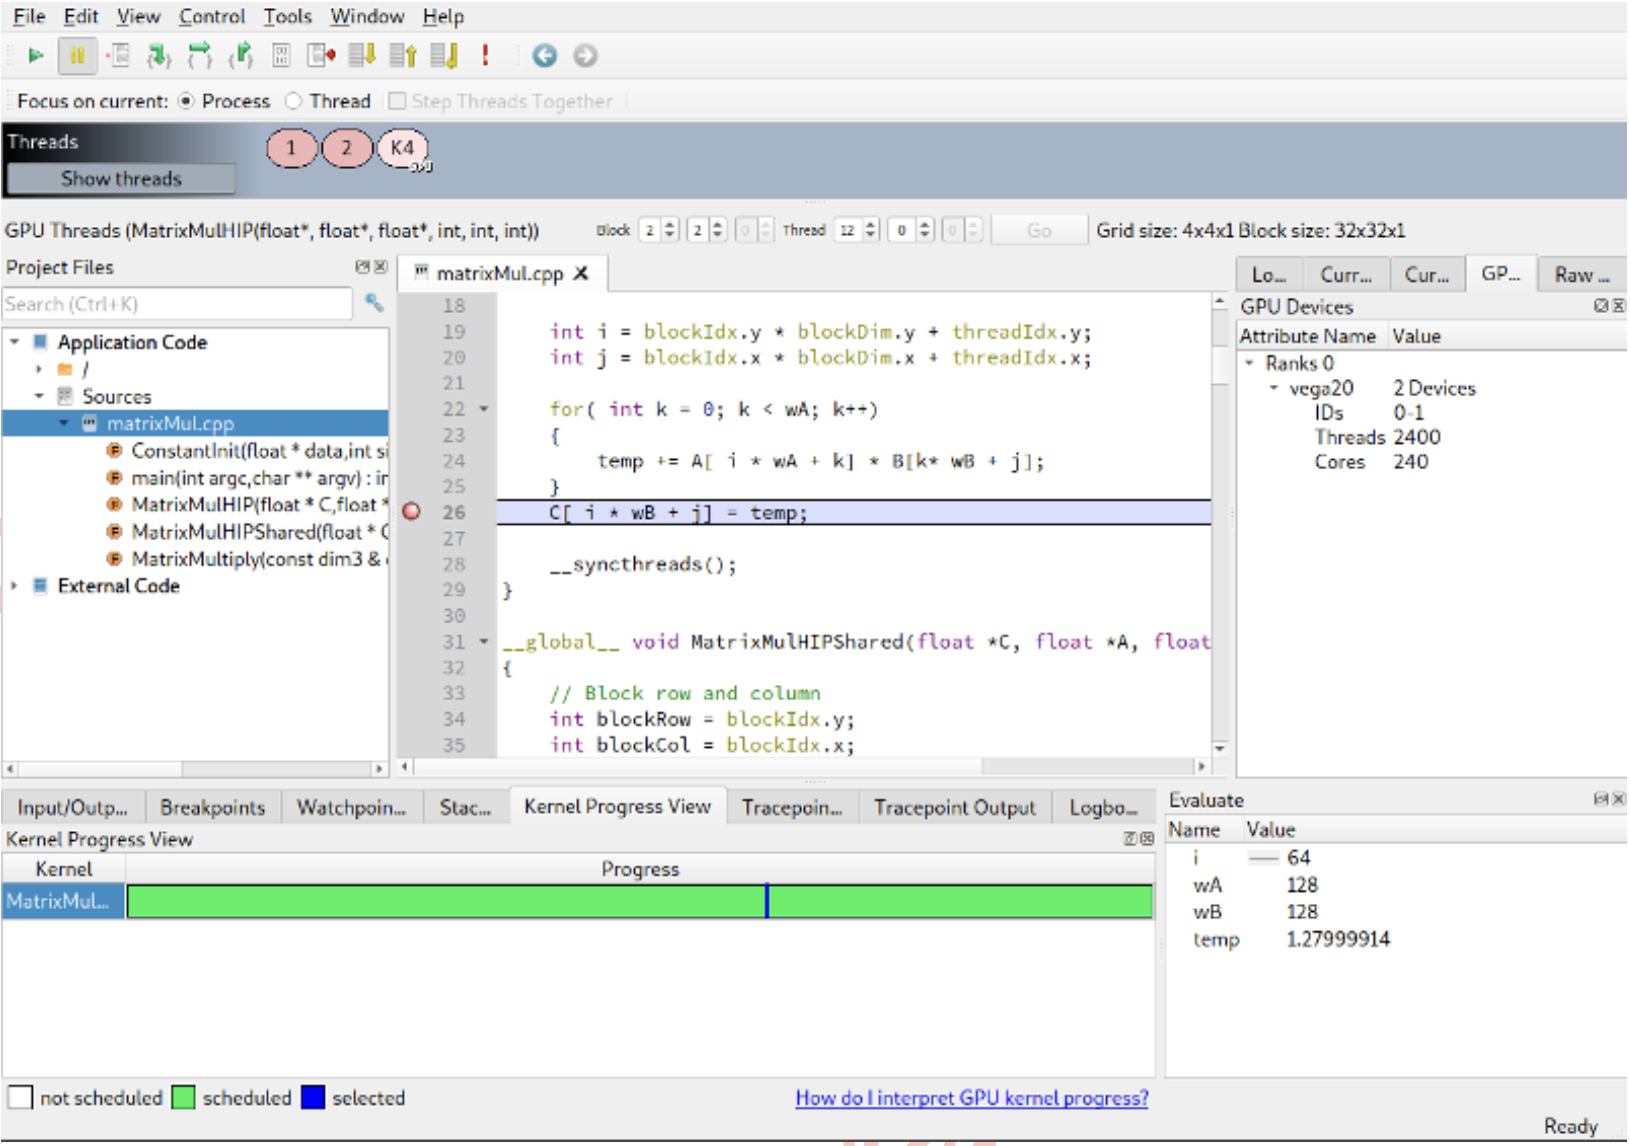
\includegraphics[width=0.9\linewidth]{FileAusiliari/Screenshots/Figure13-30.png}
    \caption{使用 Linaro DDT debug HIP 應用程式。}
    \label{fig:PAPI30}
\end{figure}

確保在點擊 Run/Submit 之前,在運行對話框中選擇 ROCm。要控制 GPU 執行緒,可以使用標準的播放、暫停和斷點控制功能。這些功能同樣適用於控制 GPU kernel的執行。然而,由於 GPU 的執行模型與 CPU 不同,因此存在一些行為上的差異,如下所述。

GPU 斷點的設置方式與其他斷點相同。在 Source Code viewer 中右鍵點擊希望設置斷點的位置,然後選擇添加斷點。斷點會影響所有 GPU 執行緒,當執行緒到達該斷點時,程式會停止。

GPU 的執行模型與host CPU 的執行模型明顯不同。在執行單步操作(如 step in、step over 或 step out)時,有一些關鍵的不同點需要注意。GPU 上最小的執行單元是 wavefront,在當前的 AMD GPU 上,每個 wavefront 包含 64 個執行緒。wavefront 中的所有執行緒以鎖步方式執行,這意味著無法單獨對每個執行緒進行單步操作。

點擊 Play/Continue 可運行所有 GPU 執行緒。可以使用 條件斷點在特定的塊、wavefront 或執行緒處暫停執行。然而,在這種情況下,該 wavefront 中的所有執行緒都會停止。點擊 Pause 可暫停正在運行的kernel。

\begin{figure}
    \centering
    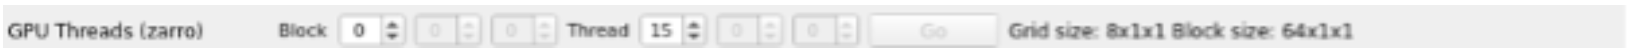
\includegraphics[width=0.9\linewidth]{FileAusiliari/Screenshots/Figure13-31.png}
    \caption{GPU thread選擇器。}
    \label{fig:PAPI31}
\end{figure}

在處理 GPU 時,大多數用戶介面與常規的 MPI 或多執行緒除錯保持不變。然而,為了幫助除錯 GPU 程式,添加了一些增強功能和附加功能。

Thread Selector 允許您選擇當前的 GPU 執行緒。當前選擇的執行緒將用於變數評估視窗,以及各種 GPU 單步操作。

在 圖 13.31 中,第一個條目指定了區塊索引。隨後的條目指定了該區塊內的 3D 執行緒索引。更改當前執行緒會更新局部變數、評估結果、當前顯示的行,還會更新顯示的源碼,為您提供 GPU kernel狀態的視角。Thread Selector 還會顯示程式中網格和區塊的維度。只有在被加載到 GPU 的區塊集合中,才能檢視/控制執行緒。如果您嘗試選擇當前未加載的執行緒,將顯示一條消息。當有活動的 GPU kernel 時,Thread Selector 才會顯示。

\begin{figure}
    \centering
    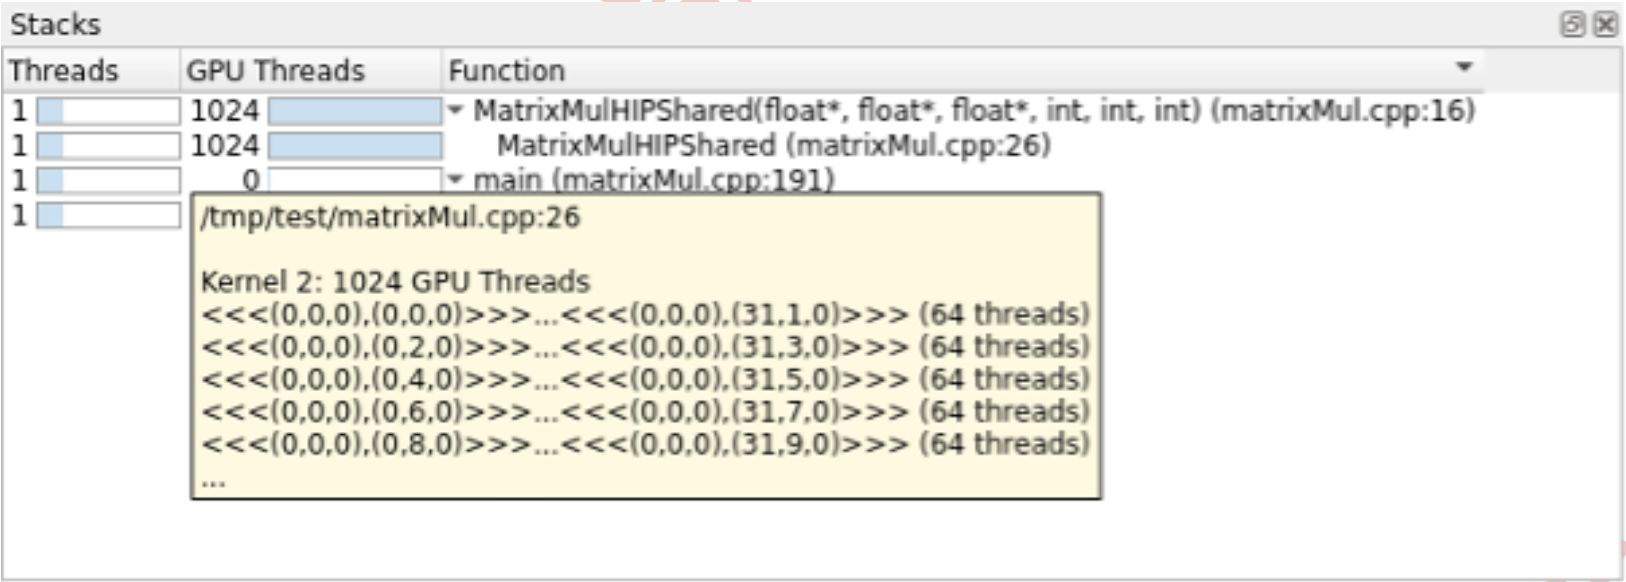
\includegraphics[width=0.9\linewidth]{FileAusiliari/Screenshots/Figure13-32.png}
    \caption{平行堆疊視圖中的 GPU thread。}
    \label{fig:PAPI32}
\end{figure}

如 圖 13.32 所示,Parallel Stack View 顯示了 GPU 執行緒的位置和數量。點擊 Parallel Stack View 中的一個項目即可選擇該框架中的 GPU 執行緒,隨之更新變數顯示組件,並將 Source Code viewer 移動到相應的位置。

要查看哪些具體的 GPU 執行緒範圍位於特定位置,以及每個範圍的大小,可將滑鼠懸停在 Parallel Stack View 中的一個項目上。


\subsubsection{Kernel Progress View}

\begin{figure}
    \centering
    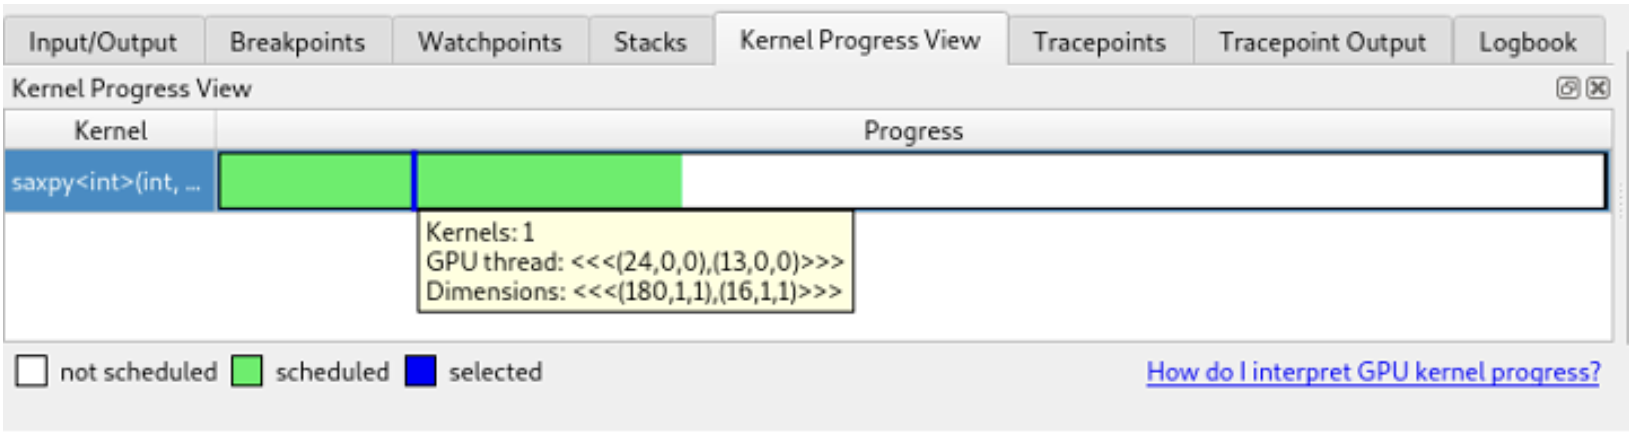
\includegraphics[width=0.9\linewidth]{FileAusiliari/Screenshots/Figure13-33.png}
    \caption{Kernel Process View中的 GPU thread。}
    \label{fig:PAPI33}
\end{figure}

如 圖 13.33 所示,當一個kernel正在執行時,Kernel Progress View 標籤會預設顯示在用戶介面的底部。此視圖提供必要的細節,以幫助您在除錯過程中判斷陣列數據是新鮮的還是陳舊的(即,該陣列是否與活動執行緒相關聯)。

對於一個為陣列中每個索引計算輸出值的簡單kernel來說,很難檢查陣列中特定位置 x 的值是否已被計算,或者計算該值的執行緒是否已被調度。這與標量程式設計形成鮮明對比,後者中如果一個(向上)迴圈的計數器超過 x,那麼索引 x 的值可視為最終值。

Kernel Progress View(見 圖 13.33)標識了正在進行的kernel。該視圖提供kernel的數量,並根據不同的kernel標識符(kernel名稱)按進程進行分組。彩色進度條顯示了哪些 GPU 執行緒正在執行。進度條是對 GPU 區塊和執行緒索引系統的直線投影,說明了程式中正在運行的kernel的大小。

\begin{figure}
    \centering
    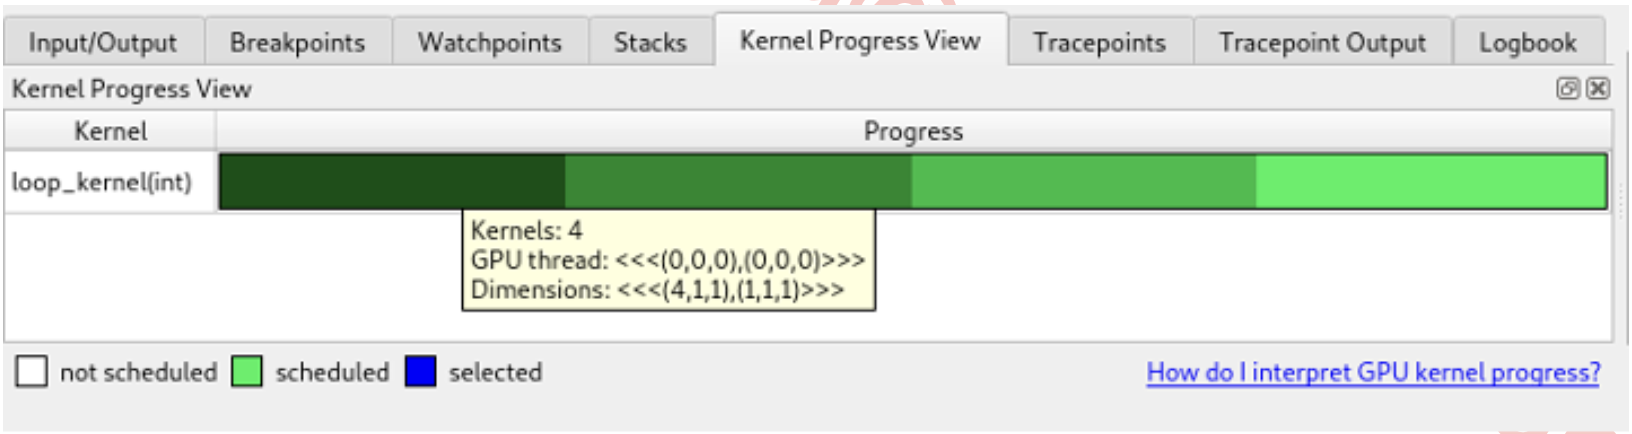
\includegraphics[width=0.9\linewidth]{FileAusiliari/Screenshots/Figure13-34.png}
    \caption{Kernel Process View中的 GPU thread。}
    \label{fig:PAPI34}
\end{figure}

點擊進度條中具有顏色高亮的部分,即可選擇一個與點擊位置最接近的執行緒。
\begin{itemize}
    \item 藍色:表示所選的 GPU 執行緒。
    \item 綠色:表示已排程運行的 GPU 執行緒。多個已排程的執行緒以不同深淺的綠色區分。
    \item 白色:表示進度條中的非活動區域。它們處於非活動狀態可能是因為已經運行過,或者未被排程運行。
    \item 擁有相同名稱的kernel會被堆疊,綠色的深淺會加深(見 圖 13.34)。
    \item 擁有不同名稱的kernel顯示在單獨的行中。
\end{itemize}


\subsubsection{原始碼檢視器}

Source Code viewer 幫助您通過高亮顯示當前堆疊追蹤中的行來可視化程式碼中的程式流程。在除錯 GPU kernel時,它會對具有可用 GPU 執行緒的行進行顏色高亮,並以類似於常規 CPU 執行緒和進程的方式顯示 GPU 執行緒。

要查看高亮行上 GPU 執行緒的摘要,可將滑鼠懸停在 Source Code viewer 中的該行上。


\subsubsection{GPU裝置資訊}

\begin{figure}
    \centering
    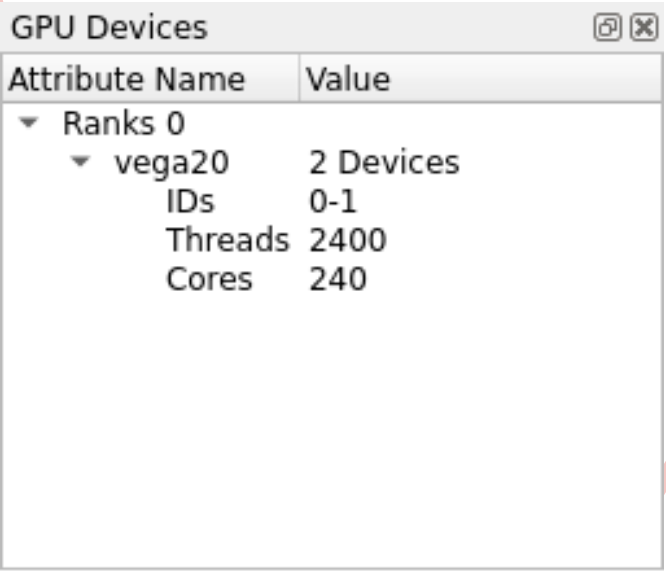
\includegraphics[width=0.4\linewidth]{FileAusiliari/Screenshots/Figure13-35.png}
    \caption{GPU 裝置 Tab}
    \label{fig:PAPI35}
\end{figure}

GPU 程式設計的一個挑戰是發現device參數,例如device類型以及device是否存在。GPU Devices 標籤(見 圖 13.35)列出了程式中存在並被使用的 GPU,並為多進程系統提供了可擴展的分組資訊(基於相似特性,如 GPU 型號進行分組)。

\subsection{使用 Linaro MAP 進行 GPU 分析}

\begin{figure}
    \centering
    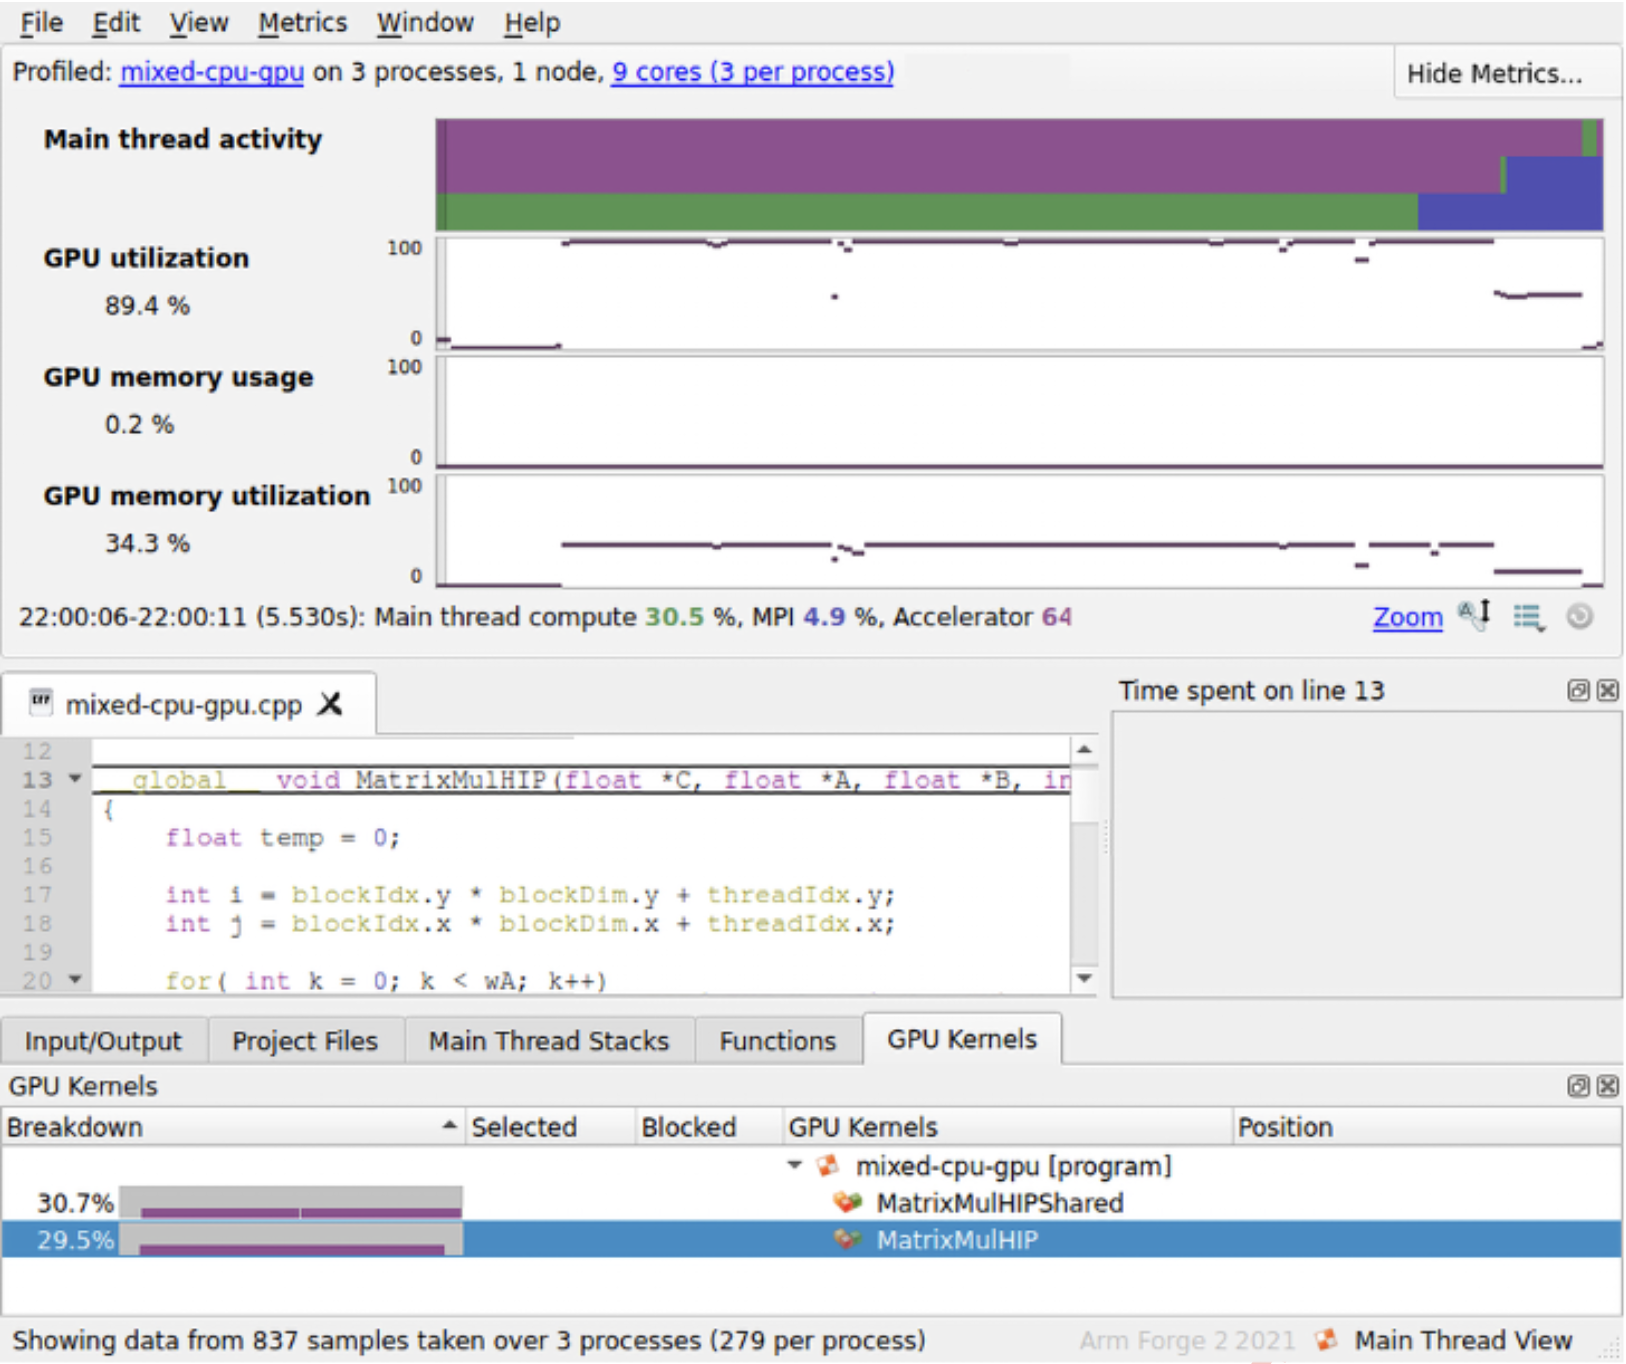
\includegraphics[width=0.9\linewidth]{FileAusiliari/Screenshots/Figure13-36.png}
    \caption{使用 Linaro MAP 對 HIP 應用程式進行分析。}
    \label{fig:PAPI36}
\end{figure}

在處理 AMD ROCm 程式時,可以使用 Linaro MAP 的 GPU 剖析功能。當檢測到 ROCm 函式庫時,AMD GPU 剖析會預設啟用。在使用 AMD ROCm CPU 的程式中,等待 GPU kernel完成的時間會以紫色顯示。

在 圖 13.36 中,展示了一個混合了 MPI 和 HIP 的應用程式範例,其中兩個進程各自執行了一個 HIP kernel,另一個進程則以串行方式執行。

要在 Linaro MAP 中查看源碼,請使用以下方式啟用除錯標誌編譯程式。請勿使用純除錯構建。在使用 Linaro MAP 進行剖析時,請始終保持啟用最佳化標誌:

\begin{lstlisting}
$ hipcc -g -O3 -o program_name source_file.cpp
\end{lstlisting}

開啟Linaro MAP:
\begin{lstlisting}
$ map <program_name> [arguments]
\end{lstlisting}

如果您使用 Linaro Forge Professional,AMD ROCm GPU 加速器指標會預設啟用。這些指標可以通過 AMD ROCm 的預設選單選項進行選擇。圖 13.37 中展示了這些指標的範例。

指標包括:

\begin{itemize}
    \item GPU 利用率:GPU 使用的百分比,包括一個或多個kernel在 GPU 卡上執行。如果計算節點上存在多張卡,該值為該節點上所有卡的平均值。
    \item GPU 記憶體使用率:GPU 上已分配的記憶體,作為 GPU 可用記憶體總量的百分比。
    \item GPU 記憶體利用率:GPU 記憶體使用的時間百分比。如果計算節點上存在多張卡,該值為該節點上所有卡的平均值。
\end{itemize}

\begin{figure}
    \centering
    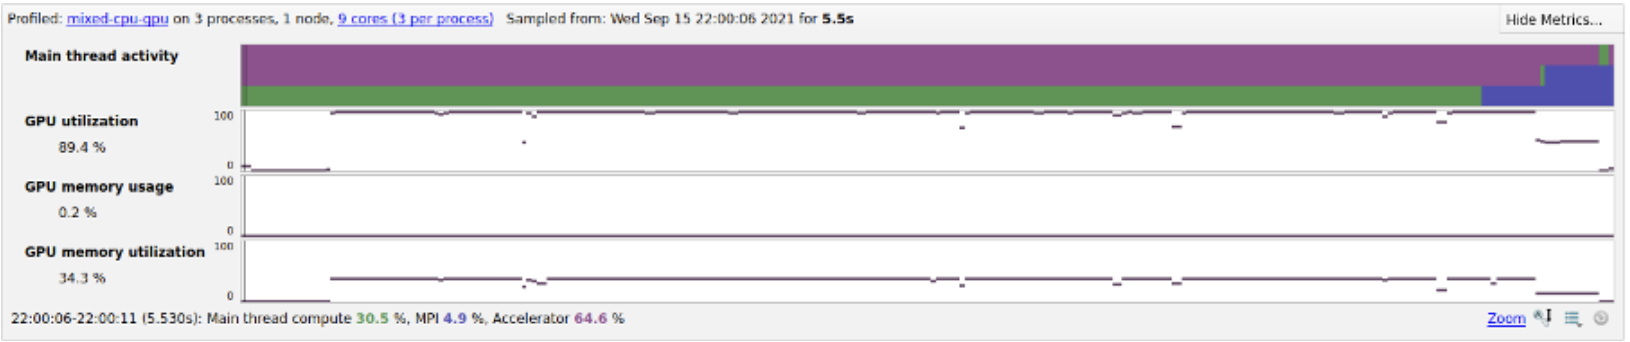
\includegraphics[width=0.9\linewidth]{FileAusiliari/Screenshots/Figure13-37.png}
    \caption{Linaro MAP 中的 ROCm GPU 指標視圖。}
    \label{fig:PAPI37}
\end{figure}

在剖析 AMD GPU 程式時,可追蹤的 GPU kernel將顯示在 GPU Kernels 標籤中,如 圖 13.38 所示。

\begin{figure}
    \centering
    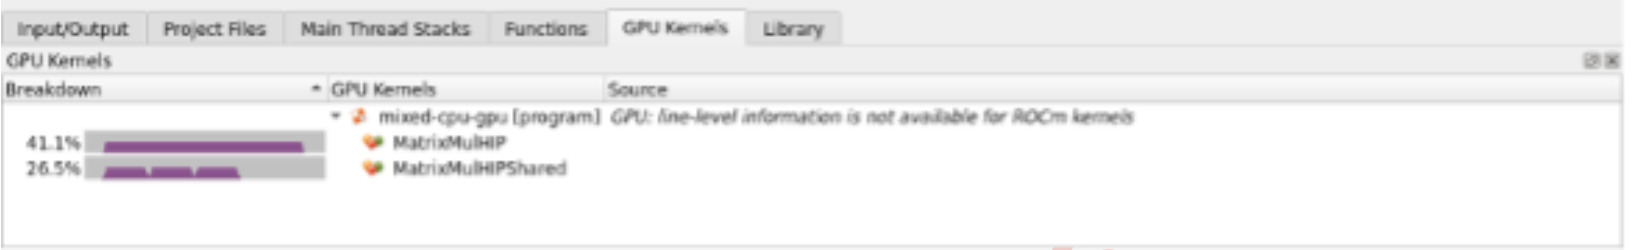
\includegraphics[width=0.9\linewidth]{FileAusiliari/Screenshots/Figure13-38.png}
    \caption{Linaro MAP中的GPU Kernels Tab。}
    \label{fig:PAPI38}
\end{figure}

此視圖列出了程式中檢測到的 GPU kernel,並附有圖表顯示它們處於活動狀態的時間。如果在特定的剖析樣本中同一進程內檢測到多個kernel,這些kernel在圖表中被賦予相等的權重。選擇單個 GPU kernel時,如果有可用的除錯資訊,Source Code viewer 會跳轉到該kernel的源碼位置。

\subsection{GPU效能報告}

要生成 Linaro Performance Reports 報告,請執行以下命令:
\begin{lstlisting}
$ perf-report <program_name> [arguments]
\end{lstlisting}

程式會正常運行。程式完成後,性能報告會以 HTML 和 文本格式保存到當前工作目錄中,文件名基於應用程式的可執行檔生成。

對於 AMD ROCm 應用程式,加速器指標和建議會顯示在報告中,如 圖 13.39 所示。

\begin{figure}
    \centering
    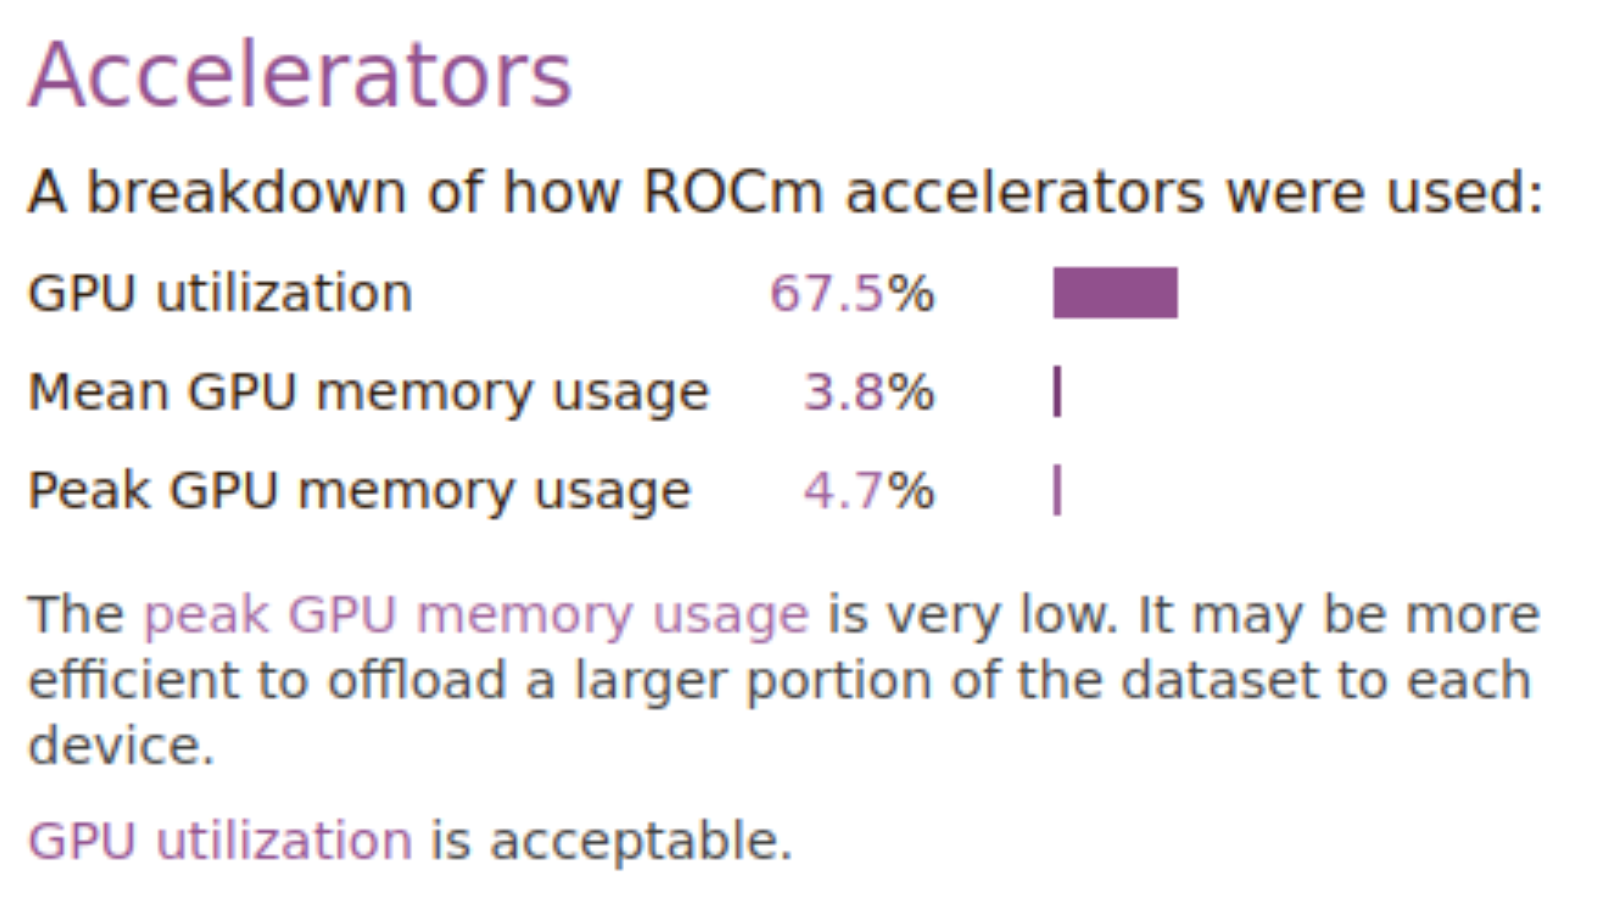
\includegraphics[width=0.9\linewidth]{FileAusiliari/Screenshots/Figure13-39.png}
    \caption{加速器指標報告。}
    \label{fig:PAPI39}
\end{figure}

報告中的指標包括:
\begin{itemize}
    \item GPU 利用率:GPU 上一個或多個kernel執行的時間百分比,取所有可用 GPU 的平均值。
    \item 平均 GPU 記憶體使用量:GPU 卡上使用的記憶體平均值。
    \item 峰值 GPU 記憶體使用量:GPU 卡上使用的記憶體最大值。
\end{itemize}

更多有關 Linaro Forge 的下載與資訊,請訪問:
https://www.linaroforge.com/


\section{E4S - 超大規模科學軟體堆疊}

\begin{figure}
    \centering
    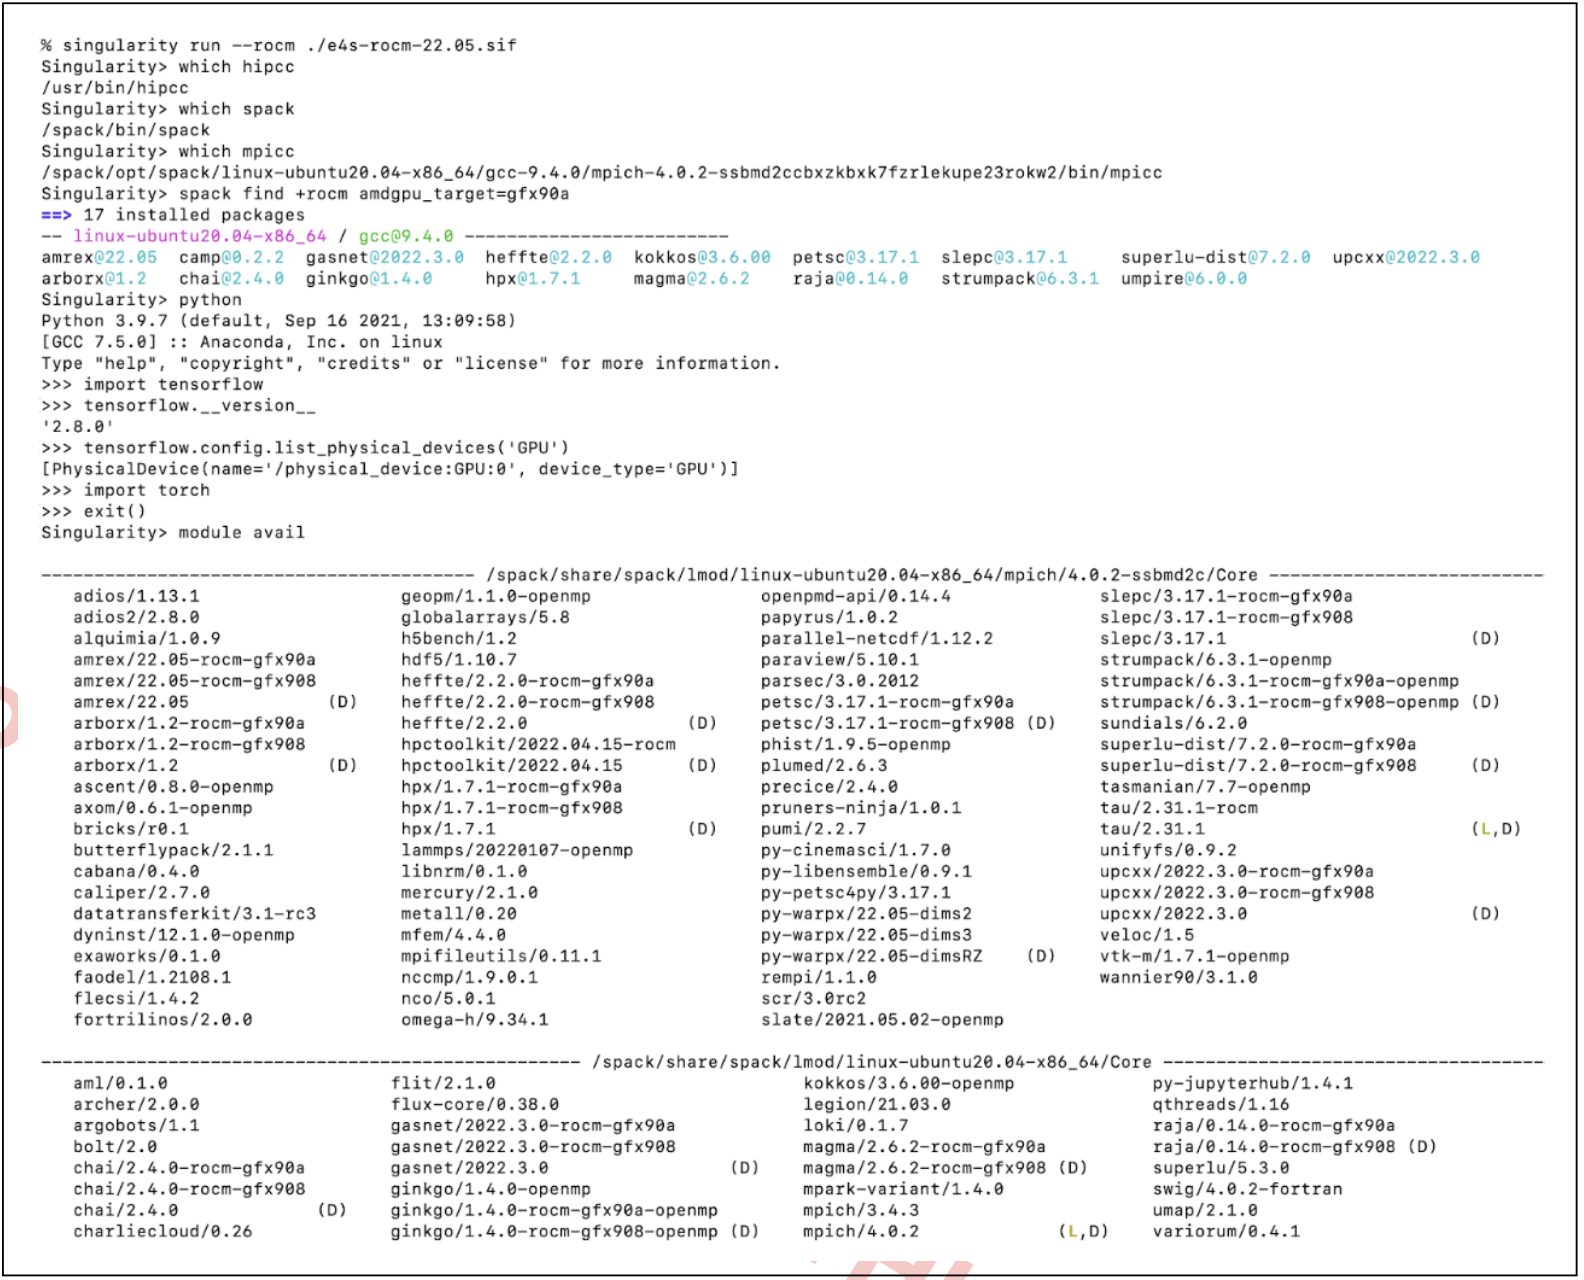
\includegraphics[width=0.9\linewidth]{FileAusiliari/Screenshots/Figure13-40.png}
    \caption{E4S Singularity 映像 顯示了支持 MI210 AMD GPU 的已安裝 HPC 和 AI/ML 工具列表。}
    \label{fig:PAPI40}
\end{figure}

E4S [52] 是基於 Spack 套件管理器 [25] 的精選軟體產品集合。它包括可下載和自定義的完整功能和基礎容器映像。這些容器映像支援 Docker 和 Singularity [68] 容器運行時。

除了包含超過 100 個 HPC 工具和數值庫外,E4S 映像還包括完整的 ROCm,內含編譯器(hipcc)和基於 Python 的人工智慧(AI)與機器學習(ML)工具,如 PyTorch 和 TensorFlow,針對 AMD GPU。E4S 基礎映像僅包含 ROCm 和 MPI。用戶可以使用 Spack 構建自定義容器映像。

E4S 還包含一個獨特的工具(即 e4s-cl [52]),常用於啟動 MPI 應用程式。MPI 庫位於容器映像中,可以替換為系統上的對應庫。在運行時替換 MPI 未修改的二進位檔,使程式設計師能利用高性能網路(如 InfiniBand),在數據中心節點間進行快速的節點間通信。

E4S 是一個不斷增長的工具和庫套件,旨在降低 HPC 和 AI/ML 程式設計師的入門門檻。通過使用現成的 E4S 容器,E4S 使新用戶能輕鬆地在大規模運行中利用 ROCm 的優勢。


最新的 E4S 版本 22.05 提供了完整功能和基礎映像,支援 ROCm 版本 5.1.1 和 gfx90a(MI210/MI250X+),以及 gfx908(MI100)架構。圖 13.40 展示了一個會話,其中 HPC 和 AI/ML 套件(例如 TensorFlow 版本 2.8.0 和 PyTorch 版本 1.11.0)已配置為使用 AMD GPU。

工具可通過 Spack 套件管理器安裝到此 Singularity 映像中,Spack 提供模組和 Spack CLI。容器映像中包括 MPI、數值庫和工具、編譯器、建構工具(如 cmake 和 autotools)以及圖形化工具。最新版本的性能評估工具(如 PAPI [70]、TAU [64] 和 HPCToolkit [83])通過 rocProfiler 和 rocTracer 插桿介面為 AMD GPU 提供支援。這些工具在容器環境中運行非常有效。

E4S 完整功能映像 包含超過 100 個使用 Spack、ROCm、MPI 和其他建構工具構建的套件。而 E4S 基礎映像 僅包含 Spack、ROCm、MPI 和建構工具,但不包含其他 AI/ML 或 HPC 套件。不過,程式設計師可以靈活地從此基礎映像構建自定義且緊湊的容器映像。這些衍生映像可以使用 Docker、Singularity 或 Shifter 容器運行時啟動。

E4S 的目標是讓所有 HPC 和 AI/ML 程式設計師能夠構建自己的應用程式,並部署支持 GPU 的常用工具和庫的 E4S 容器。這些映像可以部署在工作站或數據中心中的大規模 HPC 系統上,為使用最新 AMD GPU 的應用程式提供一致的開發和部署環境。

